% TODO:
% prepisi proceduro Multiply v javo
\documentclass[a4paper,10pt]{article}
\usepackage[slovene]{babel}
\usepackage{graphicx}
\usepackage{hyperref}
\usepackage{listings}
\usepackage{epsfig}
\lstset{numbers=left, frame=single}
\usepackage{amsmath}
\usepackage{amsfonts}
\usepackage{amssymb}
\usepackage{float}
\usepackage{floatflt}

\begin{document}
\title{Zapiski s predavanj predmeta Algoritmi in podatkovne strukture 2}
\author{Alenka Caserman}
\maketitle

\tableofcontents

\part{Pozor}
Zaradi obse\v znosti teh zapiskov je mogo\v ce, da se \v se kje skriva kak\v sna napaka. \v Ce jo odkrijete vas prosim, da jo sporo\v cite na e-mail naslov alenka [pika] caserman [afna] gmail [pika] com.\\
Vabim vas tudi da prispevate kak\v sno dodatno gradivo kot so npr. primeri algoritmov, pripomo\v cki za vizualizacijo, podrobnej\v se razlage itd.\\
V leto\v snjem letu imam v na\v crtu pripraviti tudi podobno skripto za pomo\v c pri vajah. \v Ce vas zanima sodelovanje me kontaktirajte preko e-maila.
Hvala!\\

\part{Uvod}

\section{Algoritmi}
Algoritem je nekak\v sen program, ki te\v ce na nekem ra\v cunalniku. Ra\v cunalnik na katerem algoritem te\v ce pa je lahko bodisi resni\v cen bodisi nami\v sljen (model ra\v cunanja).

\paragraph{Algoritem:}
\begin{itemize}
\item dobi neke podatke $\Rightarrow$ VHOD
\item vrne neke podatke $\Rightarrow$ IZHOD
\end{itemize}

\begin{figure}[h]
	\centering
	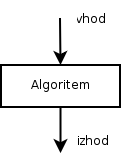
\includegraphics[width=2.45cm,height=3.25cm]{Slike/Algoritem}
% Algoritem.: 50.8dpi, width=2.45cm, height=3.25cm, bb=0 0 49 65
	\caption{Diagram preprostega algoritma}
\end{figure}

\paragraph{Va\v zno:} za vsak vhod je izhod natan\v cno definiran oz. dolo\v cen: $\forall$ vhod: izhod = algoritem(vhod). Kadar to ne velja ve\v c, to ni ve\v c algoritem ampak procedura (recept za izra\ cun).

\subsection{Modeli ra\v cunanja (nami\v sljeni ra\v cunalnik)}
Poznamo jih veliko, npr. T\"uringov stroj, avtomati, RAM, $\lambda$ -funkcije, rekurzivne funkcije, programi v raznih programskih jezikih, diagram poteka,...

\subsubsection{RAM (Random Access Machine)}
\begin{itemize}
\item stroj z enakopravnim dostopom do pomnilnika
\item je dovolj podoben obstoje\v cim, resni\v cnim ra\v cunalnikom
\item procesor:
\begin{itemize}
	\item lahko izvaja obi\v cajne operacije (aritmeti\v cne operacije, operacije nad biti, preusmerjanje - skoki,...)
	\item zaporedno izvaja ukaz za ukazom
	\item vsaka operacija traja enoto \v casa
	\end{itemize}
\item pomnilnik:
	\begin{itemize}
	\item celice (besede) so enako dosegljive za procesor
	\item vsebuje podatke (program) poljubne velikosti (pomnilni\v ska beseda nima omejene dol\v zine)
	\end{itemize}
\end{itemize}

\paragraph{Zanemarimo:}
\begin{itemize}
\item druge komponente ra\v cunalnika, npr. V/I enote
\item druge podrobnosti, npr. zaokro\v zitvene napake, ker pomnilni\v ska beseda nima omejene dol\v zine
\end{itemize}

\paragraph{PRAM:} vzporedni algoritmi, ve\v c procesorjev

\paragraph{Prednosti RAM-a:}
\begin{itemize}
\item dokaj stvarna (realna) ocena porabljenega \v casa (\v stevilo izvedenih ukazov, vsak je dolg enoto \v casa)
\item realna ocena poraljenega prostora (\v stevilo porabljenih celic v pomnilniku)
\end{itemize}

\paragraph{Pomanjkljivosti RAM-a:}
\begin{itemize}
\item algoritmi, ki jih pisemo za ta model so dokaj nepregledni (bistvo algoritma se zgubi)
\end{itemize}

\paragraph{Posledica:}
RAM si predstavljamo kot \textbf{ciljni stroj}, algoritme pa bomo opisali v nekem \textbf{vi\v sjem programskem jeziku}.

\paragraph{Vi\v sji jeziki} za zapis algoritmov so namenjeni:
\begin{enumerate}
\item \textbf{\v cloveskemu bralcu}: prirejeni jezki algolskega tipa, poenostavitve Algola, Pascala, Modula,...
\item \textbf{izvajanju na stvarnem ra\v cunalniku} (Java, C, Oberon-2)
\end{enumerate}

\paragraph{Primer algoritma za dvoji\v sko iskanje:}
\begin{flushleft}
VHOD:
\end{flushleft}
\begin{itemize}
\item a - tabela nekih elementov, urejena z relacijo manj\v si
\item n - \v st. elementov v tabeli
\item x - element za katerega nas zanima, \v ce je v tabeli, \v e ga ni pa kam bi sodil
\end{itemize}

\begin{flushleft}
IZHOD:
\end{flushleft}

\begin{itemize}
\item indeks iskanega elementa v a (\v ce $x \in a$), sicer pa negativni indeks, kamor bi element sodil (\v ce $x \notin a$)
\end{itemize}

\paragraph{Bistvo algoritma:}
\v Ce x sodi v del med indeksoma l in r, potem poglej, \v cr je na \textbf{sredini} med l in r. \v Ce ni, nadaljuj iskanje v tistem delu kamor sodi po velikosti, tj. \textbf{levo} ali \textbf{desno} od srednjega.
	\begin{center}
	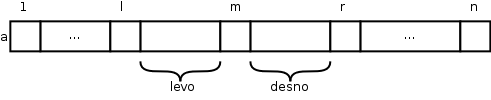
\includegraphics[width=9.65cm,height=1.95cm]{Slike/BinarniSortTabela.png}
% BinarniSortTabela.png: 50.8dpi, width=9.65cm, height=1.95cm, bb=0 0 193 39
	\end{center}

\paragraph{Koda:}
\begin{flushleft}
% TODO: prepisi kodo za binarno iskanje v Javo ali C
\begin{lstlisting}[language=Pascal,caption={Koda za metodo binarnega iskanja}]
PROCEDURE BinSearch(VAR a: ARRAY OF INTEGER;
		      x,n: INTEGER) : INTEGER
VAR l,m,r : INTEGER;
BEGIN l:=1, r:=n;...iscemo v celotni tabeli a
	WHILE l<=r DO...dokler obstaja nepregledan del tabele a
		m:=(l+r) DIV 2;
		IF a[m]>x THEN r:=m-1;
		ELSE l:=m+1;
	END
	IF (r > 0) && (a[r] =x) THEN RETURN r;
	ELSE RETURN -l;
END BinSearch;
\end{lstlisting}
\end{flushleft}

\paragraph{Sled programa}
Je tabela parov izbrane vrstice programa v delovanju in vrednosti izbranih spremenljivk, ki priprada programu (algoritmu) in konkretnemu vhodu. Uporabljamo jo za opazovanje delovanja programa.
\begin{table}[h]
\centering
\begin{tabular}{|c|c|}\hline
\v st. izbrane vrstice programa v delovanju & vrednosti izbranih spremenljivk \\\hline
 & \\
 &
\end{tabular} 
\caption{Tabela sledi}
\end{table}


Npr. za BinSearch in za $a=(9, 13, 27, 32, 41, 48), x=18$:

\begin{table}[h]
\centering
\begin{tabular}{c|ccc}
vrstica & l & m & r\\\hline
4 & 1 & - & 6\\
6 & 1 & 3 & 6\\
7 & 1 & 3 & 2\\
6 & 1 & 1 & 2\\
8 & 2 & 1 & 2\\
6 & 2 & 2 & 2\\
8 & 3 & 2 & 2\\\hline
6 & 3 & 2 & 2\\
\end{tabular}
\caption{Tabela sledi za BinSearch}
\end{table}

\paragraph{Drevo sledi} je sestavljeno iz ve\v c sledi(vsaka sled za drug vhod).

\begin{figure}[hbt]
	\centering
	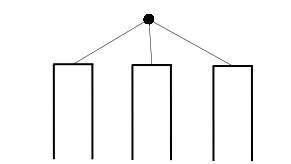
\includegraphics[width=5.75cm,height=3.25cm]{Slike/DrevoSledi.png}
% DrevoSledi.png: 50.8dpi, width=5.75cm, height=3.25cm, bb=0 0 115 65
\caption{Drevo sledi}
\end{figure}

\section{Preverjanje pravilnosti  algoritmo/programov}
V praksi je velikokrat pomembno vedeti, \v ce je algoritem pravilen. \\
\textbf{Kako dokazati oz. preveriti pravilnost algoritma?} \\
Dva pristopa:
\begin{enumerate}
\item s poskusi
\item z logi\v cno analizo
\end{enumerate}

\subsection{Preverjanje pravilnosti s poskusi}
\paragraph{Zamisel}
Na izbranih (nekaterih) vhodih preveri, \v ce so sledi OK (pravilne, taksne kot morajo biti).

\paragraph{Velja}
\v Ce kaka sled ni OK $\Rightarrow$ algoritem ni pravilen oz. \v ce so vse mozne sledi OK $\Rightarrow$ algoritem je pravilen. Vseh mo\v znih sledi pa je lahko ogromno:
\begin{itemize}
\item kon\v cno
\item neskon\v cno
\begin{itemize}
\item \v stevno mnogo
\item kontinuum
\end{itemize}
\end{itemize}

Najve\v ckrat pa je vseh mo\v znih sledi preve\v c.\\

\paragraph{Primer:} mno\v zenje s se\v stevanjem $\Rightarrow$ kako pomno\v ziti dve \v stevili med seboj brez operacije mno\v zenja

\paragraph{Zamisel:} $x \ast y = y + y + ... + y (x>0)$

\paragraph{Algoritem}
\begin{flushleft}
% TODO: prepisi v Javo ali C
\begin{lstlisting}[language=Pascal,caption={Koda za metodo mno\v zenja s se\v stevanjem}]
PROCEDURE Muliply(x,y : INTEGER) : INTEGER
VAR u,z : INTEGER;
BEGIN z:=0, u:=x;
	REPEAT z:=z+y; u:=u-1;
	UNTIL u:=0;
	RETURN z;
END Multiply;
\end{lstlisting}
\end{flushleft}
\v Stevilo vhodov je $2^{16} \cdot 2^{16} = 2^{32}$ (ker je INTEGER v Oberonu 16-biten). Iz tega sledi, da bi bilo treba preveriti $2^{32}$ sledi, kar je v praksi nesmiselno. Preverjanje s poskusi v praksi ni zelo uporabno, razen za iskanje napak oz. dokazovanje nepravilnosti. Potreben je druga\v cen pristop.

\subsection{Preverjanje pravilnosti programov z logi\v cno analizo}

\paragraph{Zamisel}
Z logi\v cnim sklepanjem ugotoviti ali iz lastnosti algoritma in lastnosti vhoda sledi tudi \v zeljena lastnost algoritma.\\
\textbf{Kako izraziti lastnost?} \\
S predikatnim ra\v cunom 1. reda:
\begin{itemize}
\item stavki - lastnosti
\item pravila sklepanja
\end{itemize}

\subsubsection{Logi\v cna analiza na diagramih poteka}

Diagram poteka je:
\begin{itemize}
\item usmerjen graf
\item en vhod, en ali ve\v c izhodov
\item 3 vrste vozli\v s\v c
\end{itemize}

\begin{figure}[h]
	\centering
	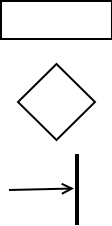
\includegraphics[width=2.2cm,height=4.45cm]{Slike/DiagramPotekaSimboli.png}
% DiagramPotekaSimboli.png: 50.8dpi, width=2.20cm, height=4.45cm, bb=0 0 44 89
	\caption{Simboli za diagram poteka}
\end{figure}

\paragraph{Primer: Mno\v zenje s se\v stevanjem}
	\begin{center}
	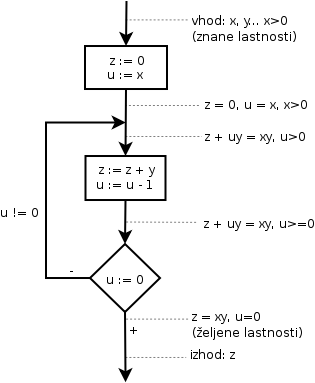
\includegraphics[width=6.2cm,height=7.55cm]{Slike/MnozenjeSSestevanjem.png}
% MnozenjeSSestevanjem.png: 50.8dpi, width=6.20cm, height=7.55cm, bb=0 0 124 151
	\end{center}

\paragraph{Primer: Deljenje s pomo\v cjo od\v stevanja}
	\begin{center}
	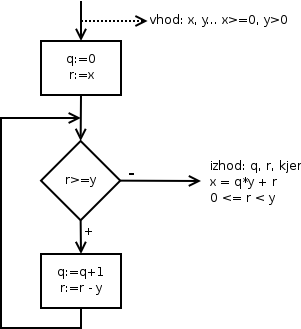
\includegraphics[width=5.95cm,height=6.5cm]{Slike/DeljenjeZOdstevanjem.png}
% DeljenjeZOdstevanjem.png: 50.8dpi, width=5.95cm, height=6.50cm, bb=0 0 119 130
	\end{center}
\textbf{Kako v na\v celu poteka dokazovanje pravilnosti?} \\
Izhajamo iz:
\begin{itemize}
\item znanih lastnosti vhoda
\item \v zeljenih lastnosti izhoda
\end{itemize}
Vsakemu vozli\v s\v cu pripi\v semo mno\v zico trditev:
\begin{itemize}
\item po eno trditev na vsako vhodno povezavo
\item po eno trditev na vsako izhodno povezavo
\end{itemize}
\textbf{Kako?}\\
Tako, da velja sklep:
\begin{quote}
\v Ce pred izvedbo S velja A, potem po izvedbi S velja C.
\end{quote}
To je odvisno od tipa in pomena S.

\paragraph{Cilj}
Dani algoritem
	\begin{center}
	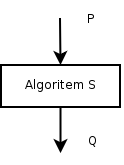
\includegraphics[width=2.45cm,height=3.25cm]{Slike/AlgoritemS}
	\end{center}
opisati kot zaporedje korakov
	\begin{center}
	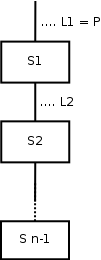
\includegraphics[width=2cm,height=5.1cm]{Slike/ZaporedjeKorakov.png}
% ZaporedjeKorakov.png: 50.8dpi, width=2.00cm, height=5.10cm, bb=0 0 40 102
	\end{center}
tako da velja: $\forall : i=1, 2,... u-1$, \v ce pred $S_i$ velja $L_i$, po $S_i$ velja $L_{i+1}$.

\subsubsection{Aksiomi}
\begin{itemize}
\item za \textbf{stekali\v sce}:
	\begin{quote}
	\v Ce velja nekaj pred stekali\v scem, naj velja tudi po njem.
	\end{quote}
	\begin{center}
	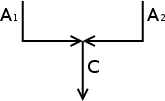
\includegraphics[width=3.25cm,height=2cm]{Slike/Stekalisce.png}
% Stekalisce.png: 50.8dpi, width=3.25cm, height=2.00cm, bb=0 0 65 40
	\end{center}
	Kjer za C velja: $A_1\Rightarrow C \wedge A_2 \Rightarrow C$ (npr. $C = A_1 \vee A_2$).
\item \textbf{pogojni stavek}
	\begin{center}
	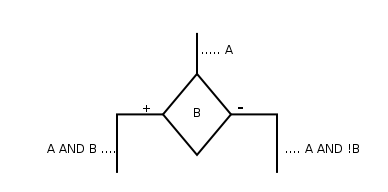
\includegraphics[width=7.65cm,height=3.8cm]{Slike/PogojniStavek.png}
% PogojniStavek.png: 50.8dpi, width=7.65cm, height=3.80cm, bb=0 0 153 76
	\end{center}

\item \textbf{prirejanje}: po prirejanju $z=f(x)$ dobimo konsekvens tako, da v antecedensu vse proste pogoje
\end{itemize}

\paragraph{Opozorilo:}
Vsaki\v c ko prispevamo v $\bigotimes$, tam velja $z + uy = xy, u>0$. To trditev imenujemo \textbf{zan\v cna invarianta}. Zanjo velja:
\begin{itemize}
\item je na za\v cetku zanke
\item je veljavna vsakokrat ob izvedbi zanke
\end{itemize}

	\begin{center}
	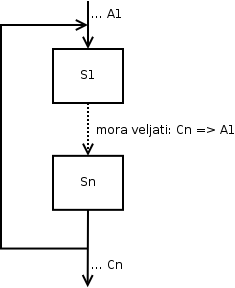
\includegraphics[width=4.65cm,height=5.65cm]{Slike/ZancnaInvarianta.png}
% ZancnaInvarianta.png: 50.8dpi, width=4.65cm, height=5.65cm, bb=0 0 93 113
	\end{center}

\subsubsection{Pravila sklepanja za ve\v cje poddiagrame}
\begin{itemize}
\item zanka WHILE, \v ce vemo da velja:
	\begin{center}
	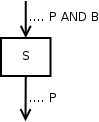
\includegraphics[width=1.95cm,height=2.4cm]{Slike/ZankaWHILE1.png}
% ZankaWHILE1.png: 50.8dpi, width=1.95cm, height=2.40cm, bb=0 0 39 48
	\end{center}
potem
	\begin{center}
	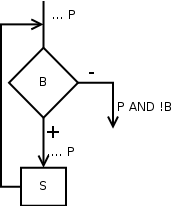
\includegraphics[width=3.35cm,height=4.05cm]{Slike/ZankaWHILE2.png}
% ZankaWHILE2.png: 50.8dpi, width=3.35cm, height=4.05cm, bb=0 0 67 81
	\end{center}
\item zanka REPEAT, \v ce vemo da velja:
	\begin{center}
	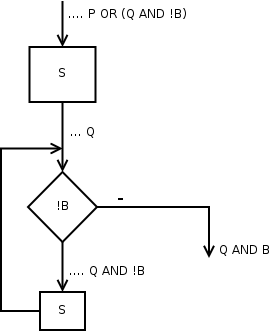
\includegraphics[width=5.3cm,height=6.5cm]{Slike/ZankaREPEAT.png}
% ZankaREPEAT.png: 50.8dpi, width=5.30cm, height=6.50cm, bb=0 0 106 130
	\end{center}
\end{itemize}

\subsubsection{Logi\v cna analiza programa v programskem jeziku}
\begin{itemize}
\item tehniko enostavno prilagodimo
\item prirejanje: $(\ast P_w^v \ast) v:=w (\ast P \ast)$
\item sestavljanje skokov: \v ce $(\ast P \ast) S_1 ()\ast Q \ast$ in $(\ast Q \ast) S_2 (\ast R \ast)$, potem $(\ast P \ast) S_1,S_2 (\ast P_v \ast)$
\item pogojni stavek: \v ce $(\ast P \wedge B \ast)\;S\;(\ast P \ast)$, potem $(\ast P \ast)$ WHILE B DO S END $(\ast P \wedge \overline{B} \ast)$
\item repeat: \v ce $(\ast P \ast)\; S \;(\ast Q \ast)$ in $(\ast Q \wedge \overline{B} \ast)\;S\;(\ast Q \ast)$, potem $(\ast P \ast)$ REPEAT S UNTIL B $(\ast Q \wedge B\ast)$
\end{itemize}

\subsection{Preverjanje ustavljanja}
Pravilnost in ustavljivst sta dva razli\v cna pojma.

\paragraph{Trditev o pravilnosti programa:}
\begin{quote}
\v Ce program pride do izstopne to\v cke, potem velja trditev Q.
\end{quote}

\paragraph{Trditev o ustavljivosti programa:}
\begin{quote}
Program po kon\v cnem \v stevilu korakov pride do izstopne to\v cke.
\end{quote}
\textbf{Kako dokazati trditev o ustavljivosti?}\\
Posku\v samo s tehniko monotono padajo\v ca funkcija.

\paragraph{Tehnika:}
\begin{enumerate}
\item izberemo neko \textbf{funkcijo f(...)}, ki je odvisna od nekaterih spremenljivk programa in ima lastnost $f(\ldots) \geq lim$ v vsaki to\v cki programa
\item diagram poteka \textbf{razdelimo na enostavne odseke} (vsak tak odsek, ki nima zanke), tako da veljata:
	\begin{itemize}
	\item vsako pot skozi diagram sestavljajo nekateri odseki (ne nujno vi in se lahko ponovijo ve\v ckrat)
	\item na vsakem odseku se vrednost funkcije f strogo zmanj\v sa (razen mogo\v ce na zadnjem, izstopnem odseku)
	\end{itemize}
\end{enumerate}
\v Ce nam uspe izvesti oba koraka lahko zaradi 1. in 2. to\v cke sklepamo, da nobena pot skozi diagram ne more imeti neskon\v cno odsekov. Iz tega sledi, da se program ustavi.
	\begin{center}
	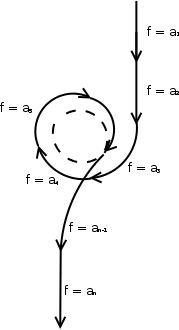
\includegraphics[width=3.5cm,height=6.5cm]{Slike/Ustavljivost.png}
% Ustavljivost.png: 50.8dpi, width=3.50cm, height=6.50cm, bb=0 0 70 130
	\end{center}
Ker $\forall \;i:\;(a_i > lim \wedge a_i>a_{i+1})$, je na vsaki poti le kon\v cno mnogo odsekov.

\paragraph{Primer: mno\v zenje s se\v stevanjem}
	\begin{center}
	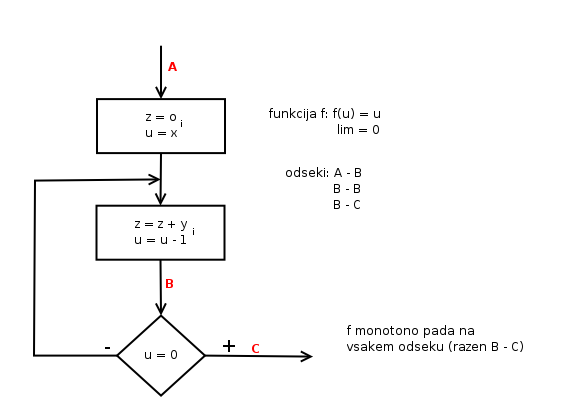
\includegraphics[width=11.2cm,height=8.25cm]{Slike/DokazovanjePravilnostiZDiagramom.png}
% DokazovanjePravilnostiZDiagramom.png: 50.8dpi, width=11.20cm, height=8.25cm, bb=0 0 224 165
	\end{center}
V praksi je tako formalno dokazovanje pravilnosti zelo te\v zko.

\section{Poraba \v casa in prostora}

\subsection{Poraba \v casa}

Naj bo T(s) \v cas za izvedbo stavka S. Osnovna lastnost, ki je predpostavljena:
$$T(S_1,S_2) = T(S_1) + T(S_2)$$
Velja za ra\v cunske modele, kjer se $S_2$ za\v cne \v sele, ko se je izvedel $S_1$ (model zaporednega ra\v cunanja), torej velja tudi za RAM. V dana\v snjih ra\v cunalnikih pa imamo ve\v c procesorjev, ki v\v casih lahko izvedejo $S_1$ in $S_2$ vzporedno. Tam na\v sa predpostavljena osnovna lastnost ne velja vedno.

\subsection{Poraba prostora}

Pomnilni prostor sestavljajo razni deli:
\begin{itemize}
\item prostor za program
\item prostor za spremenljivke
\item prostor za sklad
\item prostor za dinami\v cno zasedanje/spro\v scanje
\end{itemize}
Naj bo M(X) prostor za spremenljivko X. Osnovna lastnost:
$$M(X_1 \cup S_2) = M(X_1) + M(X_2)$$
Velja za model ra\v cunalnika, ki ne prireja istega pomnilnika razli\v cnim spremenljivkam. Ponovno je osnovna lastnost nekoliko pesimisti\v cna, vendar nam za analizo programov zado\v sca.

\subsection{Asimptoti\v cna rast funkcij}
Funkcija f(n) je po velikostnem redu asimptoti\v cno:
\begin{itemize}
\item \textbf{omejena navzgor}: z g(n), \v ce $\exists\; c,\; u_0>0,\; \forall \; n>n_0:\; f(n) \leq cg(n)$, to zapi\v semo kot $f(n)=\Theta (g(n))$\\
% TODO: VSTAVI SLIKO GRAFA
\item \textbf{omejena navzdol} s $h(n)$, \v ce $\exists \;d, n_1>0$: $\forall \;n_1:\;f(n)\geq dh(n)$. To zapi\v semo kot $f(n) = \Omega (h(n))$.\\
% TODO: VSTAVI SLIKO GRAFA
\item \textbf{enaka funkciji $k(n)$} (asimptoti\v cno enaka!), \v ce $f(n) = \Theta (k(n)) \wedge f(n) = \Omega (k(n))$, kraj\v se: $f(n) = \Theta (k(n))$\\
% TODO: VSTAVI SLIKO GRAFA
\end{itemize}

\paragraph{Opomba:}
$\Theta (g(n))$ je mno\v zica vseh funkcij, ki so asimptoti\v cno omejene navzgor z $g(n)$, $f(n) \in \Theta (g(n))$.

\subsection{Ocenjevanje porabe \v casa}
\paragraph{Obi\v cajne poenostavitve:}
\begin{itemize}
\item npr. vsi stavki porabijo enako mnogo \v casa (uniformna cena): $T(S_1) = T(S_2) = T(S_3) = \ldots = 1$
\item npr. nekateri stavki rabijo 1, drugi pa 0 (\v stejemo le nekatere stavke)
\end{itemize}

\paragraph{Primer:}
Dvoji\v sko iskanje\\
Denimo, da \v stejemo le \v stevilo izvedb stavka IF.
\begin{lstlisting}
while l <= r
{
	m = (l + r) / 2;
	if(a[m] > x)
	{
		r = m - 1;
	}
	else
	{
		l = m + 1;
	}
}
\end{lstlisting}
Jedro zanke WHILE  se izvede $\lceil log n \rceil$-krat. \v Cas za izvedbo algoritma je $\Theta (log n)$.\\
\\
Zanke se v praksi pogosto pojavljajo, zato se pri ocenjevanju \v casa pojavljajo vrste:
$$
\sum_{i=1}^n T_i
$$
Pri \v cemer je:
\begin{itemize}
\item n - \v stevilo ponovitev jedra zanke
\item $T_i$ - \v cas, ki ga rabi jedro zanke
\end{itemize}

\paragraph{Nekatere vrste:}
\begin{itemize}
\item aritmeti\v cna vrsta:
	\begin{equation}
	\begin{array}{ll}
	\sum_{i=1}^n i & = 1 + 2 + 3 + ... + n = \\
	& = \frac{1}{2}(n+1)n = \\
	& = \Theta(n^2)
	\end{array}
	\label{aritmeticna vrsta}
	\end{equation}
\item geometrijska vrsta:
	\begin{equation}
	\begin{array}{ll}
	\sum_{i=1}^n x^i & = 1 + x + x^2 + x^3 + ... + x^n = \\
	 & = \left\lbrace 
		\begin{array}{l}
		n + 1 \mbox{, \v ce je } x=1 \\
		\frac{n^{n+1} - 1}{x - 1} \mbox{, sicer}
		\end{array}
	\right. \\
	\end{array}
	\label{geometrijska vrsta}
	\end{equation}
\item harmoni\v cna vrsta:
	\begin{equation}
	\begin{array}{ll}
	\sum_{i=1}^n \frac{1}{i} & = 1 + \frac{1}{2} + \frac{1}{3} + ... + + \frac{1}{n} = \\
	 & = log n + \Theta (1)
	\end{array}
	\label{harmonicna vrsta}
	\end{equation}
\end{itemize}
V praksi so pogoste tudi rekurzivne definicije algoritmov, torej potrebujemo tudi rekurzivne ena\v cbe za ra\v cunanje \v casovne zahtevnosti takih algoritmov.

\paragraph{Rekurzivno re\v simo problem} velikosti n:
\begin{enumerate}
\item tvorimo c podproblemov enake vrste in velikosti $\frac{n}{c}$
\item a ($\leq c$) od teh problemov re\v simo
\item re\v sitve teh problemov uporabimo, da sestavimo re\v sitev ve\v cjega problema
\item \v ce je problem dovolj majhen (trivialen, npr. n=1), porabimo zanj konstanten \v cas (re\v simo ga na drug na\v cin, ne rekurziven)
	\begin{center}
	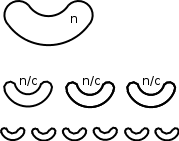
\includegraphics[width=3.5cm,height=2.8cm]{Slike/RekurzivnaCasZahtevnost.png}
% RekurzivnaCasZahtevnost.png: 50.8dpi, width=3.50cm, height=2.80cm, bb=0 0 70 56
	\end{center}
$$
T(n) = 
\left\{
\begin{array}{l}
aT(\frac{n}{c}) + bn^r \mbox{, \v ce je } n>1 \\
b \mbox{, sicer } (n=1)
\end{array} 
\right.
$$
\end{enumerate}

\v Ce velja $a,b,r \geq 0$ in $c > 0$, potem:
\begin{equation}
T(n)=
\left\{
\begin{array}{l}
\Theta (n^r),\; a<c^r \\
\Theta (n^r log n),\; a=c^r \\
\Theta (n^{log_ca}),\; a>c^r
\end{array}
\right.
\label{casovna zahtevnost za rekurzivne algoritme}
\end{equation}

\part{Urejanje}

\section{Urejanje in razvrstitev metod za urejanje}

\paragraph{Pomen:}
\v Ce podatke uredimo jih hitreje najdemo.

\paragraph{Naloga:}
Dani so podatki $a_1, a_2, a_3, \ldots, a_n$.

\paragraph{Cilj:}
Poiskati razporeditev $a_1, a_2, \ldots, a_n$, da bo veljalo $a_1 \leq a_2 \leq \ldots \leq a_{n-1} \leq a_n$.\\
Urejanje lahko razlikujemo po:
\begin{itemize}
	\item vrsti podatkov
	\item relaciji
	\item \v{s}tevilu podatkov
	\item algoritmu
\end{itemize}
Vrsta podatkov:
\begin{enumerate}
	\item $a_i$ so iste dol\v{z}ine:
	\begin{tabular}{ | c | c | c | c | }
		\hline
		$a_1$ & $a_2$ & \ldots & $a_n$\\
		\hline
	\end{tabular}
	\item $a_i$ so razli\v{c}nih dol\v{z}in (uporabimo kazalce):
	\begin{tabular}{ | c | c | c | c | c | }
		\hline
		$a_1$ \hspace{0.1cm} & $a_2$ \hspace{0.05cm} & $a_3$ & $a_4$ \hspace{0.35cm} & \ldots\\
		\hline
	\end{tabular}
\end{enumerate}
Urejanje tukaj pomeni preme\v{s}\v{c}anje (enako dolgih) kazalcev.
\begin{figure}[hbt]
	\centering
	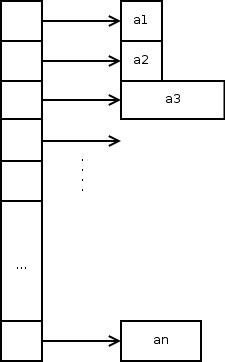
\includegraphics[width=4.45cm,height=7.15cm]{Slike/PoljeKazalcev.png}
% PoljeKazalcev.png: 50.8dpi, width=4.45cm, height=7.15cm, bb=0 0 89 143
	\caption{Polje kazalcev}
	\label{Polje kazalcev}
\end{figure}

\begin{itemize}
	\item velik del programa je neodvisen od vrste podatkov $a_i \Rightarrow$ program je enostavnej\v{s}i
	\item ve\v{c}ja poraba pomnilnika (za tabelo kazalcev )
	\item manj\v{s}a hitrost (ker je pri primerjavi $a_i$ in $a_j$ oba treba dose\v{c}i preko kazalcev)
\end{itemize}


\paragraph*{Relacija $\prec$}

\begin{itemize}
\item definiramo na ve\v{c} na\v{c}inov (procedura \emph{FCmpType} v modulu \emph{sort})
\item definiramo podatka na podlagi katerega se izvaja primerjanje - \underline{klju\v{c}}
\item v praksi je klju\v{c}:
	\begin{itemize}
	\item \v{s}tevilo $\Rightarrow$ relacija $\preceq$ je navadno $\leq$ primerjanje zahteva \underline{konstanten \v{c}as}
	\item \underline{znakovno zaporedje} $\Rightarrow$ relacija $\leq$ je leksikografsko primerjanje, relacija $\leq$ je lahko \v{z}e dana (npr. Oberon - 2) ali pa jo je treba implementirati
	\end{itemize}
\end{itemize}

\begin{figure}[hbt]
	\centering
	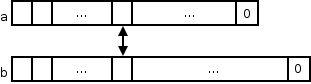
\includegraphics[width=6.1cm,height=1.65cm]{Slike/Primerjanje.png}
% Primerjanje.png: 50.8dpi, width=6.10cm, height=1.65cm, bb=0 0 122 33
	\caption{Primerjanje razli\v cno dolgih tabel}
	\label{Primerjanje}
\end{figure} 


\paragraph{Koda}
\begin{flushleft}
\begin{lstlisting}[language=C, caption={Primer funkcije za primerjanja nizov v jeziku C}]
int CompareStr(char[] a, char[] b)
{
	int i = 0;
	while(a[i] == b[i] && a[i] != 0)
	{
		i++;
	}
	return (int)(a[i] - b[i]);
}
\end{lstlisting}
\end{flushleft}
Primerjanje rabi \underline{spremenljiv \v{c}as}(tudi \v{c}e sta polji enaki).

\paragraph{\v Stevilo podatkov:}
\begin{itemize}
	\item "malo" $\Rightarrow$ vsi podatki so v notranjem pomnilniku v tabeli(array), tak\v{s}no urejanje imenujemo \underline{notranje urejanje}(internal)
	\item "veliko" $\Rightarrow$ vsi podatki so na zunanjem pomnilniku v datoteki(file) $\Rightarrow$ \underline{zunanje urejanje}(external)
	\begin{itemize}
		\item zaporeden dostop do podatkov s pomikanjem datote\v{c}nega okna
		\item vidni so le podatki, ki so v oknu (ti so tudi v notranjem pomnilniku)
		\item v\v{c}asih bomo datoteki rekli trak, da se povdari zaporedni dostop (kot npr. magnetni trak)
	\end{itemize}
\end{itemize}

\subsection{Algoritem}

\begin{itemize}
	\item "navadni" $\Rightarrow$ preprosti in relativno po\v{c}asni
	\item "izbolj\v{s}ani" $\Rightarrow$ bolj zapleteni in relativno hitrej\v{s}i
\end{itemize}
V knjigi so algoritmi napisani v Oberonu.

\paragraph{Algoritmi za urejanje,} ki so si podobni po kak\v{s}ni lastnosti imajo te lastnosti izpostavljene v ustreznem modulu. Najspolo\v{s}nej\v{s}i nalogi ustreza modul:\\
\begin{lstlisting}
MODULE Sort
CONST
	eq*=0; less*=1; grt*=2;
TYPE
	item*=RECORD(*podatkovni element*) END .... ai
	PItem*=POINTER TO item;
	FCmpType*=PROCEDURE(p,q:PItem;r:INTEGER):BOOLEAN;
END Sort;
\end{lstlisting}
\vspace{10pt}
S specializacijo in dedovanjem dobimo module za bolj konkretne naloge:\\
\begin{lstlisting}
MODULE IntSort
IMPORT S:=Sort;
TYPE
       PItem*=POINTER TO Item;
       Item*=RECORD(S.Item) k*:LONGINT END;
END IntSort

MODULE ArrSort
IMPORT I:=IntSort; S:=Sort;
TYPE
      APItem*=ARRAY OF I.PIItem;
      PAPItem*=POINTER TO APItem;
END ArrSort;
\end{lstlisting}

\section{Notranje urejanje}

\paragraph*{Algoritmi za notranje urejanje}

\begin{itemize}
\item \emph{Navadni:}
	\begin{itemize}
	\item potrebuje $\Theta (n^2)$ operacij za ureditev tabele velikosti n
	\item poleg tabel ne rabijo bistveno ve\v{c} prostora
	\item po pristopu:
		\begin{itemize}
		\item navadno vstavljanje (insetion sort)
		\item navadno izbiranje (selection sort)
		\item navadne zamenjave (bubble sort)
		\end{itemize}
	\item imajo enako zgradbo (glej sliko \ref{Diagram navadnega urejanja})
	\begin{figure}[hbt]
		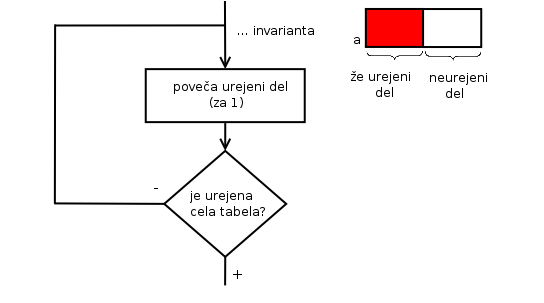
\includegraphics[width=10.7cm,height=5.95cm]{Slike/DiagramUrejanja.png}
		% DiagramUrejanja.png: 50.8dpi, width=10.70cm, height=5.95cm, bb=0 0 214 119
		\caption{Diagram navadnega urejanja}
		\label{Diagram navadnega urejanja}
	\end{figure}
	\item razlikujejo se le po te, kako raz\v{s}irijo urejeni del
	\end{itemize}
\item \emph{Izbolj\v{s}ani:}
	\begin{itemize}
	\item potrebujejo $\Theta (n log n)$
	\item po pristopu:
		\begin{itemize}
		\item Shellovo urejanje (izbolj\v{s}ano vstavljanje)
		\item urejanje s kopico (izbolj\v{s}ano izbiranje) (Heapsort)
		\item urejanje s porazdelitvami (izbolj\v{s}ane zamenjave) (Quicksort)
		\end{itemize}
	\end{itemize}
\end{itemize}
\subsection{Navadno vstavljanje}

\paragraph{Primer}
\begin{flushleft}
\begin{figure}[hbt]
	\centering
	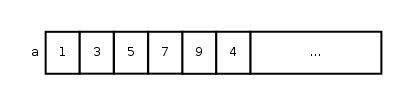
\includegraphics[width=8.15cm,height=1.9cm]{Slike/NavadnoVstavljanjeBinTabela.png}
% NavadnoVstavljanjeBinTabela.png: 50.8dpi, width=8.15cm, height=1.90cm, bb=0 0 163 38
\caption{Primer vhodne tabele pri navadnem vstavljanju}
\end{figure}

\end{flushleft}
\begin{enumerate}
\item zapomnimo si 4
\item vsi ki so v urejenem delu ve\v cji od 4 naj se (eden po eden) premaknejo v desno za eno mesto
\item vstavimo 4 za prvega, ki se ni premaknil
\end{enumerate}

\begin{figure}[h]
	\centering
	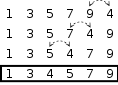
\includegraphics[width=2.3cm,height=1.65cm]{Slike/NavadnoVstavljanjeDemo.png}
% NavadnoVstavljanjeDemo.png: 50.8dpi, width=2.30cm, height=1.65cm, bb=0 0 46 33
	\caption{Primer urejanja z navadnim vstavljanjem}
	\label{Navadno vstavljanje}
\end{figure}


\paragraph{Splo\v sna situacija}
\begin{flushleft}
\begin{figure}[h]
	\centering
	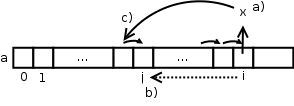
\includegraphics[width=5.8cm,height=2.1cm]{Slike/SplosnaSituacija.png}
% SplosnaSituacija.png: 50.8dpi, width=5.80cm, height=2.10cm, bb=0 0 116 42
	\caption{Prikaz splo\v sne situacije}
\end{figure}
\end{flushleft}

\paragraph{Koda}
Primer metode za algoritem navadnega vstavljanja:\\
\begin{lstlisting}
void InsertionSort(Integer[] a)
{
   int i, j, x;
   int n = a.length();
   for(i=1; i <= n-1; i++)
   {
      j = i;
      x = a[j];
      while((j >= 1) && (x < a[j-1]))
      {
         a[j] = a[j-1];
         j--;
      }
   }
}
\end{lstlisting}

\subsubsection{Uporaba \v cuvaja}
Tabela, ki jo ho\v cemo urediti naj bo sedaj $a[1...n]$, a[i] si bomo zapomnili v a[0] (namesto v x), to je ti. \v cuvaj, da se WHILE zanka ustavi (namesto pogoja $j >= 1$)

\paragraph{Primer}
\begin{center}
	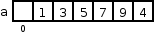
\includegraphics[width=3.05cm,height=0.75cm]{Slike/CuvajPrimer.png}
% CuvajPrimer.png: 50.8dpi, width=3.05cm, height=0.75cm, bb=0 0 61 15
\end{center}

\subsubsection{Psevdokoda}

\begin{flushleft}
\begin{lstlisting}
void SentinelSort(Integer[] a)
{
    int i;
    Integer n = a.length() - 1;   //toliko je elementov, ki jih urejamo

    for(int i=2; i <= n; i++)
    {
        j = i;
        a[0] = a[j];
        while(a[0] < a[j-1])
        {
            a[j] = a[j-1];
            j--;
        }
        a[j] = a[0];
    }
}
\end{lstlisting}
\end{flushleft}

\subsubsection{Analiza \v casa}

\v Cas za ureditev polja $a[1...n]$ je:
\begin{equation}
\begin{array}{rc}
\sum_{i=2}^{n} & \underbrace{\mbox{\v cas za pove\v canje urejenega dela } a[1...i-1]} =\\
 & \mbox{sorazmeren s \v stevilom } C_i\\
 & \mbox{ operacij primerjanja v WHILE}\\
= \sum_{i=2}^{n} C_i &
\end{array}
\end{equation}
$C_i$ je razli\v cen, odvisen od podatkov:
\begin{itemize}
\item $C_{min,i}=1$ ...kadar je a[i] \v ze ve\v cji od vseh v a[1...]
\item $C_{max,i}=i-1$ ...kadar je a[i] manj\v si od vseh v a[1...i-1]
\item $C_{avg,i}=\frac{1}{2}[c_{min,i}+c_{max,i}]$
\end{itemize}
\vspace{10pt}
Od tod dobimo 3 razli\v cne ocene za \v stevilo vseh primerjav:\\
$$
\begin{array}{ll}
C_{min} & = \sum_{i=2}^{n} c_{min,i} = \\
        & = \sum_{i=2}^{n} 1 = \\
        & = n-1 = \\
        & = \Theta(n)\\
C_{max} & = \sum_{i=2}^{n} c_{max,i} = \\
        & = \sum_{i=2}^{n}(i-1) = \\
        & = \frac{1}{2}(n-1)n = \\
        & = \Theta(n^2)\\
C_{ave} & = \sum_{i=2}^{n}C_{ave,i} = \\
        & = \sum_{i=2}^{n}(\frac{1}{2}[c_{min,i}+c_{max,i}] = \\
        & = \frac{1}{2} \sum_{1=2}^{n}[1+i-1] = \\
        & = ... = \\
        & = \frac{1}{4}(n^2+n-2) = \\
        & = \frac{1}{4}(n-1)(n-2) = \\
        & = \Theta(n^2)
\end{array}
$$

\paragraph{Povzetek:}
\begin{itemize}
\item $c_{min}=\Theta(n)$
\item $c_{max}=\Theta(n^2)$  tole nam ni
\item $c_{avg}=\Theta(n^2)$  v\v se\v c!
\end{itemize}
\textbf{Ali lahko algoritem izbolj\v samo?}

\paragraph{Zamisel:}
Ker je $a[1...i-1]$ \v ze urejen, lahko najdemo pravo mesto za $a[i]$ z dvoji\v skim iskanjem.\\
	\begin{center}
	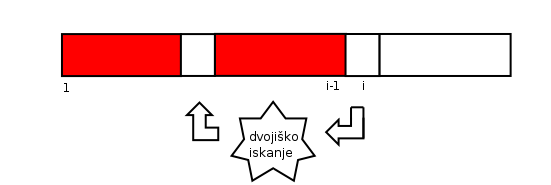
\includegraphics[width=10.85cm,height=3.65cm]{Slike/NavadnoVstavljanjeBinSearch.png}
% NavadnoVstavljanjeBinSearch.png: 50.8dpi, width=10.85cm, height=3.65cm, bb=0 0 217 73
	\end{center}
\begin{equation}
n != \sqrt{2 \pi n}(\frac{n}{e})^n
\label{Stirling}
\end{equation}
\v Stevilo primerjanj je: $C_i=\lceil log_{2}i \rceil$, zato je \v st vseh primerjanj:
$$
\begin{array}{rl}
C & = \sum_{i=2}^n \lceil log_{2}i \rceil \leq \sum_{i=2}^{n} (log_{2}i+1)=\\
  & = logn!+n=\\
  & = log[\sqrt{2\pi n}(\frac{n}{e})^n]+n=\\
  & = log\sqrt{2\pi n}+nlog\frac{n}{e}+n=\\
  & = log\sqrt{2\pi n}+nlogn-nloge+n=\\
  & = \Theta(nlogn)\\
\end{array}
$$

\paragraph{Toda:}
\v Ceprav hitro najdemo pravo mesto za a[i], je \v se vedno treba vse elemente nad $a[i]$ premakniti v desno. To zahteva $\Theta(i)$, zato bo algoritem v celoti \v se vedno reda $\Theta(n^2)$

\paragraph{$\Sigma$:}
Pri analizi je treba paziti, katere operacije zanemarimo, \v se posebej, \v ce nastopajo v zanki

\subsection{Navadno izbiranje (Selection Sort)}

\paragraph{Zamisel:}
	\begin{center}
	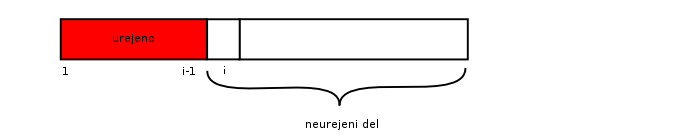
\includegraphics[width=13.75cm,height=2.7cm]{Slike/NavadnoIzbiranjeZamisel.png}
% NavadnoIzbiranjeZamisel.png: 50.8dpi, width=13.75cm, height=2.70cm, bb=0 0 275 54
	\end{center}
Med neurejenimi poi\v s\v ci najmanj\v sega in ga postavi na i-to mesto.

\paragraph{Izvedba:}
Sprehodi se po $a[j], j= i+1,i+2,...,n-1$ in \v ce je $a[j]$ manj\v si pd trenutno najmanj\v sega (ta je v $a[i]$), jih zamenjaj!

\paragraph{Primer:}
	\begin{center}
	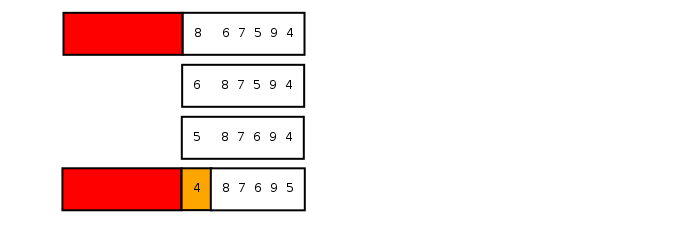
\includegraphics[width=13.75cm,height=4.45cm]{Slike/NavadnoIzbiranjePrimer.png}
% NavadnoIzbiranjePrimer.png: 50.8dpi, width=13.75cm, height=4.45cm, bb=0 0 275 89
	\end{center}

\paragraph{Koda:}
Primer metode za algoritem navadnega izbiranja v Javi:
\begin{lstlisting}
void SelectionSort(Object[] a)
{
	long i, j, n;
	n = a.length();
	for(int i=0; i <= n-2; i++)
	{
		for(int j=i+1; j <= n-1; j++)
		{
			if(a[i] > a[j])
			{
				Exch(a[i], a[j]);
			}
		}
	}
}
\end{lstlisting}

\subsubsection{Analiza \v casa}

\v Stevilo primerjanj:
$$
\begin{array}{ll}
C & = \sum_{i=0}^{n-2}C_{i} = \\
  & = \left / a[i] \mbox{ primerjav z vsemi } a[i+1,i+2,...,n-1] \right / = \\
  & = \sum_{i=0}^{n-2} (n-1-i) = \\
  & = \frac{1}{2} (n-1)n = \\
  & = \Theta (n^2)
\end{array}
$$
C je neodvisen od podatkov, ker se $a[i]$ primerja z vsemi.\\
\\
\textbf{Kaj pa \v stevilo zamenjav?}\\
\\
Naj bo $M_{i}$ \v stevilo zamenjav z $a[i]$:
\begin{itemize}
\item $M_{min,i}=0$ (ko je $a[i]$ \v ze najmanj\v si med neurejenimi)
\item $M_{max,i}=n-1-i$ (ko je $a[i]$ najve\v cji med neurejenimi)
\end{itemize}
Od tod sledi:
$$
\begin{array}{l}
M_{min}=\sum_{i=0}^{n-2} M_{min,i}=0\\
M_{max}=\sum_{i=0}^{n-2} M_{max,i}=\sum(n-1-i)=\frac{1}{2} (n-1)n=\Theta (n^2)
\end{array}
$$

\subsection{Navadne zamenjave (Bubble Sort)}

\paragraph{Primer:}
	\begin{center}
	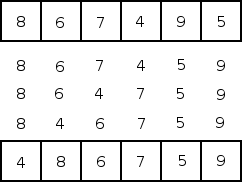
\includegraphics[width=4.75cm,height=3.6cm]{Slike/NavadneZamenjavePrimer.png}
% NavadneZamenjavePrimer.png: 50.8dpi, width=4.75cm, height=3.60cm, bb=0 0 95 72
	\end{center}

\paragraph{1. sprehod:}
Sprehodimo se od desne v levo po neurejenem delu pri vsakem koraku primerjamo soseda in ju zamenjamo, \v ce je potrebno.\\
Po 1. sprehodu je $a[0]$ urejen del tabele in vsebuje najanj\v si element celotne tabele.

\paragraph{Splo\v sno:}
\begin{itemize}
\item \textbf{predpostavka:} po i-tem sprehodu je a[0...i-1] urejen del in vsebuje i najmanj\v sih elementov (celotne) tabele\\
	\begin{center}
	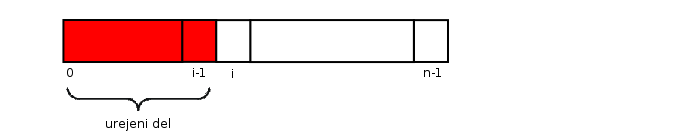
\includegraphics[width=13.75cm,height=2.7cm]{Slike/NavadneZamenjaveSplosno.png}
% NavadneZamenjaveSplosno.png: 50.8dpi, width=13.75cm, height=2.70cm, bb=0 0 275 54
	\end{center}
\item sedaj se sprehodimo po neurejenem delu, od desne v levo, po indeksih $j=n-1,...,i$, pri \v cemer $a[j-1]$ in $a[j]$ zamenjamo, \v ce je treba
\item ko se sprehod kon\v ca je v a[i] najmanj\v si element neurejenega dela
\item $a[i]$ je ve\v cji (ali enak) od vseh elementov v urejenem delu
\item \textbf{posledica:} $a[0...i]$ urejen del tabele, vsebuje i+1 najmanj,\v sih elementov celotne tabele (zan\v cna invarianta)\\
\v ce to ponavljamo od $i=1$ do $n-1$ bo tabela urejena
\end{itemize}

% od Salesky
\paragraph{Koda:}
\begin{flushleft}
\begin{lstlisting}[caption={BubbleSort}, language={Java}]
void BubbleSort(Comparable[] a)
{
   int n = a.length;
   for(int i = 1; i < n; i++)
   {
      for(int j = n-1; j >= i; j--)
      {
         if(a[j-1].CompareTo(a[j]) == 1)
         {
            Zamenjaj(a[j-1], a[j]);
         }
      }
   }
}
\end{lstlisting}
\end{flushleft}

\paragraph{Analiza}
\begin{list}{}{}
\item V 1. sprehodu je n-1 primerjanj.
\item V 2. sprehodu je n-2 primerjanj.
\item ...
\item V n-1 sprehodu je 1 primerjanje.
\end{list}
Vseh primerjanj je : $1+2+...+n-1 = ½(n-1)n = \Theta(n^2)$\\
Poskusimo \v se izbolj\v sati algoritem sortiranja.

\subsection{Izmeni\v cne zamenjave (shaker sort)}

\paragraph{Opazimo:}
Naj bo najmanj\v si element v neurejenem delu tabele, kjer ka\v ze pu\v s\v cica.

	\begin{center}
	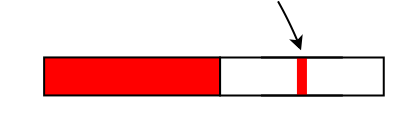
\includegraphics[width=8.05cm,height=2.3cm]{Slike/IzmenicneZamenjaveTabela.png}
% IzmenicneZamenjaveTabela.png: 50.8dpi, width=8.05cm, height=2.30cm, bb=0 0 161 46
	\end{center}

Ko ga sprehod v levo dose\v ze, ga »zagrabi« in odnes s seboj do levega roba. \\

\begin{flushleft}
\textbf{Kaj pa se dogaja z najve\v cjim elementom neurejenega dela?} \\
Vsak sprehod gre \v cezenj, ob vsakem sprehodu se pomika v desno.
\end{flushleft}


\paragraph{Zamisel:}
Uvedemo \v se sprehode v desno, sprehod v desno bo zagrabil najve\v cjega v neurejenem delu tabele in ga premaknil na desni rob. V vsakem trenutku bosta \textbf{dva} urejena dela tabele:
	\begin{center}
	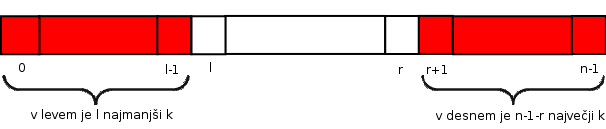
\includegraphics[width=11.95cm,height=2.55cm]{Slike/ShakerSortTabela.png}
% ShakerSortTabela.png: 50.8dpi, width=11.95cm, height=2.55cm, bb=0 0 239 51
	\end{center}
Izmeni\v cno se sprehajamo po neurejenem delu $a[l..r]$ v levo in desno in potisnemo najmanj\v si oz. najve\v cji element na levi oz. na desni rob (najmanj\v si pristane v a[l], najve\v cji pa v a[r] $\Rightarrow$ levi rob se pomakne v desno za 1, desni pa v levo za 1.

\paragraph{\v Se ena zamisel:}
\v Ce se pri sprehodu v levo zadnja zamenjava zgodi med $a[i-1]$ in $a[i]$, so po sprehodu o\v citno $a[0...i]$ urejeni, zato lahko levo rob »presko\v ci« na $i+1$.
podobno tudi pri desnemu sprehodu
vse skupaj kon\v camo, ko postane $l>r$.

\begin{lstlisting}[caption={Algoritem za sortiranje z izmeni\v cnimi zamenjavami}]
void ShakerSort(Comparable[] a)
{
   int i, j, n, l, r;
   n = a.length;
   l = 1;
   r = n-1;
   i = n-1;
   do
   {
      for(j = r; j >= l; j--)
      {
         if(a[j-1].CompareTo(a[j]) == 1)
         {
            Zamenjaj(a[j-1],a[j]);
            i = j;
         }
      }
      l = i + 1;
      for(j = l; j <= r; j++)
      {
         if(a[j-1].CompareTo(a[j]) == 1)
         {
            Zamenjaj(a[j-1], a[j]);
            i = j;
         }
      }
      r = i-1;
   }
   while(l > r);
}
\end{lstlisting}

\paragraph{Pri\v cakujemo:}
\begin{itemize}
\item pri\v cakujemo bolj\v si povpre\v cni \v cas zaradi druge zamisli
\item v najslab\v sem primeru \v se vedno $\Theta (n^2)$
\end{itemize}

\paragraph{Navadni algoritmi} za notranje sortiranje:
\begin{itemize}
	\item navadno vstavljanje
	\item navadno izbiranje
	\item navadne zamenjave
\end{itemize}
Vsi zahtevajo $\Theta(n^2)$ \v casa (merjeno v operacijah primerjanja ali zamenjav).\\
\\
\textbf{Ali se da zabele urediti hitreje, npr. v \v casu $\Theta(n)$ ali $\Theta(\sqrt{n})$ ali $\Theta(logn)$?}\\
Ocenimo, najmanj koliko je potrebnih operacij primerjanja.\\
\\
\textbf{Kako urediti n.danih \v st., \v ce je na voljo le operacija primerjanja?}

\paragraph{Primer:}
Dana so \v st. a, b in c, ki so razli\v cna.\\
Naloga: Kako so urejena po vrsti?\\
Uporabimo algoritem, ki ga predstavlja naslednji diagram poteka.
\begin{figure}[h]
	\centering
	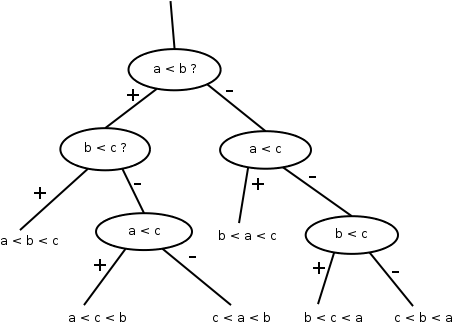
\includegraphics[width=8.9cm,height=6.5cm]{Slike/DvojiskoDrevoUrejanja.png}
% DvojiskoDrevoUrejanja.png: 50.8dpi, width=8.90cm, height=6.50cm, bb=0 0 178 130
	\caption{Diagram poteka}
\end{figure}
Diagram poteka je dvoji\v sko drevo, ki ima v notranjih vozli\v s\v cih primerjanja, v listih pa vse mo\v zne ugotovitve (vse mo\v zne ureditve \v st. a,b in c v permutacije).

\paragraph{Splo\v sno:}
\v Ce so dana \v st. a1, a2, a3,... an, lahko njihovo urejenost ugotovimo z vsakim diagramom poteka, ki ima obliko dvoji\v skega drevesa, ki ima v notranjih vozli\v s\v cih primerjanja, v listih pa vse mo\v zne permutacije \v stevil a1, a2,..., an.\\
\\
\v Ce med izvajanjem algoritma pridemo do vsakega lista, izvemo kako so urejeni vhodni a1, a2,..., an.\\
\\
Opisano drevo ima n! listov (po en list za vsako permutacijo \v st. a1, a2,..., an). Vsako dvoji\v sko drevo z N listi ima vi\v sino $\geq log2 N$. Opisano drevo ima vi\v sino $\geq log2 N!$
\begin{figure}[h]
	\centering
	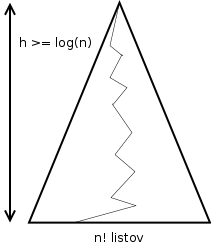
\includegraphics[width=4.15cm,height=4.9cm]{Slike/VisinaDrevesaSkica.png}
% VisinaDrevesaSkica.png: 50.8dpi, width=4.15cm, height=4.90cm, bb=0 0 83 98
	\caption{Vi\v sina drevesa}
\end{figure}
Pri urejanju n elementov $a_1, a_2,... a_n$ bo potrebnih $\geq log_2 n!$ primerjanj.\\
\\
\v Stevilo primerjanj:
$$
\begin{array}{ll}
\mbox{\v st. primerjanj} & \geq log_2 n! \doteq \\
 & = /* \mbox{po Stirlingu } n! \doteq \sqrt{2\Pi n} \left( \frac{n}{e} \right) ^n */ = \\
 & = log\sqrt{2\Pi n} \left( \frac{n}{e} \right) ^n = \\
 & = ... = \\
 & = n log n - \frac{1}{2}log n - 1.44n \geq \\
 & \geq c n log n = \\
 & = \Theta (n log n)
\end{array}
$$
Vsak algoritem za urejanje n \v stevil zahteva vsaj $c n log n$ operacij primerjanja (za ureditev vsaj enega vhoda). Torej je smiselno iskati algoritme, ki rabijo $\Theta (n log n)$ \v casa!

\subsection{Shellovo urejanje (izbolj\v sano vstavljanje)}

\paragraph{Motivacija}
Pri navadnem vstavljanju je a[i] primerjanj z vsemi, ki so v urejenem delu in so ve\v cji od njega (pri tem so vsi ki so ve\v cji od njega pomikajo v desno).

\paragraph{Shellova zamisel}
a[i] naj se primerja z elementi na levi po vrsti ampak z vsakim h-tim (npr. h=3). Sedaj se ti pomikajo desno toda za h mest, \v ce so ve\v cji od a[i], a[i] pa gre na mesto tistega, ki se je prestavil zadnji.
	\begin{center}
	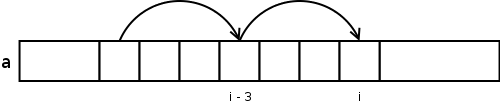
\includegraphics[width=9.85cm,height=2.15cm]{Slike/ShellovoUrejanje1.png}
% ShellovoUrejanje1.png: 50.8dpi, width=9.85cm, height=2.15cm, bb=0 0 197 43
	\end{center}
Tako da bo a[i] hitreje (z manj primerjanji) pri\v sel v levo.\\
\\
\textbf{Ali se urejenost urejenega (levega) dela ne poru\v si, ko nekateri elementi preskakujejo druge?}

\paragraph{Odgovor}
Ne, \v ce ne zahtevamo ve\v c, da je osen\v cen del v celoti urejen, temve\v c, da je sestavljen iz ve\v c podtabel od katerih je vsaka zase urejena.\\
\\
Npr.: podtabelo a sestavljajo elementi:
	\begin{center}
	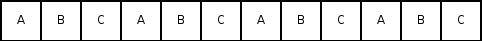
\includegraphics[width=9.5cm,height=0.8cm]{Slike/ShellovoUrejanje2.png}
% ShellovoUrejanje2.png: 50.8dpi, width=9.50cm, height=0.80cm, bb=0 0 190 16
	\end{center}

\paragraph{Shellov algoritem}
Neurejeno tabelo razdeli na ve\v c porazdeljenih podtabel (A, B, C). Vsako podtabelo uredi z navadnim vstavljanjem. Ko so vse podtabele urejene (vsaka zase), vse skupaj ponovi z manj\v sim \v stevilom podtabel. Algoritem se kon\v ca , ko je \v st podtabel enako 1.

\paragraph{Primer:}
\begin{figure}[hbt]
	\centering
	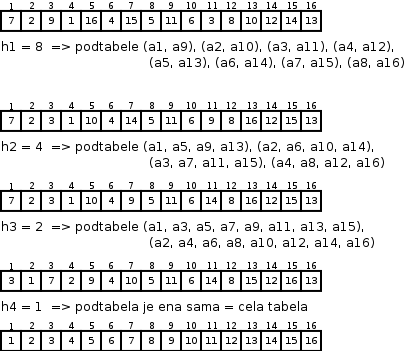
\includegraphics[width=7.95cm,height=6.9cm]{Slike/ShellovoUrejanjePrimer.png}
% ShellovoUrejanjePrimer.png: 50.8dpi, width=7.95cm, height=6.90cm, bb=0 0 159 138
	\label{Primer urejanja s Shellovo metodo}
\end{figure}

\paragraph{Vpra\v sanje:}
\textbf{Kak\v sno naj bo zaporedje?}\\
V prej\v snjem primeru:
$$
\begin{array}{l}
h_1 = 8 \\
h_2 = 4 \\
h_3 = 2 \\
h_4 = 1 \mbox{, torej } t = 4
\end{array}
$$

\paragraph{Odgovor:} Va\v zno je, da za zaporedje velja: 
$$h_1 > h_2 > h_3 > ... > h_{t-1} > h_t = 1.$$
Toda nekatera zaporedja so bolj ugodna od drugih (dokazano z eksperimenti), npr.:
\begin{enumerate}
\item ...121 40 13 4 1... $h_{n-1} = 3h_n + 1, h_t = 1$
\item ...31 15 7 3 1... $h_{n-1} = 2h_n + 1, h_t = 1$
\end{enumerate}
\textbf{Kateri od njih naj bo za\v cetni h ($h_1$) oz. koliko je t?}
\begin{enumerate}
\item $t = \lfloor log_3 n \rfloor - 1$
\item $t = \lfloor log_2 n \rfloor - 1$
\end{enumerate}

\paragraph{Analiza:} Glej knjigo Knuth D.: TAOCP \cite{knuth98}\\
Shellovo urejanje ima pri zaporedju:
\begin{enumerate}
\item \v casovno zahtevnost $\Theta (n^{1.5})$
\item \v casovno zahtevnost $\Theta (n^{1.26})$
\end{enumerate}

\paragraph{Pozor:} $n^{1.26}$ je \v se vedno asimptoti\v cno gledano ve\v cja funkcija kot $n log n$.

\subsection{Urejanje s kopico}

\subsection{Motivacija}

Pri pregledu neurejenega dela bi bilo treba nabrati ve\v c koristnih informacij in jih uporabit. Navadna urejanja "nimajo spomina".

\paragraph{Kako?} Neurejeni elementi naj bodo v kopici.

\subsection{Kopica (heap)}

\begin{itemize}
\item je dvoji\v sko drevo (vozli\v s\v ca hranijo elemente a[1], a[2], ... ,a[n]  oz. njihove klju\v ce)
\item ki je urejeno da za vsako vozi\v s\v ce velja, da je ve\v cje od vseh elementov v njegovih dveh poddrevesih (\v ce obstajata)
\item je levo uravnote\v zeno – vse veje drevesa so dolge d ali d-1 (za nek d) in vse dalj\v se veje do zbrane na levi strani
\end{itemize}

\paragraph{Primer:}
\begin{figure}[hbt]
	\centering
	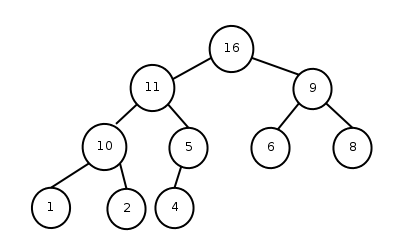
\includegraphics[width=7.75cm,height=4.9cm]{Slike/KopicaPrimer.png}
% KopicaPrimer.png: 50.8dpi, width=7.75cm, height=4.90cm, bb=0 0 155 98
	\caption{Primer kopice}
\end{figure}

\paragraph{Opazimo:}
\begin{itemize}
\item klju\v ci vzdol\v z poljubne veje so urejeni, npr:
	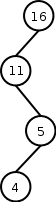
\includegraphics[width=1.1cm,height=4cm]{Slike/KopicaVeja.png}
% KopicaVeja.png: 50.8dpi, width=1.10cm, height=4.00cm, bb=0 0 22 80
\item najve\v cji klju\v c je v korenu drevesa
\item \v ce je drevo 
	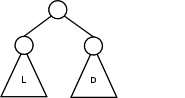
\includegraphics[width=3.65cm,height=1.95cm]{Slike/KopicaSPoddrevesi.png}
% KopicaSPoddrevesi.png: 50.8dpi, width=3.65cm, height=1.95cm, bb=0 0 73 39
	kopica, sta kopici tudi levo in desno poddrevo
	\begin{figure}[hbt]
		\centering
		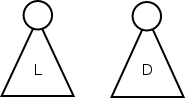
\includegraphics[width=3.65cm,height=1.95cm]{Slike/LevoInDesnoPoddrevo.png}
	% LevoInDesnoPoddrevo.png: 50.8dpi, width=3.65cm, height=1.95cm, bb=0 0 73 39
		\caption{Levo in desno poddrevo}
	\end{figure}
\end{itemize}

\subsubsection{Uporaba pri urejanju}

\begin{enumerate}
\item izlo\v ci koren in ga nekam shrani %\label{Izlo\v ci koren}
\item namesto njega postavi zadnji list %\label{Dvigni zadnjega}
\item popravi dobljeno drevo v kopico (koren se pogrezne tja kamor sodi s tem da se zamenjuje z ve\v cjim od sinov)
\end{enumerate}
Izlo\v ceni koreni so urejeni po velikosti.

\paragraph{Primer}
\begin{flushleft}
po 1)... do 2): \\
	\begin{center}
	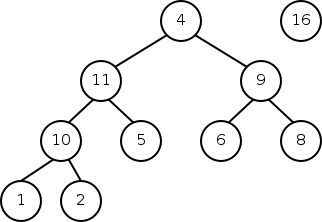
\includegraphics[width=6.36cm,height=4.35cm]{Slike/KopicaUrejanje1.png}
% KopicaUrejanje1.png: 50.8dpi, width=6.35cm, height=4.35cm, bb=0 0 127 87
	\end{center}
pogrezanje 4:
	\begin{center}
	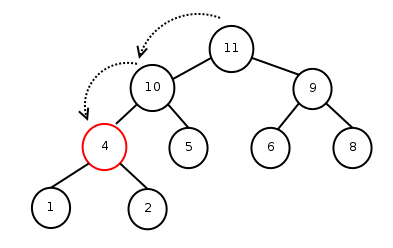
\includegraphics[width=7.75cm,height=4.9cm]{Slike/Pogrezanje4}
% Pogrezanje4.: 50.8dpi, width=7.75cm, height=4.90cm, bb=0 0 155 98
	\end{center}
ponovimo 1)...2) (izlo\v cimo 11):
	\begin{center}
	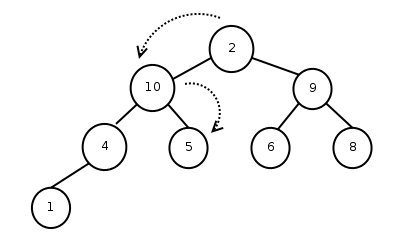
\includegraphics[width=7.75cm,height=4.9cm]{Slike/PokvarjenaKopica}
% PokvarjenaKopica.png: 50.8dpi, width=7.75cm, height=4.90cm, bb=0 0 155 98
	\end{center}
in popravimo kopico:
	\begin{center}
	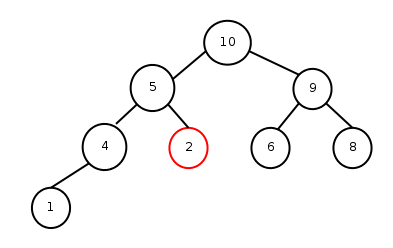
\includegraphics[width=7.75cm,height=4.9cm]{Slike/Pogrezanje2}
% Pogrezanje2.png: 50.8dpi, width=7.75cm, height=4.90cm, bb=0 0 155 98
	\end{center}
\end{flushleft}
Popravljamo dokler ne izpraznimo kopice.

\paragraph{Podatkovna struktura:}

\begin{itemize}
\item kopico realiziramo s tabelo a 
	\begin{center}
	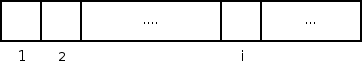
\includegraphics[width=7.15cm,height=1.4cm]{Slike/RealizacijaKopiceSTabelo.png}
% RealizacijaKopiceSTabelo.png: 50.8dpi, width=7.15cm, height=1.40cm, bb=0 0 143 28
	\end{center}
	kjer:
	\begin{itemize}
	\item koren kopice je v a[1]
	\item \v ce je neko vozli\v s\v ce kopice v a[i], sta levi in desni sin (\v ce obstajata) shranjena v a[2i] in a[2i + 1]
	\end{itemize}
\end{itemize}

\paragraph{Primer}

	\begin{center}
	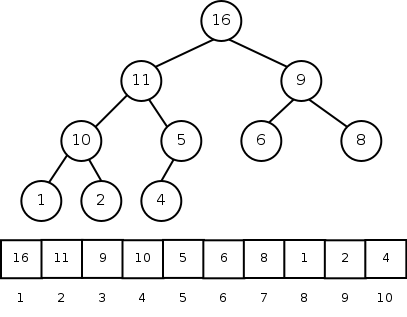
\includegraphics[width=8cm,height=6.25cm]{Slike/PrimerKopice.png}
% PrimerKopice.png: 50.8dpi, width=8.00cm, height=6.25cm, bb=0 0 160 125
	\end{center}
Torej:
\begin{itemize}
\item \v ce je $s > 1$, je $a[s]$ sin nekoga
\item njegov o\v ce je v celici $a[s/2]$
\item s sodo \v st. $\Rightarrow a[s]$ je levi sin
\item z liho \v st. $\Rightarrow a[s]$ je desni sin
\end{itemize}

\paragraph{Urejanje:}
\begin{center}
	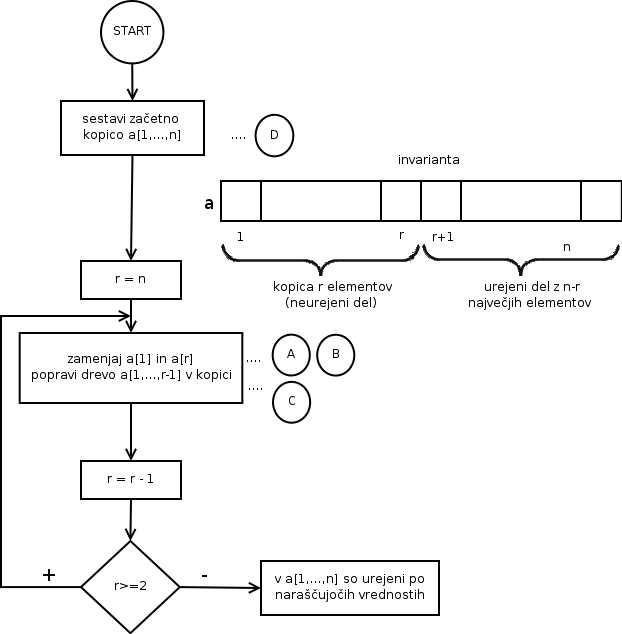
\includegraphics[width=12.25cm,height=12.5cm]{Slike/HeapSortDiagram.png}
% HeapSortDiagram.png: 50.8dpi, width=12.25cm, height=12.50cm, bb=0 0 245 250
\end{center}
Urejanje poteka na mestu (in situ), kar je ugodno.\\
\\
\textbf{Kako izvesti korak C in D?}\\
\\
Denimo, da bi imeli na voljo proceduro PopraviVKopico(i,j), ki bi znala drevo popraviti v kopico ob predpostavki, da sta obe poddrevesi vozli\v s\v ca \v ze kopici.
	\begin{center}
	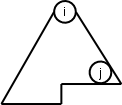
\includegraphics[width=2.4cm,height=2.05cm]{Slike/Poddrevo.png}
% Poddrevo.png: 50.8dpi, width=2.40cm, height=2.05cm, bb=0 0 48 41
	\end{center}
Tedaj bi bil C kar klic PopraviVKopico(1,r-1).\\
Sestavljanje za\v cetne kopice bi za\v celi od zadnjega o\v ceta (ker so listi \v ze kopice) po nivojih navzgor do korena, pri \v cemer pri vsakem vozli\v s\v cu pokli\v cemo proceduro PopraviVKopico.
	\begin{center}
	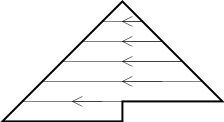
\includegraphics[width=4.4cm,height=2.4cm]{Slike/SestaviZacetnoKopico.png}
% SestaviZacetnoKopico.png: 50.8dpi, width=4.40cm, height=2.40cm, bb=0 0 88 48
	\end{center}
Torej je D:
\begin{lstlisting}[language={c}]
void SestaviZacetnoKopico()
{
	int i;
	for(i = n/2; i > 0; i--)
	{
		PopraviKopico(i, n);
	}
}
\end{lstlisting}
\textbf{Kak\v sna je PopraviVKopico(i,j)?}
\begin{itemize}
\item poglejmo poddrevo
	\begin{center}
	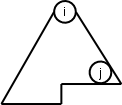
\includegraphics[width=2.4cm,height=2.05cm]{Slike/Poddrevo.png}
% Poddrevo.png: 50.8dpi, width=2.40cm, height=2.05cm, bb=0 0 48 41
	\end{center}
\item \v ce je i list, je \v ze (trivialna) kopica
\item \v ce ni list, ima vsaj enega sina: vozli\v s\v ce $s = 2i$, \v ce je $s + 1 \leq j$, pa tudi desnega 
\item predpostavimo, da sta L in D obe kopici
	\begin{center}
	\includegraphics[width=3.9cm,height=3.45cm]{Slike/KopicaLD.png}
% KopicaLD.png: 50.8dpi, width=3.90cm, height=3.45cm, bb=0 0 78 69
	\end{center}
\item pozornost usmerimo na ve\v cjega od sinov (denimo da bo to sin z indeksom s)
\item poddrevo, kjer je sedaj o\v ce, je morda treba spet popraviti v kopico, zato zopet pokli\v cemo proceduro PopraviVKopico (rekurzija)
\end{itemize}

\begin{lstlisting}[language={c}]
void PopraviVKopico(int i, int j)
{
   int s;
   if (i <= j/2) .... i ima sina
   {
      s = 2*i;	//s je levi
      if ((s+1) <= j)	//ce obstaja desni sin
      {
         if (a[s] < a[s+1])
         {
            s++;	//naj s oznacuje vecjega
         }
      }
      if (a[i] < a[s])
      {
         Zamenjaj(a[i], a[s])	//zamenjaj
         PopraviVKopico(s, j)	/* popravi se drevo
				   kamor je prisel oce */
      }
   }
}
\end{lstlisting}

\subsubsection{Celoten algoritem za heapsort}

\begin{lstlisting}[language={c}]
void HeapSort(int[] a)
{
	int r;
	SestaviZacetnoKopico();
	for (int i=n; i >= 2; i--)
	{
		Zamenjaj(a[i], a[r]);
		PopraviVKopico(1, r-1);
	}
}
\end{lstlisting}

\subsubsection{Analiza}

\begin{itemize}
\item PopraviVKopico(i,j):
	\begin{itemize}
	\item primerja in zamenjuje vozli\v s\v ca vzdol\v z ene veje, zato rabi $T(i) = \Theta (k(i))$ operacij, kjer je k(i) vi\v sina vozli\v s\v ca i, tj.  $h(i) = log2$(\v st. elementov v poddrevesu vozli\v s\v ca i)
	\end{itemize}
\item SestaviVKopico:
	\begin{itemize}
	\item kli\v ce PopraviVKopico v zanki, zato rabi
	\item velja: to je reda $\Theta (n)$
	\item dokaz: na vi\v sini k je kve\v cjemu $\lceil \frac{n}{2^k} \rceil$ vozli\v s\v c, zato:
	$$
	\begin{array}{rl}
	\sum_{i=\lfloor \frac{n}{2} \rfloor}^2 & = \left / \mbox{se\v stevamo po vi\v sinah} \right / \\
	& = \sum_{k=1}^h (\frac{n}{2^k}k) = \\
	& = n \underbrace{\sum_{k=1}^h (\frac{k}{2^k})} = \\
	& \mbox{konvergira ko gre } h \rightarrow \infty \\
	& = n \cdot \mbox{konst.} = \\
	& = \Theta (n)
	\end{array}
	$$
	\end{itemize}
	\begin{center}
	\includegraphics[width=4.3cm,height=4.15cm]{Slike/CasovnaZahtevnostKopica.png}
% CasovnaZahtevnostKopica.png: 50.8dpi, width=4.30cm, height=4.15cm, bb=0 0 86 83
	\end{center}
\item Heapsort:
	\begin{itemize}
	\item SestaviVKopico ...... $\Theta (n)$
	\item zanka rabi:
	$$
	\begin{array}{rl}
	\sum_{r=n}^2 (1 + T(r-1)) & = \sum_{r=1}^{n-1} (1 + T(r)) = \\
	& \leq n - 1 + \sum_{r=1}^{n-1} T(r) \\
	& \leq n - 1 + \sum_{r=1}^{n-1} log_2(r) = \\
	& n - 1 + log_2(n-1)! = \\
	& \left / \mbox{Stirling} \right / \\
	& \leq n - 1 + log_2(\sqrt{2 \Pi (n-1)} (\frac{n-1}{e})^{n-1}) \leq \\
	& \leq ... nlogn = \\
	& = \Theta (n log n)
	\end{array}
	$$
	\item algoritem je asimptoti\v cno optimalen glede \v stevila primerjanj
	\end{itemize}
\end{itemize}

\subsection{Urejenje s porazdelitvami (Quicksort)}

\paragraph{Motivacija}
Pri metodi navadnih zamenjav se sprehajamo od leve proti desni in menjavamo sosednja elementa. Primer: a[1, 2, 99, 98,...81, 80, 3, 100]. Opazimo, da bo potrebnih bo veliko zamenjav, da bo 3 pri\v sla na svoje mesto!\\
\\
\textbf{Zakaj kar takoj ne zamenjamo te 3 in 99?}

\paragraph{Zamisel}
Mo\v zne naj bodo zamenjave med poljubno oddaljenimi elementi.\\
\\
\textbf{Kako mo\v znost oddaljenih zamenjav \v cimbolj izkoristiti?}

\paragraph{Zamisel}
\begin{enumerate}
\item Tabelo z oddaljenimi zamenjavami na grobo uredimo glede na neko mejno vrednost m, tj. elemente tabele a porazdelimo (preme\v cemo) v tri podtabele t1, t2, t3, kjer:
	\begin{center}
	\includegraphics[width=6.7cm,height=1.2cm]{Slike/QuickSortTabela1.png}
% QuickSortTabela1.png: 50.8dpi, width=6.70cm, height=1.20cm, bb=0 0 134 24
	\end{center}
\item Potem na podoben na\v cin uredimo t1 in t3 (na mestu), npr. z rekurzivnim klicem iste procedure (rekurzivni razcep)
\end{enumerate}

\subsubsection{Koda}

\begin{lstlisting}
void Quicksort(t)
{
	if(t.length==1)
		return t;
	else
	{
		m = izberi med elementi tabele t;
		porazdeli tabelo t v podtabele t1, 
		  t2 in t3 glede na m;
		return(Quicksort(t1); t2; Quicksort(t3));
	}
}
\end{lstlisting}

\vspace{10pt}
\paragraph{Opombe}
Algoritem kli\v ce sebe (rekurzivno) dvakrat (rekurziven razcep).
\begin{enumerate}
\item \textbf{Kako (hitro) izbrati m?}\\
V konstantnem \v casu ($\Theta (1)$) so mo\v znosti:
\begin{itemize}
	\item npr. m = prvi element tabele (lahko slabo), ker je lahko $|t1|<<|t3|$
	\item m je srednji element v tabeli (kot npr. v knjigi prof. Vilfana \cite{vilfan02})
	\item m je naklju\v cno izbrani ($\Rightarrow$ uporabiti je treba generator naklju\v cnih \v stevil $\Rightarrow$ izguba \v casa)
	\item m = 1/3 (prvi, srednji, zadnji)
\end{itemize}
Najbolje je, \v ce sta t1 in t3 (pribli\v zno) enako dolga, toda v \v casu $\Theta (1)$ ne moremo najti m, ki bi to zagotovljal.
\item \textbf{Kako (hitro) porazdeliti tabelo t v podtabele t1, t2 in t3 (glede na m)?} \\
	\begin{enumerate}
	\item \textbf{Prva mo\v znost:} \\
		najprej iz t[] sestavimo $[t1, t2 \cup t3]$, nato iz tega $[t1, t2, t3]$
	\item \textbf{Druga mo\v znost:} \\
		Ostanemo pri $[t1, t2 \cup t3]$ (tj. prihranimo si iskanje meje med t2 in t3), v glavnem programu pa kli\v cemo:
		\begin{verbatim}
		return(Quicksort(t1); Quicksort(t2 u t3))
		\end{verbatim}
	\end{enumerate}
\end{enumerate}

\paragraph{Zamisel:}
Z indeksoma i in j se sprehodimo od levega in desnega roba tabele, dokler ne najdemo dveh elementov, ki sodita v nasprotno podtabelo, elementa zamenjamo in nadaljujemo sprehod.

\begin{center}
	\includegraphics[width=10.2cm,height=1.95cm]{Slike/QuickSortTabela2.png}
% QuickSortTabela2.png: 50.8dpi, width=10.20cm, height=1.95cm, bb=0 0 204 39
\end{center}

\begin{lstlisting}[language=c, caption={Primer metode, ki razdeli elemente v podtabele}]
void Partition(t, p, z, m)
{
	 int i, j;
	 i=p;
	 j=z;
	 while(i<j)
	 {
		 while(t[i]<m && i<=z)
			 i++;
		 while(t[j]>=m && j>=p)
			 j--;
		 if(i<j)
		 {
			 zamenjaj(i, j);
			 i++;
			 j--;
		 }
	 }
}
\end{lstlisting}

\paragraph{Opomba}
Ko se partition kon\v ca, je t1 v $t[p,...,i-1]$ in $t2 \cup t3$ v $t[j+1,...,z]$. $Partition(t,...)$ zahteva $\Theta (|t|)$ operacij primerjanja in $\pm$.

\begin{lstlisting}[language=c, caption={Celoten algoritem za hitro sortiranje}]
void Quicksort(t)
{
	if(t ima en element)
	{
		return t;
	}
	else
	{
		m = izberi med elementi tabele t;
		porazdeli t na t1 in (t2 unija t3);
		return(Quicksort(t1); Quicksort(t2 u t3));
	}
}
\end{lstlisting}
Naj bo $T(|t|)$ \v cas za ureditev tabele t, tedaj:
	\begin{equation}
	T(|t|) = T(|t1|) + T(|t2 \cup t3|) + \Theta (|t|)+ \Theta (1)
	\label{Porazdelitev}
	\end{equation}
Re\v sitev te en\v cbe je odvisna od tega, kako uravnote\v zeno je porazdeljevanje.\\

\paragraph{Najslab\v si \v cas}
Naj bo vsaka porazdelitev (na vsakem koraku algoritma) maksimalno neuravnote\v zena, tj. da razdelitev vrne:
	$$t[t1, t2 \cup t3]$$
Ena\v cba (\ref{Porazdelitev}) se glasi:
$$
\begin{array}{c}
T_{max}(n) = T_{max}(1) + T_{max}(n-1) + \Theta (n) + \Theta (1) \mbox{, oziroma} \\
T_{max}(n)=T_{max}(n-1) + \Theta (n)
\end{array}
$$
Ra\v cunamo:
$$
\begin{array}{ll}
Tmax(n) & = /*razvijemo*/ = \\
 & = \Theta (1)+\Theta (2)+...+\Theta (n) = \\
 & = \sum_{h=1}^n (\Theta (h)) = \\
 & = \Theta (vsota[1, n](h)) = \\
 & = \Theta (n^2)
\end{array}
$$

\paragraph{Najbolj\v si \v cas}
Predpostavimo naj bo porazdelitev najbolj uravnote\v zena kar se le da (na vsakem koraku algoritma), tj. vrne porazdelitev na sve enako dolgi podtabeli:
$$t[t1, t2 \cup t3].$$
Ena\v cba (\ref{Porazdelitev}) je torej:
$$T_{min}(n)=T_{min}(n/2) + T_{min}(n/2) + \Theta (n)+\Theta (1) \mbox{ oziroma}$$
$$T_{min}(n)=2 * T_{min}(n/2) + \Theta (n)$$
Ta ena\v cba je oblike:
$$
T(n)=a * T(n/c) + b*n^r =
\left\lbrace 
\begin{array}{l}
\Theta (n^r); \mbox{ \v ce } a<c^r \\
\Theta (n^r*log(n)); \mbox{ \v ce } a=c^r \\
\Theta (n*log_c(a)); \mbox{ \v ce } a>c^r \\
\end{array}
\right.
$$
Pri nas:
$$
a=c=2
r=1
$$
Re\v sitev: $T_{min}(n) = \Theta (n*log(n))$\\
\\
\textbf{Kaj pa v povpre\v cju?}

\paragraph{Povpre\v cen \v cas}
Predpostavimo, da so vsi elementi tabele razli\v cni.\\
Posledica:
\begin{itemize}
\item tabela $t_1$ in $t_3$ karseda veliki (ker je v $t_2$ kve\v cjemu en element)
\item s tem bo tudi povpre\v cen \v cas karseda velik (pesimisti\v cen) $\Rightarrow$ analiza ne bo preve\v c optimisti\v cna
\end{itemize}
Naj bo $T_{avr}(n)$ povpre\v cen \v cas za ureditev n elementov tabele t. Velja:
$$
T_{avr}(0) = T_{avr}(1) = b = \Theta (1)
$$
Naj bo m, ki ga izbiramo i-ti ($i = 1,2,... n$) najmanj\v si v tabeli, torej:
	\begin{center}
	\includegraphics[width=11.65cm,height=1.1cm]{Slike/QuickSortTabela.png}
% QuickSortTabela.png: 50.8dpi, width=11.65cm, height=1.10cm, bb=0 0 233 22
	\end{center}
Ena\v cba (\ref{Porazdelitev}) pri tak\v snem m je:
$$
T(n) = T(i-1) + T(n-i) + \Theta(n),
$$
toda m je lahko katerikoli po vrsti, t. i je lahko katerikoli izmed 1, 2, 3,... n.

\paragraph{Predpostavka}
Vse vrednosti za i so enako verjetne.\\
\v Ce upo\v stevamo vse vrednosti i in vzamemo povpre\v cje \v casov pri vseh mo\v znih m, dobimo rekurzivno ena\v cbo za povpre\v cni \v cas $T_{ave}$:
$$
\begin{array}{ll}
T_{ave}(n) & \leq \frac{1}{n} \sum_{i=1}^n \left[ T_{ave}(i-1) + T_{ave}(n-i) \right] + \Theta(n) = \\
 & = \frac{1}{n} \left[ T_{ave}(0) + T_{ave}(1) + ... + T_{ave}(n-1) + \right. \\
 & \left. \:\:\:\: T_{ave}(n-1) + T_{ave}(n-2) + ... + T_{ave}(1) + T_{ave}(0) \right] + \Theta(n) = \\
 & = cn + \frac{2}{n} \sum_{i=0}^{n-1} T_{ave}(i)
\end{array}
$$

\paragraph{Trditev}
$$
T_{avr}(n) \le 2(b + c)\cdot n log (n) \mbox{ je \v cas za ureditev trivialnih tabel}
$$

\paragraph{Dokaz (indukcija po $n \ge 2$)}

\begin{itemize}
	\item $n=2$:
		$$
		T_{avr}(2)=c\cdot + \frac{1}{2} \sum_{i=0}^{1} T_{ave}(i) = 2c + b + b = 2(b+c)
		$$
	\item n-1 (indukcijska predpostavka):
		$$
		T_{ave}(n-1) \le  2(b+c)(n-1) \log(n-1)
		$$
	\item n:
		$$
		\begin{array}{ll}
		T_{avr}(n) & \le cn + \frac{2}{n} \sum_{i=0}^{n-1} T_{ave}(i) = \\
		& = cn + \frac{1}{2} (T_{ave}(0) + T_{ave}(1) + \sum_{i=2}^{n-1} T_{ave}(i) = \\
		& = \mbox{/* po indukcijski predpostavki */} = \\
		& \le cn+\frac{4b}{n}+\frac{2}{n} \cdot 2(b+c)\sum_{i=2}^{n-1}i\ln i \le \\
		& \le$ /* ker velja $\sum_{i=2}^{n-1}i\ln i\le\int^n_2 x\ln x\,dx\le\frac{n^2\ln n}{2}-\frac{n^2}{4}*/ \\
		& \le cn +\frac{4b}{n}+\frac{2}{n}\cdot2(b+c)(\frac{n^2\ln n }{2}-\frac{n^2}{4})= \\
		& =2(b+c)n\ln n -bn-cn+cn+\frac{4b}{n}= \\
		& \le 2(b+c)n \log n
		\end{array}
		$$
\end{itemize}
Qed (kot je bilo dokazano).\\
Povprecni \v cas $T_{ave} (n)$ za ureditev tabele z n elementi je $\Theta (n\log n)$\\

\subsubsection{Povzetek}
Quicksort:
\begin{itemize}
\item najslab\v si  \v cas:  $\Theta(n^2)$
\item najbolj\v si  \v cas: $\Theta(n\log n)$
\item povpre\v cni: $\Theta (n\log n)$
\item v praksi se dobro obna\v sa
\item v povpre\v cju je teoreticno optimisti\v cen, toda v praksi je bolj\v si od drugih
\end{itemize}

\subsubsection{Poraba prostora in rekurzija}
Ko t razdelimo na $t_1 + t_2 \cup t_3$ lahko nadaljujemo z urejanjem ene podtabele, npr. $t_1$, urejanje druge podtabele ($t_2 \cup t_3$) pa moramo odlo\v ziti dokler prva ni urejena. Podatke o "odlo\v zenem delu" lahko shranimo:
\begin{itemize}
\item \underline{implicitno}:
	\begin{itemize}
	\item z mehanizmom rekurzije
	\item ta skrbi za shranitev podatkov (podproblema) do klica procedure
	\item podrobnosti so pred programerjem skrite
	\item sodobni jeziki omogo\v cajo rekurzijo
	\end{itemize}
\item ali \underline{eksplicitno}:
	\begin{itemize}
	\item program sam skrbi za shranitev podatkov o odlo\v zenemu problemu na lastnem skladu
	\item programer mora implementirati lasten sklad in procedure za delo z njim
	\item algoritem ni ve\v c rekurziven
	\item primer na str. 52:
		\begin{itemize}
		\item tip stack
		\item procedure Init, Push, Pop in Empty
		\end{itemize}
	\end{itemize}
\end{itemize}

\subsubsection{Iskanje k-tega elementa po velikosti}
\paragraph{Naloga}
V neurejeni tabeli z n elementi poi\v s\v ci k-tega po velikosti ($k \in \left\lbrace 1, 2, 3,... n \right\rbrace $).

\paragraph{Prva mo\v znost}
\begin{itemize}
\item tabelo uredimo
\item rezultat je element, ki je na k-tem mestu (pred njim jih je k-1)
\item \v cas za re\v sitev je $\Theta (n log n)$
\end{itemize}

\paragraph{Motivacija}
Ker uredimo celo tabelo, se pri $k \ll n$ velik del tabele ureja po nepotrebnem.\\
\\
\textbf{Ali se da nalogo re\v siti hitreje?} Da!

\paragraph{Zamisel (2. mo\v znost)}
\begin{itemize}
\item tabelo porazdelimo glede na neko vrednost m na tri dele:
	\begin{center}
	\includegraphics[width=13.35cm,height=1.65cm]{Slike/IskanjeKTegaElementa.png}
% IskanjeKTegaElementa.png: 50.8dpi, width=13.35cm, height=1.65cm, bb=0 0 267 33
	\end{center}
\item s \v stetjem elementov v tabelah $t_1$ in $t_2$ lahko ugotovimo v kateri od tabel je iskani k-ti element
\item ko to ugotovimo, nadaljujemo z iskanjem v tisti podtabeli
\item o\v citno znamo en problem nadomestiti s podobnim manj\v sim problemom $\Rightarrow$ mo\v zno, da je re\v sitev rekurzivna, toda ni nujno
\end{itemize}

\paragraph{Enostavnej\v sa re\v sitev}
Rekurzija se izte\v ce, ko je v tabeli en element, m pa izberemo naklju\v cno.

\paragraph{Koda}
\begin{flushleft}
\begin{lstlisting}[language=Java]
void Select(k, t)
{
	if(t.length == 1)
	{
		return (edini) element tabele t;
	}
	else
	{
		m = nakljucni element tabele t;
		porazdeli t na t_1, t_2 in t_3 glede na m;
		if(k <= |t_1|)
		{
			Select(k, t_1);
		}
		else if
		{
			return m;
		}
		else
		{
			Select(k - |t_1| - |t_2|, t_3);
		}
	}
}
\end{lstlisting}
\end{flushleft}

\paragraph{Analiza}
\begin{enumerate}
\item \underline{\textbf{Najbolj\v si \v cas}}\\
	\v Ce imamo sre\v co, je m vsakokrat mediana (srednja vrednost), zato sta $t_1 \sim t_3 \cong \frac{\vert t \vert}{2}$. Zato se tabela v kateri se nadaljuje iskanje vsakokrat priblji\v zno razpolovi.\\
	Dol\v zine tabel, v katerih se izvaja Select, padajo takole: $n, \frac{n}{2}, \frac{n}{4},... \frac{n}{2^i},..., 1$.\\
	Za porazdelitev i-te tabele od njih rabimo $\Theta (\frac{n}{2^i})$ korakov, kjer je $i = 0, 1, 2,... \lceil log_2 n \rceil$.\\
	Celoten \v cas je torej:
	$$
	\sum_{i=0}^{log_2 n} \Theta (\frac{n}{2^i}) = \Theta (\sum_{i=0}^{log_2 n} \frac{n}{2^i}) = \Theta (n)\sum_{i=0}^{log_2 n}\left( \frac{1}{2} \right)^i = \Theta (n) 
	$$
\item \underline{\textbf{Najslab\v si \v cas}}: $\Theta (n^2)$ \\
	\textbf{Kako to vidimo?} \\
	\v Ce vsakokrat tabelo razdelimo v:
	
	\begin{center}
	\includegraphics[width=7.8cm,height=1.3cm]{Slike/IskanjeElementaTabela1}
% IskanjeElementaTabela1.jpg: 50.8dpi, width=7.80cm, height=1.30cm, bb=0 0 156 26
	\end{center}

	je \v cas enak:
	$$
	\begin{array}{ll}
	T(n) & = \mbox{\v cas porazdelitev } + \mbox{ \v cas za re\v sevanje t } = \\
	 & = cn + T(n-1) = \\
	 & = c(n + n-1 + ... + 2 + 1) = \\
	 & = \Theta (n^2)
	\end{array}
	$$
\item \textbf{\underline{Povpre\v cen \v cas:}} $\Theta (n)$ \\
	$\Rightarrow$ \textbf{Izpopolnjena re\v sitev:}
\begin{lstlisting}
procedure Select(k, t)
{
    if(|t| < min)   //ce je tabela majhna
    {
        Uredi(t);
        return k-ti element v t;
    }
    else
    {
        m = izberi element v t;
        porazdeli t v t1, t2 in t3 glede na m;
        if (k <= |t1|)
        {
            Select(k, t1);
        }
        else if (k <= |t1| + |t2|)
        {
            return m;
        }
        else
        {
            Select(k - |t2| - |t1|, t3);
        }
    }
}
\end{lstlisting}
\end{enumerate}
S primerno izbiro m in min lahko dose\v zemo, da Select(k, t) rabi $T(n) = \Theta (n)$, kjer $n = |t|$.
\begin{enumerate}
\item \textbf{Kako dolo\v citi m?} \\
	Dobro je, \v ce sta oba t1 in t3 bistveno manj\v sa od t, ker se bo gotovo nadomestil z manj\v sim problemom.

	Brez dokaza: v \v casu $T(\frac{|n|}{5})$ se da najti tak\v sen m, ki zagotvalja, da $|t1| \leq \frac{3}{4}n$ in $|t3| \leq \frac{3}{4}n$.\\
	Kako?
	\begin{enumerate}
	\item t razdeli na peterke
	\item v vsaki peterki poi\v s\v ci mediano (srednjega po velikosti). Naj bo M tabela vseh median, srednja po velikosti naj bo m.
	\item $m = Select(\lceil \frac{\vert M \vert }{2} \rceil, M)$
	\end{enumerate}
\item \textbf{Kako dolo\v citi min?} \\
	Eksperimentalno: min = 50 \\
	Analiza:
	\begin{itemize}
	\item za $n \leq min: T(n)$
	\item za n $>$ min:
		$$
		\begin{array}{ll}
		T(n) & = \mbox{ \v cas za ra\v cunanje m} \\
		 & + \mbox{ \v cas za razdelitev tabele glede na m} \\
		 & + \mbox{ \v cas za enega od klicev nad t1 ali t3} \\
		 & \leq T(\frac{n}{5}) + cn + T(\frac{3}{4} n)
		\end{array}
		$$
	Za re\v sitev rekurzivne ena\v cbe velja: $T(n) = \Theta (n)$.
	\end{itemize}
\end{enumerate}


\section{Zunanje urejanje}

\paragraph{Ponovitev}

\begin{itemize}
	\item podatkov "malo" $\Rightarrow$ vse uredimo v notranjem pomnilniku $\Rightarrow$ \textbf{notranje urejanje}
	\item podatkov "veliko" $\Rightarrow$ vsi so na zunanjem pomn. v tabeli $\Rightarrow$ \textbf{zunanje urejanje}
	\begin{itemize}
		\item npr. magnetni trak, disk - dostop je zaporeden (s pomikanjem datote\v cnega okna, vidni so le podatki, ki so v oknu)
		\item okno je vmesnik (buffer) v notranjem pomnilniku
		\item podatke v oknu lahko uredimo z notranjim urejanjem
		\item notranje urejanje ni uporabno, ker je dostop zaporeden (razen pri urejanje podatkov v oknu)
	\end{itemize}	
\end{itemize}

\subsection{Algoritmi za zunanje urejanje}

\begin{itemize}
\item navadno zlivanje (osnova vseh ostalih)
\item izbolj\v save navadnega
	\begin{itemize}
		\item uravnote\v zeno
		\item ve\v csmerno
		\item naravno
		\item polifazno
	\end{itemize}
\end{itemize}

\subsection{Navadno zlivanje}

\paragraph{Bistvo:}
\begin{itemize}
	\item na vhodnem traku je zaporedje podatkov, ki jih \v zelimo urediti
	\item na voljo sta tudi dva izhodna trakova
\end{itemize}

\paragraph{Prvi korak:}
\begin{itemize}
	\item vhodni trak zaporedno beri in prebrane elemente \underline{porazdeli} (izmeni\v cno zapisuj na izhodna trakova) \\
	
	\begin{center}
	\includegraphics[width=6.7cm,height=1.35cm]{Slike/NavadnoZlivanje1.png}
% NavadnoZlivanje1.png: 50.8dpi, width=6.70cm, height=1.35cm, bb=0 0 134 27
	\end{center}

	\item izhodna trakova oba beri in vsaka dva prebrana elementa \underline{zlij} v urejen par in ga izpi\v si na vhodni trak \\
	
	\begin{center}
	\includegraphics[width=7.5cm,height=1.35cm]{Slike/NavadnoZlivanje2.png}
% NavadnoZlivanje2.png: 50.8dpi, width=7.50cm, height=1.35cm, bb=0 0 150 27
	\end{center}

\end{itemize}

\paragraph{Splo\v sni korak:}
\begin{itemize}
\item na vhodnem traku so urejena zaporedja dol\v zine k
\item porazdeli jih (izmenićno jih zapi\v si) na dva izhodna trakova
\item zlij po dve zaporedji (dol\v zine k) z izhodnih trakov v eno zaporedje dol\v zine 2k na vhodni trak
\end{itemize}

\paragraph{Diagram:}
\begin{center}
	\includegraphics[width=9.95cm,height=6.95cm]{Slike/NavadnoZlivanjeDiagram.png}
% NavadnoZlivanjeDiagram.png: 50.8dpi, width=9.95cm, height=6.95cm, bb=0 0 199 139
\end{center}

\paragraph{Primer:}
	\begin{center}
	\includegraphics[width=6.15cm,height=5.85cm]{Slike/NavadnoZlivanjePrimer.png}
% NavadnoZlivanjePrimer.png: 50.8dpi, width=6.15cm, height=5.85cm, bb=0 0 123 117
	\end{center}

\paragraph{Zlivanje}
dveh zaporedij dol\v zine k:
$$
\begin{array}{l}
\vert b_1 \; b_2 ... b_k \vert \\
\vert c_1 \; c_2 ... c_k \vert
\end{array}
$$

\begin{itemize}
	\item beri prva dva elementa obeh zaporedij
	\item izpi\v si manj\v sega od njiju (*) \\
\begin{lstlisting}
if (izpisani element ni zadnji v svoji k-terki)
{
    beri njegovega naslednjika in se vrni na (*)
}
else
{
    izpisi preostanek drugega zaporedja
}
\end{lstlisting}
\end{itemize}

\subsubsection{Analiza navadnega zlivanja}
Operacije, ki se pojavljajo so:
\begin{itemize}
	\item branje podatka ai z vhodnega traku
	\item primerjava podatkov ai in aj
	\item izpis podatka ai na trak
\end{itemize}
Dogovor:
\begin{itemize}
	\item pri oceni \v casa upo\v stevajmo le branje s traku
	\item ker:
	\begin{itemize}
	\item primerjanje je bistveno hitrej\v se od branja s traku
	\item zapisovanj na trak je toliko kot branj ($\Rightarrow$ zato je zadosti, \v ce upo\v stevamo branja)
	\end{itemize}

\end{itemize}


\begin{flushleft}
\textbf{Kdaj in koliko beremo v traku?} \\
\end{flushleft}
Vsak prehod sestavljata:
\begin{itemize}
\item porazdelitev .... ki zahteva N branj z vhodnega traku
\item zlivanje..... ki zahteva $\frac{N}{2}$ branj z vsakega izhodnega traku $\Rightarrow$ vsak prehod rabi 2N branj s trakov
\end{itemize}
\textbf{Koliko je vseh prehodov?} \\
$\lceil log_2 N \rceil$, ker se ob vsakem prehodu dol\v zina k-terk podvoji.\\
Navadno zlivanje: $2N\lceil log_2N\rceil = \Theta (N log_2N)$ branj. Dosegli smo magi\v cno mejo $\Theta (Nlog N)$.\\
Ugovor: upo\v stevali smo le operacije \underline{branja}!
Upo\v stevajmo vse operacije:
\begin{itemize}
\item branj: $\Theta (N log N)$
\item zapisovanj: tudi $\Theta (N log N)$, ker:
	\begin{itemize}
	\item pri vsaki porazdelitvi izpi\v semo $2*\frac{N}{2} = N$-krat
	\item pri zlivanju: N izpisov na traku $\Rightarrow$ 2N izpisov
	\item prehodov: $\lceil log_2N\rceil \Rightarrow$ vseh izpisovanj je $2N \lceil log_2N\rceil = \Theta (N log N)$
	\item primerjanj je $\Theta (N log_2 N)$, ker:
		\begin{itemize}
		\item pri vsakem zlivanju $\leq N$ primerjanj
		\item prehodov je $\lceil log_2N \rceil$
		\item $\Rightarrow \Theta (N log_2 N)$ primerjanj
		\end{itemize}
	\end{itemize}
\end{itemize}
Navadno zlivanje ima torej \v casovno zahtevnost:
$$
\Theta (cNlog_2 N) = \Theta (Nlog_2N)
$$
\subsection{Izbolj\v save navadnega zlivanja}
\subsubsection{Uravnote\v zeno zlivanje}
\paragraph{Opazimo}
Porazdelitev ne permutira elementov, zato ne prispeva h kon\v cni ureditvi elementov, hkrati pa zahteva polovico vseh branj.\\
\textbf{Ali se porazdeljevanju lahko ognemo?}

\paragraph{Zamisel}
Namesto da zlita zaporedja (po vrsti) izpisujemo na \textbf{en} trak, jih \v ze takoj izmeni\v cno izpisujmo na \textbf{dva} traka, torej porazdelitev izvajamo hkrati pri zlivanju.

\paragraph{Primer}
Potrebujemo 4 trakove: 2 vhodna in 2 izhodna.
\begin{center}
	\includegraphics[width=9.65cm,height=3.35cm]{Slike/UravnotezenoZlivanjePrimer.png}
% UravnotezenoZlivanjePrimer.png: 50.8dpi, width=9.65cm, height=3.35cm, bb=0 0 193 67
\end{center}

\paragraph{Opazimo}
\v Stevilo branj s traku se prepolovi, ker odpade $Nlog_2N$ branj vhodnega traku pri porazdeljevanju.\\
Metoda, kjer porazdeljevanje izvajamo so\v casno ob zlivanju imenujemo \textbf{uravnote\v zeno zlivanje}.

\subsubsection{Ve\v csmerno zlivanje}

\paragraph{Zamisel}
Denimo da zopet zlivamo na en trak, toda za porazdeljevanje uporabimo n trakov, kjer je $n > 2$.
\begin{center}
	\includegraphics[width=10.65cm,height=2.75cm]{Slike/VecsmernoZlivanjeZamisel.png}
% VecsmernoZlivanjeZamisel.png: 50.8dpi, width=10.65cm, height=2.75cm, bb=0 0 213 55
\end{center}

\paragraph{\v Casovna zahtevnost}
\begin{itemize}
\item za vsako porazdelitev je potrebnih N branj
\item zlivanje z n trakov zahteva $n \frac{N}{n} = N$ branj
\item po zlitju zaporedij dol\v zine k z izhodnih trakov dobimo novo zaporedje z $n*k$ elementi
\item $\Rightarrow$ potrebnih je $\lceil log_nN \rceil$ prehodov
\item $\Rightarrow$ \underline{SKUPAJ:} $2N\lceil log_nN \lceil$ branj s traku.\\
	V primerjavi z navadnim zlivanjem (n = 2) je to $log_2n$-krat hitrej\v si algoritem
\end{itemize}
Obe izbolj\v savi lahko upo\v stevamo hkrati - imamo ve\v csmerno uravnote\v zeno zlivanje:
\begin{itemize}
\item potrebujemo 2n trakov\\
	\includegraphics[width=8.7cm,height=2.85cm]{Slike/VecsmernoZlivanjeZamisel.png}
% VecsmernoZlivanjeZamisel.png: 50.8dpi, width=8.70cm, height=2.85cm, bb=0 0 174 57
\item \v stevilo branj se prepolovi, ker se ognemu branju N elementov pred porazdeljevanjem
\item \v cas: $cNlog_nN = \Theta (N log N)$
\end{itemize}

\subsubsection{Naravno zlivanje}

\paragraph{Opazimo}
Doslej smo zlivali zaporedja z \textbf{enakimi} dolinami, npr. pri 2-smernem (n=2) zlivanju v k-tem prehodu zlivamo zaporedja dol\v zine $2^{k-1}$ v zaporedja dol\v zine $2^k$.\\
Toda v\v casih je ve\v c kot $2^{k-1}$ elementov \v ze urejenih, zato je \v skoda, da ne zlijemo vseh urejenih skupaj, ker bi dobili urejeno zaporedje, ki bi bilo dalj\v se od $2^k$. Vseh N bi lahko hitreje uredili.
\begin{figure}[hbt]
	\begin{center}
	\includegraphics[width=7.85cm,height=2.35cm]{Slike/NaravnoZlivanje1}
% NaravnoZlivanje1.png: 50.8dpi, width=7.85cm, height=2.35cm, bb=0 0 157 47
	\end{center}
\end{figure}

\paragraph{Zamisel}
\textbf{\v Ceta} je vsako urejeno zaporedje, ki se ga ne da raz\v siriti, ne da bi izgubilo svojo urejenost $a_{i-1} > a_i \leq a_{i+1} \leq ... \leq a_j > a_{j+1}$.\\
\begin{center}
	\includegraphics[width=5.6cm,height=2.85cm]{Slike/NaravnoZlivanjeCeta.png}
% NaravnoZlivanjeCeta.png: 50.8dpi, width=5.60cm, height=2.85cm, bb=0 0 112 57
\end{center}
Namesto z zaporedji predpisane dol\v zine se bomo ukvarjali s \textbf{\v cetami} (porazdeljevanje, zlivanje).

\paragraph{Primer}
	\begin{center}
	\includegraphics[width=8.3cm,height=6.9cm]{Slike/NaravnoZlivanjePrimer.png}
% NaravnoZlivanjePrimer.png: 50.8dpi, width=8.30cm, height=6.90cm, bb=0 0 166 138
	\end{center}

\paragraph{Analiza}
Ko zlijemo 2 \v ceti nastane nova \v ceta. Pri vsakem prehodu se \v stevilo \v cet prepolovi (\v ce je n=2). \v Ce je bilo v vhodnem nizu C \v cet, bo potrebnih $\lceil log_2C \rceil$ prehodov.\\
Seveda: $1 \leq C \leq N$. Bolj kot je vhod urejen, manj\v si je C.\\
Pri vsakem prehodu je N branj elementov. Iz tega sledi, da je \v stevilo korakov (\v cas):
$$
N \lceil log_2C \rceil = \Theta (N log C)
$$

\paragraph{Prednost}
Ko je vhod \v ze delno (dobro) urejen (manj\v si C), je manj\v si tudi \v cas urejanja.\\
Vse doslej opisane izbolj\v save lahko kombiniramo.

\subsubsection{Polifazno urejanje}

\paragraph{Motivacija}
Pri uravnote\v zenem ve\v csmernem (tudi naravnem) urejanju imamo \textbf{2n trakov}. Z n vhodnih trakov se zaporedja berejo, zlita pa se izpisujejo na n izhodnih trakov.\\
Toda, ko se neko zaporedje izpisuje na nek izhodni trak, ostali izhodni trakovi \textbf{\v cakajo}. Torej v vsakem trenutku \v caka n-1 izhodnih trakov.\\
\\
\textbf{Kako bi trakove bolje izkoristili?}

\paragraph{Zamisel}
Imejmo le n trakov, vsak trak bo lahko zamenjal svojo vlogo - v\v casih bo vhodni, drugi\v c pa izhodni. V vsakem trenutku bo n-1 vhodnih in le en izhodni trak.\\
\\
\textbf{Kako to zagotoviti?}\\
Vhodne trakove zlivajmo na izhodnega tako, da bo vedno eden med vhodnimi usahnil oz. da se bo izpraznil, na koncu zlivanja na njem ne bo nobenih podatkov ve\v c. Ko nek vhodni trak usahne, takoj postane naslednji izhodni. Prej\v snji izhodni pa postane vhodni.

\paragraph{Primer 1}
\begin{itemize}
\item n = 3
\item 1. in 2. trak imata 13 oz. 8 \v cet
\item 3. trak je izhodni
\item po c \v cet z vsakega vhodnega traku zlijemo v c \v cet na izhodni trak
\end{itemize}
	\begin{center}
	\includegraphics[width=10.8cm,height=7.6cm]{Slike/PolifaznoZlivanjePrimer1.png}
% PolifaznoZlivanjePrimer1.png: 50.8dpi, width=10.80cm, height=7.60cm, bb=0 0 216 152
	\end{center}

\paragraph{Primer 2}
n = 6
	\begin{center}
	\includegraphics[width=9.1cm,height=9.65cm]{Slike/PolifaznoZlivanjePrimer2.png}
% PolifaznoZlivanjePrimer2.png: 50.8dpi, width=9.10cm, height=9.65cm, bb=0 0 182 193
	\end{center}

\paragraph{Primer 3}
	\begin{center}
	\includegraphics[width=9.1cm,height=5.3cm]{Slike/PolifaznoZlivanjePrimer3.png}
% PolifaznoZlivanjePrimer3.png: 50.8dpi, width=9.10cm, height=5.30cm, bb=0 0 182 106
	\end{center}

\paragraph{Primer 4}
	\begin{center}
	\includegraphics[width=8.45cm,height=2.5cm]{Slike/PolifaznoZlivanjePrimer4.png}
% PolifaznoZlivanjePrimer4.png: 50.8dpi, width=8.45cm, height=2.50cm, bb=0 0 169 50
	\end{center}
Nekatere za\v cetne porazdelitve \v cet po vhodnih trakovih so ugodne, tj. vodijo do ene \v cete na enem traku, druge porazdelitve pa ne.\\
\\
\textbf{Katere za\v cetne porazdelitve so ugodne?}\\
Poglejmo primer 1, opazimo \v stevila: $0, 1, 1, 2, 3, 5, 8, 13$. V njih prepoznamo ti. Fibbonacijeva \v stevila (reda 1), ki so definirana:
$$
\begin{array}{l}
f_0 = 0\\
f_1 = 1\\
f_i = f_{i-1} + f_{i-2}\mbox{, \v ce je } i\geq 2
\end{array}
$$

\paragraph{Trditev}
Da bi se polifazno urejanje pri n=3 uspe\v sno zaklju\v cilo, morata biti za\v cetni \v stevili \v cet na vhodnih trakovih dve zaporedni Fibbonacijevi \v stevili reda 1.

\paragraph{Dokaz}
	\begin{center}
	\includegraphics[width=7.4cm,height=2.95cm]{Slike/PolifaznoUrejanjeDokaz.png}
% PolifaznoUrejanjeDokaz.png: 50.8dpi, width=7.40cm, height=2.95cm, bb=0 0 148 59
	\end{center}
\textbf{Kaj storiti, \v ce celotno \v stevilo \v cet na za\v cetku ni ravno neko Fibbonacijevo \v stevilo?}
\begin{enumerate}
\item Manjkajo\v ce \v cete zapi\v semo v obliki "navideznih \v cet", toliko da dopolnemo celotno \v stevilo \v cet do naslednjega Fibbonacijevega \v stevila.
	\begin{enumerate}
	\item \textbf{Kako jih porazdeliti?}\\
		Pri zlivanju \v cet se \v stevilo \v cet karseda pove\v cuje. Zlivaj jih med seboj, \v ce se le da. Posku\v samo jih \v cimbolj enakomerno porazdeliti po trakovih.
	\item \textbf{Kako jih predstaviti?}
	\end{enumerate}
\item Predurejanje (opisano v knjigi)\\
	Trajanje postopka je odvisno od za\v cetnega \v stevila \v cet (od $f_i$ oz. i).
\end{enumerate}

\paragraph{Zamisel}
Zmanj\v sati sku\v samo i oz. za\v cetno \v stevilo \v cet. \v Ce je na voljo dovolj notranjega pomnilnika z notranjim urejanjem delno uredimo podatke, da zmanj\v samo za\v cetno \v stevilo \v cet.

\part{Algoritmi z rekurzivnim razcepom}

\section{Mno\v zenje matrik}

\paragraph{Uvod:}
Dani sta matriki A in B reda $n \times n$. Produkt je matrika $C = A \cdot B$ reda  $n \times n$, s komponentami:
$$c_{ij} = \sum_{k=1}^n A_{ik} \cdot B_{kj}$$
	\begin{center}
	\includegraphics{Slike/MnozenjeMatrikUvod.jpg}
% TODO: uredi se to sliko za mnozenje matrik
% MnozenjeMatrikUvod.jpg: 72dpi, width=11.71cm, height=4.27cm, bb=0 0 332 121
	\end{center}

\paragraph{Najpreprostej\v si algoritem:}
Izra\v cunaj po vrsti vseh $n^2$ elementov cij po definiciji.\\
Npr:
\begin{lstlisting}
for i = 1 to n do
    for j = 1 to n do
        for k = 1 to n do
            cij = cij + Aik . Bkj 
        end
    end
end
\end{lstlisting}

\paragraph{\v Casovna zahtevnost:}
$$
\left. 
\begin{array}{l}
n^3 \mbox{ se\v stevanj}\\
n^3 \mbox{ mno\v zenj}
\end{array}
\right\rbrace \Theta (n^3)
$$

\subsection{Winogradovo mno\v zenje matrik}

\paragraph{Winogradov algoritem:}
Zmanj\v sa \v st. mno\v zenj za $\sim 50\%$, toda asimptoti\v cno je \v se vedno reda $\Theta(n3)$\\
\\
\textbf{Ali se da matriki reda n x n zmno\v ziti z manj kot n3 mno\v zenji?}\\
Odkril je naslednji algoritem: Naj bo n sodo \v st. (\v ce ni ga pove\v caj za 1, A in B pa pove\v caj za prazno vrstico in stolpec).\\
Najprej izra\v cunaj koli\v cine:\\
$$
\left.
\begin{array}{l}
\Pi_{i,k,j} = (A_{i,2k-1} + B_{2k,j}) \cdot (B_{2k-1,j} + A_{i,2k})\\
\varrho_{i,k} = A_{i,2k-1} \cdot A_{i,2k}\\
\sigma_{k,j} = B_{2k,j} \cdot B_{2k-1,j}
\end{array}
\right\rbrace
\begin{array}{l}
\mbox{pri vseh } 1 \leq i, j \leq n\\
\mbox{in pri } 1 \leq k \leq \frac{n}{2}
\end{array}
$$
Nato jih porabimo za ra\v cunanje komponent $C_{ij}$ takole:
$$
C_{i,j} = \sum_{k=1}^{\frac{n}{2}} (\Pi_{ikj} - \varrho_{i,k} - \sigma_{k,j})
$$

\paragraph{Dokaz:}
$$
\begin{array}{rll}
C_{ij} & = \sum_{k=1}^{\frac{n}{2}} & (\Pi_{ikj} - \varrho_{i,k} - \sigma_{k,j}) =\\
       & = \sum_{k=1}^{\frac{n}{2}} & (A_{i,2k-1}B_{2k-1,j} + A_{i,2k-1}A_{i,2k} + B_{2k,j}B_{2k-1,j}\\
       &                            & + B_{2k,j}A_{i,2k} - A_{i,2k-1}A_{i,2k} - B_{2k,j}B_{2k-1,j}) =\\
       & = \sum_{k=1}^{\frac{n}{2}} & (A_{i,2k-1}B_{2k-1,j} + B_{2k,j}A_{i,2k}) =\\
       & = \sum_{k=1}^{\frac{n}{2}} & (A_{i,2k-1}B_{2k-1,j} + A_{i,2k}B_{2k,j}) =\\
       & = ... =                    & \\
       & = \sum_{i=1}^n             & (A_{il}B_{lj}...) \Rightarrow \mbox{ komponenta produka } C=A\cdot B
\end{array}
$$

\paragraph{\v Casovna zahtevnost:}
\begin{itemize}
\item $\Pi_{ikj}$ izra\v cunamo z enim mno\v zenjem (in dvema se\v stevanjema) $\Rightarrow$ skupaj $\frac{1}{2}$ mno\v zenj $\Rightarrow \frac{1}{2} n^3$\\
$\Pi_{ikj} = \frac{1}{2} n^3$
\item $\varrho_{ik}$ izra\v cunamo z enim mno\v zenjem
\item $\sigma_{kj} = \frac{1}{2} n^2$ mno\v zenj
\item $\Rightarrow$ skupaj $\frac{n^2}{2}$ mno\v zenj
\end{itemize}
Za iza\v cun vseh $\Pi, \varrho, \sigma$ rabimo $\frac{1}{2} n^3 + n^2$ mno\v zenj, kar je asimptoti\v cno gledano prakti\v cno 50\% manj kot pri klasi\v cnem algoritmu.\\
Se\v stevanja je $n^3 + 3 n^2 – 2n$, kar je ve\v c kot pri klasi\v cnem algoritmu, vendar to ni problem, ker mno\v zenje \v casovno prevladuje.\\
\\
Implementacija tega algoritma na rekurziven na\v cin je lahko problemati\v cna, ker algoritem predvideva, da je mno\v zenje komutativno, kar pa ne velja za vse matrike.

\subsection{Rekurzivno mno\v zenje matrik}

\paragraph{Predpostavimo:}
n je potenca \v st. 2 (sicer matrike dopolni naslednjega takega \v st.)\\
Matriki A in B razdelimo na podmatriki velikosti $\frac{n}{2} \times \frac{n}{2}$ in pomno\v zimo podmatrike:
$$
A \cdot B = \left[
\begin{array}{ll}
A_{11} & A_{12}\\
A_{21} & A_{22}
\end{array}
\right]
\left[
\begin{array}{ll}
B_{11} & B{12}\\
B_{21} & B_{22}
\end{array}
\right] =
\left[
\begin{array}{ll}
C_{11} & C_{12}\\
C_{21} & C_{22}
\end{array}
\right] = C,
$$
kjer je
\begin{eqnarray*}
C_{11} = A_{11}B_{11} + A_{12}B_{21}\\
C_{12} = A_{11}B_{12} + A_{12}B_{22}\\
C_{21} = A_{21}B_{11} + A_{22}B_{21}\\
C_{22} = A_{21}B_{12} + A_{22}B_{22}.
\end{eqnarray*}

\section{Diskretna Fourierjeva transformacija}
\paragraph{Motivacija}
Dana imamo dva polinoma
$$
\begin{array}{l}
p(x) = a_0 + a_1x + a_2x^2 + \ldots + a_{77}x^{77} \\
q(x) = b_0 + b_1x + b_2x^2 + \ldots + b_{94}x^{94}
\end{array}
$$
pri \v cemer so \v stevila $a_i$ in $b_j$ so dana.\\
\\
\textbf{Koliko je produkt $p(x)q(x)$?}\\
\v Ce ho\v cemo, da je $p(x)q(x)$ koeficientno predstavljen, tj. \v ce \v zelimo $$p(x)q(x) = c_0 + c_1x + \ldots + c_{171}x^{171}$$ moramo izra\v cunati 172 koeficientov $c_0, c_1,... c_{171}$. Za to je potrebnih veliko mno\v zenj (koliko?), npr. za izra\v cun $c_{61}$ jih je potrebnih 62. Zato ker: 
$$
c_{61} = a_0b_{61} + a_1b_{60} + \ldots + a_{61}b_{0} = \sum _{n=0}^{61}a_nb_{61-n}
$$
Polinom p(x)q(x) pa je natan\v cno dolo\v cen s svojo vrednostno predstavitvijo, tj. s seznamom svojih vrednosti v 172 izbranih to\v ckah $x_1, x_2,... x_172$.
\v Ce bi bila funkcija $p(x)$ in $q(x)$ vrednostno predstavljena na $x_1, x_2,\ldots x_{172}$, torej \v ce:
$$
\begin{array}{l}
p(x) \equiv (p(x_1),\;p(x_2),\ldots p(x_i),\ldots p(x_{172})) \\
q(x) \equiv (q(x_1),\;q(x_2),\ldots q(x_i),\ldots q(x_{172}))
\end{array}
$$
bi njun produkt izra\v cunali enostavno. Zmno\v zili bi istole\v zne predstavnike $p(x)$ in $q(x)$. Za to bi potrebovali 172 mno\v zenj.

\paragraph{Toda} kaj storiti, \v ce $p(x)$ in $q(x)$ nista predstavljena vrednostno, ampak koeficientno, tj. $[a_0,a_1,a_2,...a_n]$ in $[b_0,b_1,b_2,...b_m]$?
\textbf{
\begin{enumerate}
\item Ali lahko hitro sestavimo njuni vrednostni predstavitvi?
\item Ali in kako vrednostno predstavitev produkta pretvorimo v koeficientno?
\item Katera naj bodo \v stevila $x_1,x_2,...x_172$?
\end{enumerate}}
\paragraph{S sliko}
$$
\begin{array}{ccc}
p(x) \equiv \left[ a_0, a_1, a_2,... a_{77} \right]	& \Longrightarrow	& (p(x_1), p(x_2),... p(x_{??}))\\
q(x) \equiv \left[ b_0, b_1, b_2,... b_{94} \right]	& \Longrightarrow	& (q(x_1), q(x_2),... q(x_{172}))\\
	&	& \Downarrow\\
p(x)q(x) = \left[ c_0, c_1, c_2,... c_{171} \right]	& \Longleftarrow	& \left( p(x_1)q(x_1), p(x_2)q(x_2),... p(x_{172})q(x_{172}) \right) 
\end{array}
$$
Na to odgovarja diskretna Fourierjeva transformacija (na kratko DFT). DFT preslika eno predstavitev polinoma v drugo.
DFT je zelo uporabna:
\begin{itemize}
\item mno\v zenje polinomov
\item ra\v cunalniska aritmetika velikih natan\v cnosti
\item ra\v cunalniska tomografija
\item jedrska magnetna resonanca
\end{itemize}
Iz te pomembnosti DFT sledi, da mora biti algoritem za DFT enostaven in \textbf{hiter}.

\subsection{Naivni algoritem}
\begin{itemize}
\item ima zahtevnost $\Theta (n^2)$, kjer je n velikost koeficientne predstavitve
\item vhod: polinom $p(x) = [a_0,a_1,...a_{n-1}]$, stopnja n in \v stevila $x_1, x_2, x_3,...x_n$
\item izhod: vrednosti $p(x_1), p(x_2),... p(x_n)$
\item algoritem:
Vrednost $p(x_i) = (...((a_{n-1}x_i + a_{n-2})x_i + a_{n-3})x_i + ... + a_1)x_i + a_0$ izra\v cunamo z n-1 mno\v zenji.

Npr. $((a_3x + a_2)x + a_1)x + a_0$ izra\v cunamo s tremi mno\v zenji.

Vseh n vrednosti polinoma $p(x_1), p(x_2),... p(x_n)$ izra\v cunamo z $\Theta (n^2)$ mno\v zenji.
\end{itemize}
Toda, da se izra\v cunati tudi v \v casu $\Theta (n log n)$, kar je pri velikih n bistveno bolj\v se.

\subsection{Diskretna Fourierjeva transformacija (splo\v sno)}

Naj bo $V_k$ vektorski prostor V nad obsegom K.\\
\\
Torej:\\
	\begin{center}
	\includegraphics[width=8.4cm,height=2.75cm]{Slike/DFTSplosno.png}
	\end{center}
Definirano je mno\v zenje skalarja in vektorja: $K\ast V \rightarrow V$. Naj bo $n = dim(V_k)$ dimenzija vektorskega prostora $V_k$.

\paragraph{Definicija}
Naj bo v K element w z lastnostmi:\\
\begin{equation}
w^n = 1
\label{DFT_a}
\end{equation}

\begin{equation}
w^i\neq 1 \mbox{ za } i=1,2,3,...n-1
\label{DFT_b}
\end{equation}
Pravimo, da je w n-ti primitivni koren enote.

\paragraph{Trditev:}
(\ref{DFT_a}) $\wedge$ (\ref{DFT_b}) $
\Longleftrightarrow
\sum_{i=0}^{n-1}w^{p_i} = 
\left\{ 
\begin{array}{l}
n;\; p=n \\
0;\; 1 \leq p \leq n-1
\end{array}
\right.
$

\paragraph{Dokaz:}
V knjigi Osnovni algoritmi na strani 84.

\paragraph{Primer:}
\v Ce $K \in C$ (kompleksna \v stevila), je n-ti primitivni koren enote:
$$
w = e^{i\frac{2\Pi}{n}} \mbox{, kjer je } i=\sqrt{-1}\mbox{.}
$$
Diskretna Fourierjeva transformacija prostora $V_k$ je linearna transformacija tega prostora z matriko F, katere elementi so 
$$
F_{ij} = w^{ij} \mbox{, kjer } 0 \leq i \mbox{, } j \leq n-1 \mbox{, w pa n-ti primitivni koren.}
$$

\paragraph{Opomba:}
Zaradi (\ref{DFT_a}) vidimo, da velja 
$$w^{ij} = w^{ij\; mod\; n},$$
torej se v F pojavijo le vrednosti $1, w^1, w^2,... w^{n-1}$.\\
\\
\v Ce F predstavlja DFT prostora $V_k$ bi matrika $F^{-1}$ predstavljala inverzno transformacijo prostora $V_k$.

\paragraph{Toda:}
\textbf{Ali $F^{-1}$ obstaja?}

\paragraph{Trditev:}
\v Ce k vsebuje element $\frac{1}{n}$ (multiplikativni inverz od n), potem $F^{-1}$ obstaja, njeni elementi pa so:
$$F_{ij}^{-1} = \frac{1}{n} w^{-ij}$$

\paragraph{Dokaz:}
Pomno\v zimo F in $F^{-1}$.

\paragraph{Primer za n=2:}
\textbf{Kak\v sen je primitivni koren enote?}\\
\\
$w = -1$, ker:
\begin{itemize}
\item $w^2 = (-1)^2 = 1$ (glej \ref{DFT_a})
\item $w^1 = (-1)^1 \neq 1$ (glej \ref{DFT_b})
\end{itemize}
DFT ima matriko:
$$
F = \left [
\begin{array}{ll}
1 & 1 \\
1 & -1
\end{array}
\right ],
$$
inverz pa je 
$$
F^{-1} = \frac{1}{2} \left [
\begin{array}{ll}
1 & 1 \\
1 & -1
\end{array}
\right ].
$$

\paragraph{Opomba:}
Tu je $F^-1 = \frac{1}{2}F$, v splo\v snem pa to ne velja.

\paragraph{Primer za n=4:}
Naj bo w 4. primitivni koren enote. Torej:
$$
F=
\left [
\begin{array}{llll}
1 & 1 & 1 & 1 \\
1 & w & w^2 & w^3 \\
1 & w^2 & 1 & w^2 \\
1 & w^3 & w & w^1
\end{array}
\right ]
\mbox{ in }
F^{-1} = \frac{1}{4}
\left [
\begin{array}{llll}
1 & 1 & 1 & 1 \\
1 & w^{-1} & w^{-2} & w^{-3} \\
1 & w^{-2} & 1 & w^{-2} \\
1 & w^{-3} & w^{-2} & w^{-1} \\
\end{array}
\right ]
\mbox{,}
$$
ker je $w = e^{i \frac{2 \Pi}{4}} = e^{i \frac{\Pi}{2}}$, je $w^2 = e^{i \Pi} = -1$.\\
\\
Podobno: $w^{-2} = e^{-i \Pi} = -1$.\\
\\
Nadalje: $w^{-1} = w^{-1 + 4} = w^3 = w^{3i \frac{\Pi}{2}} = w^{i \Pi}w^{i \frac{\Pi}{2}} = -w$ ter $w^{-3} = w^{-3 + 4} = w$. Zato
$$
F = 
\left [
\begin{array}{llll}
1 & 1 & 1 & 1 \\
1 & w & -1 & -w \\
1 & -1 & 1 & -1 \\
1 & -w & -1 & w \\
\end{array}
\right ]
\mbox{ in }
F^{-1} = \frac{1}{4}
\left [
\begin{array}{llll}
1 & 1 & 1 & 1 \\
1 & -w & -1 & w \\
1 & -1 & 1 & -1 \\
1 & w & -1 & -w \\
\end{array}
\right ]
\mbox{.}
$$
\v Ce bi bil $a = [1,1,2,2]^t$ vektor, bi bila njegova DFT slika vektor:\\
$$
Fa =
\left [
\begin{array}{c}
\;\;\;\;\;\;\;\; \\
\;\;\;\;\;\;\;\; \\
\;\;\;\;\;\;\;\; \\
\;\;\;\;\;\;\;\;
\end{array}
\right ]
\left [
\begin{array}{c}
1 \\
1 \\
2 \\
2
\end{array}
\right ]
=
\left [
\begin{array}{c}
6 \\
-1 \\
-w \\
-1 + w
\end{array}
\right ]
$$

\subsection{Diskretna Fourierjeva transformacija in polinomi}
\paragraph{Doslej}
je bil $V_k$ splo\v sen vektorski prostor.

\paragraph{Sedaj}
bo $V_k$ bolj konkreten, izbrali si bomo enega od mo\v znih, to bo prostor polinomov ene spremenljivke po modulu $x^n$.\\
\\
Bazo tak\v snega $V_k$ sestavljajo polinomi $x^i, i=0,1,...n-1$. S to bazo lahko izrazimo vsak polinom stopnje $\leq n-1$ in sicer v obliki:
$$
\sum_{i=0}^{n-1} a_ix^i, a_i \in K \mbox{.}
$$
Torej je $V_n$ prostor polinomov stopnje $\leq n-1$.\\
\\
Naj bo $p(x) \in V_k$.

\paragraph{Koeficientna predstavitev} p(x) je vektor $a=[a_0,a_1,...a_{n-1}]$ za katerega velja $p(x) =  \sum_{i=0}^{n-1} a_{i}x_{i}$.

\paragraph{Vrednostna predstavitev} p(x) je n-terka $(p(x_{0}), p(x_{1}),... p(x_{n-1}))$, kjer so $x0, x1,... x_{n-1} \in K$.

\paragraph{Trditev} DFT preslika koeficientno predstavitev polinoma v vrednostno predstavitev na to\v ckah $x_{i} = w^{i}$. Transformiramo jo z matriko F.

$$
F_a = i
\left [
\begin{array}{ccc}
 & \vdots & \\
\cdots & w^{ij} & \cdots \\
 & \vdots & \\
\end{array}
\right ]
\left [
\begin{array}{c}
a_0 \\
a_1 \\
\vdots \\
a_{n-1}
\end{array}
\right ]
= i
\left [
\begin{array}{ccc}
 & \vdots & \\
\cdots & \sum_{j=0}^{n-1}a_jw^{ij} & \cdots \\
 & \vdots &
\end{array}
\right ]
$$
Na koncu smo dobili vrednostno predstavitev polinoma p(x) na to\v ckah $w^{0}, ` w^{1}, ... ` w^{n-1}$.\\
Sedaj lahko za\v cnemo spet razmi\v sljati o produktu dveh polinomov.

\subsection{Konvolucija polinomov}

\paragraph{Definicija}
Naj bosta p(x) in q(x) polinoma in $a = [a_{0}, a_{1},... a_{n-1}] $ in $b = [ b_{0},  b_{1},... b_{n-1} ]$ njuni koeficientni predstavitvi. Konvolucija polinomov p(x) in q(x) je koeficientna predstavitev produkta $p(x) \cdot q(x) $. Ozna\v cimo jo z $a \cdot b$.

\paragraph{Ra\v cunajmo}
$$
p(x) \cdot q(x) = 
(\sum_{i=0}^{n-1} a_{i}x^{i} )
(\sum_{j=0}^{n-1} b_{j}x^{j})
=
\ldots
=
\sum_{u=0}^{2n-2}
(\sum_{l=0}^{n-1} a_{l}b_{k-l})x^{k}
$$
\v Ce je k-l izven intervala [0, n-1] vzamemo bk-l = 0.\\
\\
Torej $a \cdot b = [a_{0}, a_{1},...a_{n-1}] \cdot [b_{0}, b_{1}, ... b_{n-1}]$ je vektor $c = [c_{n}, c_{1},... c_{2n-2}]$ z 2n-1 komponentami, ker je $c_k = \sum_{l=0}^{n-1} a_{l}b_{k-l}, ~ k = 0, 1, 2,... 2n-2$.

\paragraph{Primer za n=5}
Imamo polinoma $a=[a_0, a_1,... a_4]$ in $b = [b_0, b_1,... b_4]$, torej je konvolucija $c=[c_0, c_1,... c_8]$.
$$
\begin{array}{l}
c_0 = a_0b_0 \\
c_1 = a_0b_1 + a_1b_0 \\
c_2 = a_0b_2 + a_1b_1 + a_2b_0 \\
c_3 = a_0b_3 + a_1b_2 + a_2b_1 + a_3b_0 \\
c_4 = a_0b_4 + a_1b_3 + a_2b_2 + a_3b_1 +a_4b_0 \\
c_5 = a_0b_5 + a_1b_4 + a_2b_3 + a_3b_2 +a_4b_1 + a_5b_0 \ldots \\
\end{array}
$$

\paragraph{Trditev}
$a \cdot b$ lahko izra\v cunamo z  mno\v zenji, kjer je $a=[a_0, a_1,... a_4]$ in $b = [b_0, b_1,... b_4]$.

\paragraph{Dokaz}
Za izra\v cun $c_k$ je potrebnih $
\left \{
\begin{array}{l}
k + 1 \mbox{ mno\v zenj } za k = 0, 1,... n-1 \\
2n – k – 1 \mbox{ mno\v zenj za } k = n, n+1,... 2n-2 \\
\end{array}
\right.
$\\
\\
Skupaj mno\v zenj za vse $c_k, k=0, 1,... 2n-2$:
$$
\begin{array}{ll}
  & \sum_{k=0}^{n-1} (k+1) + \sum_{k=n}^{2n-2} (2n - k - 1) = \\
= & 1 + 2 + \ldots + n + (n-1) + (n-2) + \ldots + 1 = \\
= & \frac{n(n+1)}{2} + \frac{(n-1)n}{2} = \\
= & n^2
\end{array}
$$

\paragraph{Qed:}
Konvolucija ima \v casovno zahtevnost $\Theta (n^2)$.\\
\\
\textbf{Ali bi se dalo $a\cdot b$ izra\v cunati hitreje?}\\
Da, toda z uporabo DFT. DFT in konvolucijo “pove\v zemo” z naslednjim izrekom o konvoluciji.

\subsection{Konvolucija polinomov in DFT}

\paragraph{Priprava}
Naj bo $p(x) = sum_{i=0}^{n-1} a_{i}x^{i}$. Koeficientna predstavitev bi bila $a = [a_{0}, a_{1},... a_{n-1}]$. Izkazalo se bo, da je koristno, \v ce jo dopolnimo z ni\v clami (pi\v semo jo kot vektor stolpec).
Koeficientna predstavitev polinoma p(x) bo torej
$$
\begin{array}{lll}
a = [a_{0}, a_{1},... a_{n-1}, & \underbrace{{0, 0, ... 0}} & ] \\
                               &    \mbox{n ni\v cel}       &
\end{array}
.
$$

\paragraph{Definicija}
\v Ce sta 
$u = [u_{1}, u_{2}, ... u_{k}]^{t}$
 in 
$v = [v_{1}, v_{2}, ... v_{k}]^{t}$
 je 
$$u * v = [u_{1}v_{1}, u_{2}v_{2}, ... u_{k}v_{k}]\mbox{.}$$

\paragraph{Izrek o konvoluciji}
Naj bosta $p(x) = \sum_{i=0}^{n-1} a_ix^i$ in $g(x) = \sum_{j=0}^{n-1} b_jx^j$ polinoma stopnje n-1, njuni koeficientni predstavitvi pa $a = [a_{0}, a_{1}, ... a_{n-1}, 0, 0,... 0]^{t}$ in $b = [b_{0}, b_{1}, ... b_{n-1}, 0, 0,... 0]^{t}$. Naj bo F DFT stopnje 2n. DFT transformiranki sektorjev a in b naj bosta
$F(a) = F cdot a = [u_{0}, u_{1}, ... u_{2n-1}] $, kjer $u_{i} = p(w^{i})$ in $F(b) = F cdot b = [v_{0}, v_{1}, ... v_{2n-1}] $, kjer je $v_{i} = q(w^{i})$, kjer je w 2n-ti primitivni koren enote.\\
\\
Tedaj velja: $a \cdot b = F^{-1}(F(A) * F(B))$.

\paragraph{Slika}:
	\begin{center}
	\includegraphics[width=4.55cm,height=2.25cm]{Slike/KonvolucijaSlika.png}
% KonvolucijaSlika.png: 50.8dpi, width=4.55cm, height=2.25cm, bb=0 0 91 45
	\end{center}
Dokaz je v knjigi Osnovni algoritmi, str. 88.

\subsection{Rekurzivni algoritem za DFT}
Naj bo n = 2r in w n-ti primitivni koren enote.

\begin{enumerate}
\item Problem DFT(a, n):
Iz dane koeficientne predstavitve $a = [a_0, a_1,... a_{n-1}]$ polinoma 
$$
p(x) = \sum_{i=0}^{n-1} a_ix^i
$$
 izra\v cunati vrednost 
$$p(x) = \sum_{i=0}^{n-1}a_{i}x^{i}$$
 v to\v ckah 
$$w^0, w^1,... w^{n-1}.$$
\item V p(x) so koeficienti ob sodih potencah $x^i$:
$$a_0, a_2, a_4,... a_{n-2} \mbox{ vseh je } \frac{n}{2} = r$$
V p(x) so koeficienti ob lihih potencah $x^i$:
$$a_1, a_3, a_5,... a_{n} \mbox{ vseh je } \frac{n}{2} = r$$

Iz teh sestavimo dva nova polinoma, oba stopnje r-1:
$$p(x) = a_{0} + a_{2}x^{2} + a_{4}x^{3} + a_{6}x^{4} + \ldots + + a_{n-1}x^{r-1} = \Pi_{0}$$
$$p(x) = a_{1} + a_{3}x^{2} + a_{5}x^{3} + a_{7}x^{4} + \ldots + + a_{n-1}x^{r-1} = \Pi_{1}$$
\item p(x) lahko izrazimo s $p_0$ in $p_1$:
$$p(x) = p_0(x^2) + xp_1(x^2)$$
\item Problem DFT(a, n) tj. “izra\v cunaj” $p(\cdot)$ v n to\v ckah $w^0, w^1,... w^{n-1}$ se zaradi to\v cke 3 prevede na dva koraka:
	\begin{enumerate}
	\item Izra\v cunaj dva polinoma $p_0$ in $p_1$, v n to\v ckah $( w^{0} )^{2}, `(w^{1})^{2},...`(w^{n-1})^{2}$.
	\item Iz dobljenih vrednosti sestavi (na osnovi to\v cke 3) vrednosti polinoma p v $w^0, w^1,... w^{n-1}$.
	\end{enumerate}
\item Velja: $(w^{k+r})^2 = w^{2k}$. Dokaz: $(w^{k+r})^2 = w^{2k} + w^{2r} = w^{2k}$ Qed.
\item To pomeni, da sta med n to\v ckami:
$$
(w^{0})^{2},  (w^{1})^{2},  (w^{2})^{2},  ... (w^{k})^{2},  ... (w^{r-1})^{2},  ...(w^{k+r})^{2},...  (w^{n-1})^{2},
$$po 2 enaki: $(w^{k})^{2} = w^{2k} = (w^{k+r})^{2}$, zato jih je le $\frac{n}{2} = r$ razli\v cnih. Torej bo treba (4.1) vrednosti $p_0$ in $p_1$ ra\v cunati le v $r = \frac{n}{2}$ to\v ckah. To je v to\v ckah $(w^0)^2, (w^1)^2,... (w^{r-1})^2$ oz. $(w^2)^0, (w^2)^1,... (w^2)^{r-1}$.
\item Ker je w n-ti primitivni koren, je $w^{2} = \frac{n}{2} =$ r-ti primitivni koren enote.
Dokaz za $C: w^{i \frac{2\Pi}{n}}$: je $w^2 = e^{i \frac{2\Pi}{\frac{n}{2}}} = e^{i\frac{2\Pi}{r}}$ Qed.
\item \v Ce upo\v stevamo to\v cke 6 in 7, se 4.1 po novem glasi:
\begin{enumerate}
\item Izra\v cunaj dva polinoma $p_0$ in $p_1$ v to\v ckah $\Psi ^0, \Psi ^1,... \Psi ^{r-1}$. Toda 8.1 je sestavljena iz dveh podproblemov, ki sta enake vrste kot osnovni problem DFT(a, n), le da sta pol manj\v sa.
\end{enumerate}
\item Z 8.a je odprta mo\v znost za rekurzivno re\v sevanje. Toda: u\v cinkovitost bo odvisna od u\v cinkovitosti to\v cke 4.2 tj. od zlaganja delnih re\v sitev v kon\v cno.
\item V to\v cki 4.2 je treba iz vrednosti $p_0$ in $p_1$, ki jih izra\v cuna 8.1. sestaviti vse:
$$p(w^0), p(w^1), ... p(w^{r-1}); p(w^r),... p(w^{n-1})$$
\item Prva polovica so $p(w^k)$, druga pa $p(w(rk))$, kjer je $k=0, 1,... r-1$.
\item Ra\v cunanje teh poteka po to\v cki 3:
$$
p(w^k) = p_0(w^{2k}) + w^kp_1(w^{2k}) = p_0(\Psi) + w^kp_1(\Psi ^n)
$$
Za izra\v cun vseh r vrednosti $p(w^n)$ je potrebnih r mno\v zenj (in r se\v stevanj).
\item Pri ra\v cunanju druge polovice, tj. $p(w^{r+k})$ sploh ni mno\v zenja (le od\v stevanje), ker lahko uporabimo \v ze izra\v cunane produkte.
\end{enumerate}

\paragraph{Dokaz}
$$
\begin{array}{rl}
p(w^{r+k}) & = p_0(w^{2(r+k)}) + w^{r+k}p_1(w^{2(r+k)}) = \\
 & = p_0(w^{2k}) + w^{r+k}p_1(w^{2k}) = \\
 & = p_0(\Psi ^k) + w^{r+k}p_1(\Psi ^k) = \\
 & = \left / w^{r+k} = -w^k \right / = \\
 & = p_0(\Psi ^k) - w^kp_1(\Psi ^k) 
\end{array}
$$
\footnote[1]{Ti produkti so bili izra\v cunani v koraku 12, tu jih moramo le od\v steti.}
Qed

\paragraph{Sklep}
Toda 4.2 lahko izvedemo z $r = \frac{n}{2}$ mno\v zenj in $2r = n$ se\v stevanj/od\v stevanj.

\subsubsection{Psevdokoda rekurzivnega algoritma za DFT}

\begin{lstlisting}
PROCEDURE RekurzivnoResiDFT(a,n)	//T(n)
BEGIN
    IF n=1 THEN RETURN a
    ELSE
        Pripravi w, Pi0, Pi1;	//O(n)
        RekurzivnoResiDFT(Pi0, n/2);	//T(n/2)
        RekurzivnoResiDFT(Pi0, n/2);	//T(n/2)
        sestavi vrednost p v vseh tockah	//O(n)
    END
END
\end{lstlisting}


\paragraph{\v Casovna zahtevnost}
$$T(n) = 2T(\frac{n}{2}) + \Theta (n)$$
Re\v sitev je:
$$T(n) = \Theta (n log n)$$

\part{Po\v zre\v sni algoritmi}

\paragraph{Uvod}
Optimizacijski problem je naloga "poi\v s\v ci najbolj\v si element v mno\v zici".

\paragraph{Vpra\v sanja:}
\begin{itemize}
\item mno\v zica
	\begin{enumerate}
	\item \textbf{Kaj so elementi mno\v zice?}
	\item \textbf{Koliko jih je?}
		\begin{itemize}
		\item \v stevno
			\begin{itemize}
			\item kon\v cno
				\begin{itemize}
				\item "malo"
				\item "veliko"
				\end{itemize}
			\item neskon\v cno
			\end{itemize}
		\item ne\v stevno
		\end{itemize}
	\end{enumerate}
\item najbolj\v si
	\begin{enumerate}
	\item \textbf{Kako elementom dolo\v cimo vrednost?}
	\item \textbf{Katerim elementom mno\v zice $U$ lahko dolo\v cimo vrednost?}
		\begin{itemize}
		\item vsem?
		\item le dopustnim (ki izpolnjujejo dolo\v cene kriterije - kak\v sne?)
		\end{itemize}
	\item \textbf{Kaj pomeni najbol\v si?}
		\begin{itemize}
		\item dopustni z najve\v cjo vrednostjo?
		\item dopustni z najmanj\v so vrednostjo?
		\end{itemize}
	\end{enumerate}
\end{itemize}


\section{Osnovni algoritem za iskanje najboljsega elementa}
\begin{flushleft}
\textbf{Vhod:} mno\v zica $U = \{u_1,u_2,\dots,u_n\}$ \\
\textbf{Izhod:} indeks $m$ in vrednost $v$ najbolj\v sega elementa v $U$ \\
\textbf{Metoda:} "na silo" prei\v s\v ci celo mno\v zico $U$ \\
\end{flushleft}

\paragraph{Psevdokoda:}
\begin{flushleft}
\begin{lstlisting}
begin
m = 1, v = vrednost(u_m)
for i = 2 to n do
	if dopusten(u_i) && boljsi(vrednosti(u_i),v) then
		m = i;
		v = vrednost(u_i);
	end if
end for
end
\end{lstlisting}
\end{flushleft}

\paragraph{Opomba:}
Algoritem ni slab, \v ce je $n$ majhen.\\
V\v casih je potrebno poiskati najbolj\v so podmno\v zico
od $U$. Prilagodimo osnovni algoritem za iskanje najbolj\v sega
elementa v $P(U)$.

\begin{flushleft}
\textbf{Algoritem:} "Iskanje najbolj\v se podmno\v zice" \\
\textbf{Vhod:} mno\v zica $U = \{u_1,u_2,\dots,u_n\}$ \\
\textbf{Izhod:} podmno\v zica $S_m \subseteq U$, ki je najbolj\v sa ($S_x$ pomeni podmno\v zica od $U$, ki vsebuje tiste elemente, kot pove binarno zapisano \v stevilo $x$) \\
\textbf{Metoda:} prei\v s\v ci celo $P(U)$, tj. vse $x = 0,1,\dots,2^n-1$\\
\end{flushleft}

\paragraph{Psevdokoda:}
\begin{flushleft}
\begin{lstlisting}[language=C]
int m = 0;
int v = vrednost(S_m);
int x;
for(x = 1; x <= pow(2, n-1); i++)
{
	if(dopustna(S_x) && boljsa(vrednosti(S_x), v))
	{
		m = x;
		v = vrednost(S_m);
	}
}
\end{lstlisting}
\end{flushleft}
\textbf{Ali ne gre druga\v ce kot z grobo silo (pregledovanje cele $P(U)$)?\\
Kdaj se da najti najbolj\v so podmno\v zico, ne da bi bilo treba pregledati celo P(U)?}\\
Odgovorov je ve\v c:\\
Denimo da velja: \label{pozresna metoda}
\begin{itemize}
\item vrednost podmno\v zice je vsota vrednosti vseh njenih elementov
\item dodajanje elementa v podmno\v zico ne postavi pod vpra\v saj izbire njegovih predhodnikov
\end{itemize}
Takrat je smiselna ti. \textbf{po\v zre\v sna metoda}.
	\begin{center}
	\includegraphics[width=4.4cm,height=2.5cm]{Slike/PozresnaMetoda.png}
% PozresnaMetoda.png: 50.8dpi, width=4.40cm, height=2.50cm, bb=0 0 88 50
	\end{center}
Med dopustnimi elementi izberi in dodaj v S tistega, ki najbolj izbolj\v sa vrednost S.

\section{Po\v zre\v sni algoritem (osnovna zgradba)}

\textbf{Vhod:} mno\v zica $U={u_1, u_2,... u_n}$ in predpostavke \ref{pozresna metoda}\\
\textbf{Izhod:} najbolj\v sa podmno\v zica $S \leq U$ in njena vrednost v\\
\textbf{Metoda:} po\v zre\v sna\\
\textbf{Algoritem:} Naj bo $U_{i1}, U_{i2}, U_{i3},... U_{in}$ in ureditev elementov po padajo\v cih vrednostih\\
\begin{lstlisting}[language=C]
v = -inf;	//ali neko najmanjse st.
S = 0;
for(int k=1; k <= n; k++)
{
	if(dopustna(Unija(S, u_ik)))
	{
		S = Unija(S, u_ik);
		v = v + vrednost(u_ik);
	}
}
\end{lstlisting}

\paragraph{Opombe:}
\begin{itemize}
\item v\v casih ne uredimo elementov na za\v cetku temve\v c pri sami mno\v zici iz S "izra\v cunamo" dopustne elemente/kandidate za v\v clanitev in med njimi poi\v s\v cemo najbolj\v sega
\item v\v casih je relativno te\v zko dokazati, da je re\v sitev S res najbolj\v sa
\item po\v zre\v sno metodo lahko uporabimo tudi, \v ce niso izpolnjene zahteve *
\end{itemize}

\paragraph{Toda:}
Re\v sitev S, ki jo dobimo, je v splo\v snem suboptimalna.

\section{Razvr\v s\v canje zapisov na magnetni trak}

\paragraph{Uvod:}
Danih je n zapisov z dol\v zinami $l_1, l_2,... l_n$. Zapisati jih \v zelimo na magnetni trak v tak\v snem zaporedju, da bo povpre\v cen \v cas branja enega zapisa najmanj\v si.

\paragraph{Predpostavke:}
Ko kon\v camo brati zapis, moramo brati vse od za\v cetka traku do konca \v zelenega traku. 
Trak se pomika s konstantno hitrostjo. Verjetnost, da bo treba brati zapis i, je enaka pri vseh i.

\paragraph{Problem:}
Naj bodo zapisi na traku v zaporedju $i_1, i_2,... i_n$.
% TODO: vstavi sliko
	\begin{center}
	\includegraphics{Slike/MagnetniTrak.jpg}
% MagnetniTrak.jpg: 96dpi, width=12.28cm, height=2.20cm, bb=0 0 464 83
	\end{center}
Da preberemo j-ti zapis (zapis ij) moramo prebrati vse pred njim, zato je \v cas za branje j-tega sorazmeren vsoti $l_{i_1}+ ... + l_{ij}$:
$$
t_j = c \sum_{k=1}^{j} l_{i_k}
$$
Naj bo $p_j$ verjetnost, da bo zahtevano branje j. zapisa. Povpre\v cen (oz. pri\v cakovani) \v cas za branje enega zapisa je torej:
$$\overline{t} = \sum_{j=1}^{n} p_j \cdot t_j$$
Pri nas je po predpostavki $p_j = \frac{1}{n}$ za vsak j:
$$
t = \frac{1}{n} \cdot \sum_{j=1}^{n}t_j = \frac{c}{n} \cdot \sum_{j=1}^{n} \sum_{k=1}^{j} l_{i_k} \mbox{(povpre\v cen \v cas za branje enega zapisa)}
$$

\paragraph{Na\v sa naloga:}
Poiskati zaporedja $i_1, i_2, ..., i_n$, ki minimizira zgornji izraz. 

\paragraph{Razmislek:}
Kraj\v si zapisi naj bodo na za\v cetku.\\
Re\v sitev naloge je zaporedje $i_1, i_2,...,i_n$, za katerega je $l_{i_1} \leq l_{i_2} \leq ... \leq l_{i_n}$.\\
\\
Algoritem za razvrstitev zapisov je po\v zre\v sen, ker k \v ze zapisanim (mno\v zica S) vedno "po\v zre\v sno" doda najkraj\v sega med preostalimi.\\
\\
\textbf{Ali je po\v zre\v sna metoda res optimalna?}

\paragraph{Dokaz (s protislovjem):}
\v Ce $i_1...i_n$ ni optimalen je pa $j_1, j_2,... j_n$.\\
Qed.

\section{Razvr\v s\v canje poslov na enem stroju}

\paragraph{Uvod:}
\begin{itemize}
\item n poslov
\item za i-tega poznamo vrednost v1 in \v cas izgotovitve ti
\item na voljo je 1 stroj
\item za vsak posel rabi enoto \v casa
\end{itemize}

\paragraph{Naloga:}
I\v s\v cemo podmno\v zico $J \subseteq \{1, 2,... n\}$ poslov (in tudi vrstni red njihovega izvajanja), ki je (vse) pravo\v casno kon\v cano in maksimizira vrednost $\sum_{j}v_j$ kon\v canih poslov.

\paragraph{Definicija:}
Mno\v zica $J \subseteq \{1, 2, ...,n\}$ je dopustna, \v ce jo je mo\v zno kon\v cati v vsaj enem vrstnem redu.\\
\\
\textbf{Kako ugotovimo ali je J dopustna?\\
Ali moramo preveriti vsa mo\v zna zaporedja elementov iz J?}\\
Teh je $|J|$!
Ne! Zado\v s\v ca, da preverimo ti. po\v zre\v sno zaporedje.

\paragraph{Definicija:}
Po\v zre\v sno zaporedje (poslov iz $J = {j_1,...,j_k}$) je permutacija ($i_1,...,i_k$) teh poslov za katero je $ti1 \leq ti2 \leq ... \leq tik$.

\paragraph{Izrek:}
Mno\v zica poslov J je dopustna $\Leftrightarrow$ po\v zre\v sno zaporedje (teh poslov) je dopustno.\\
\\
\textbf{Kako naj gradimo J?} Posku\v sajmo po\v zre\v sno.

\paragraph{Izrek:}
Optimalno mno\v zico J dobimo tako (na za\v cetku $J = \emptyset$), da ji v vsakem koraku dodamo posel z najve\v cjo vrednostjo med preostalimi posli, pri \v cemer mora J ostati dopustna.
(vrstni red izvajanja opisuje po\v zre\v sno zaporedje).\\
Dokaz: knjiga str. 106 Qed.

\paragraph{Algoritem:}
\begin{flushleft}
\textbf{Vhod:} mno\v zica poslov {1, 2, ... n}, Vi, ti za vsak i\\
\textbf{Izhod:} mno\v zica J poslov, ki je dopustna in ima max. vrednost\\
\textbf{Metoda:} po\v zre\v sna\\
\textbf{Algoritem:}
\end{flushleft}
\begin{lstlisting}
(p1,p2,...pn) = urediPoslePoVelikosti; //torej, da velja
J = 0; V = 0;                          //Vp1 >= Vp2 >= ... >= Vpn
for k = 1 to n do 
    if dopustna (J unija {pk}) then
        J = J unija {pk};
        V = V + Vpk
    end if
end for
\end{lstlisting}

\part{Linearno programiranje}

\section{Problem maksimalnega pretoka}

\paragraph{Intuitivno}
\begin{itemize}
\item izvor
\item teko\v cina v omre\v zje
\item ponor v katerem ponika teko\v cina
\item teko\v cina se ne izgublja drugje v omre\v zju
\item celoten pretok od izvora do ponora je odvisen od omre\v zja
\end{itemize}
\textbf{Kolik\v sen je najve\v cji mo\v zen pretok?}

\paragraph{Natan\v cneje}
Dan je ozna\v cen usmerjen graf G(V, E):
\begin{itemize}
\item $V={1,2,...n}$ so vozli\v s\v ca pri \v cemer je:
	\begin{itemize}
	\item 1 je izvor
	\item n je ponor	
	\end{itemize}
\item $E \subseteq V \times V$ usmerjene povezave
\item po cevi $(i,j) \in E$ lahko te\v ce teko\v cina le od i do j (kot v \v zilah)
\item vsaka cev $(i,j) \in E$ ima kapaciteto $c_{ij}(\in \Re ^+) \Longrightarrow $ najve\v cji mo\v zni pretok po (i,j)
\end{itemize}

Denimo da od izvora priteka V enot teko\v cine na sekundo v omre\v zje. Ta se razporedi po ceveh omre\v zja. Pretok skozi povezavo $(i,j) \in E$ naj bo $x_{ij}$.

\paragraph{Lastnosti}
\begin{itemize}
\item Pretok ne more biti ve\v cji od kapacitete pretoka.
\begin{equation}
0 \leq x_{ij} \leq c_{ij}
\label{pretok}
\end{equation}
\item $\Longrightarrow$ i $\Longrightarrow$: $\sum_j x_ji = \sum_j x{ij}$\\
	Vse kar v i prite\v ce iz njega tudi odte\v ce. Izjemi sta:
	\begin{itemize}
	\item i = 1
	\item i = n
	\end{itemize}
	Povedano \v se druga\v ce:
\begin{equation}
\sum_j x_{ji} - \sum_j x_{ij} = 
\left \{
\begin{array}{l}
0 \mbox{, \v ce } i \neq 1,n \\
-v \mbox{, \v ce } i=1 \\
v \mbox{, \v ce i=n}
\end{array}
\right.
\label{pritok=odtok}
\end{equation}
\item koli\v cina V predstavlja celoten pretok
\item nabor $\chi = (x_{ij})$, ki izpolnjuje to\v cki (1) in (2) opisuje razporeditev V po omre\v zju
\end{itemize}

\begin{enumerate}
\item \textbf{Ali bi bil celotni pretok V med izvorom in ponorom lahko \v se ve\v cji?}
\item \textbf{Kak\v sen je maksimalni pretok skozi omre\v zje ($v_{\mbox{max}}$)?}
\item \textbf{Kateri je najve\v cji V, za katerega \v se obstaja porazdelitev , ki zado\v s\v ca ena\v cbi \ref{pretok} in \ref{pritok=odtok} in kak\v sna je ta porazdelitev?}
\end{enumerate}

\paragraph{Primer}
	\begin{center}
	\includegraphics{Slike/MinPretokPrimer.jpg}
% TODO: vstavi sliko
% MinPretokPrimer.jpg: 99dpi, width=16.14cm, height=9.26cm, bb=0 0 629 361
	\end{center}
Na tej poti podobnega posega ne moremo ponoviti. Pot je \textbf{zasi\v cena}.

\paragraph{Formalizirajmo}
Naj bo P neka "neurejena" pot iz 1 v n (na njej so povezave ne glede na svojo usmeritev).

\paragraph{Pozitivna povezava}
Povezava je \textbf{pozitivna}, \v ce ka\v ze v smeri ponora.

\paragraph{Negativna povezava}
Povezava je \textbf{negativna}, \v ce ka\v ze v smeri izvora.

\paragraph{Zasi\v cenost povezave}
\textbf{Pozitivna povezava} je zasi\v cena, \v ce je njen $x_{ij} = c_{ij}$.
\textbf{Negativna povezava} je zasi\v cena, \v ce je njen $x_{ij} = 0$.

\paragraph{Zasi\v cenost poti}
Pot P je \textbf{zasi\v cena}, \v ce vsebuje vsaj eno zasi\v ceno povezavo. \v Ce je P \textbf{nezasi\v cena}, imajo vse pozitivne povezave $x_{ij} < c_{ij}$ in vse negativne povezave $x_{ij} > 0$. Nezasi\v ceno pot P lahko \textbf{zasi\v cimo} (kot v primeru) in pove\v camo celoten pretok skozi omre\v zje.

\begin{enumerate}
\item \textbf{Za koliko lahko pove\v camo pretok?}
\item \textbf{Kako najdemo vse nezasi\v cene poti?}
\item \textbf{\v Ce jih zasi\v cimo vse, ali tako dobimo maskimalni pretok $v_{max}$?}
\end{enumerate}
Pretok preko P in zato celoten pretok \v cez omre\v zje lahko pove\v camo za 
$$min \{min(x_{ij}), min(c_{ij} - x_{ij})\}.$$
Zakaj?\\
\\
Kve\v cjemu za toliko lahko negativne povezave zmanj\v sajo svoj "nasprotni tok" oz. kve\v cjemu za toliko lahko pozitivne povezave pove\v cajo svoj tok.\\
\\
Pri dokazovanju kasnej\v sih izrekov bomo rabili pojem prereza:

\paragraph{Definicija:}
$(S, T)$ je $(1, n)$– prerez omre\v zja $G(V, E)$, \v ce: $S \cup T = V \wedge S \cap T = \emptyset$ in $1 \in S$ in $n \in T$.
	\begin{center}
	\includegraphics{Slike/MaxPretokPrerez.jpg}
%TODO: vstavi sliko
% MaxPretokPrerez.jpg: 99dpi, width=10.39cm, height=3.39cm, bb=0 0 405 132
	\end{center}

\paragraph{Definicija:}
Kapaciteta c(S, T) prereza (S, T) je c(S, T)=(?suma po i(?je element)S,j(?je element)T)cij.\\
\textbf{Komentar:} najve\v c toliko lahko S po\v silja v T.

\paragraph{Izrek:}
Vse poti P iz izvora do ponora so zasi\v cene $\Rightarrow$ celoten pretok je maksimalen.\\

\paragraph{Zamisel za metodo:}
Po vrsti zasititi vse nezasi\v cene poti. Ker je poti kon\v cno mnogo, v kon\v cnem \v casu dobimo maksimalen pretok.

\paragraph{Toda:}
To ni \v cisto res!! Odvisno je od \v stevil $c_{ij}$.\\
\textbf{Namre\v c:} za nekatere irracionalne vrednosti cij, se metoda ne kon\v ca v kon\v cnem mnogo korakih (Ford - Fulkerson).

\paragraph{Toda:}
\v Ce so vrednosti $c_{ij}$ cela \v stevila, potem je predlagana metoda OK.
$$\Downarrow$$
Predlagana metoda vrne maksimalni pretok, ki je tudi celo \v stevilo.

\subsection{Algoritem ("gradniki"):}

\paragraph{Zamisel:}
Za\v cni v izvoru in postopoma ozna\v cuj ostala vozli\v s\v ca, dokler ne ozna\v ci\v s ponora.
Oznake naj bodo take, da bo mo\v zno iz njih razkriti nezasi\v cene poti.
Nezasi\v ceno pot zasititi.\\
% Stran 95
Vsako vozli\v s\v ce i je lahko:
\begin{itemize}
\item neozna\v ceno
\item ozna\v ceno
	\begin{itemize}
	\item nepregledano (ima neozna\v cenega soseda j)
	\item pregledano (vsi sosedje od i so ozna\v ceni)
	
	\end{itemize}
\end{itemize}

\paragraph{Za\v cetek}
Izvor 1 je ozna\v cen, vendar nepregledan. Njegova oznaka je posebna in stalna (-,oo). Ostala vozli\v s\v ca so neozna\v cena.

\paragraph{Ozna\v cevanje}
\begin{itemize}
\item naj bo i ozna\v ceno in nepregledano vozli\v s\v ce, j pa njegov neozna\v cen sosed.
\item temu sosedu j dodelimo oznako, ki je odvisna od smeri i-j.\\
	\includegraphics{Slike/MaxPretokOznacevanje1.png}\\
% TODO: vstavi sliko
% MaxPretokOznacevanje1.png: 72dpi, width=12.45cm, height=3.60cm, bb=0 0 353 102
\item prva komponenta bo omogo\v cala, da izsledimo prednika to\v cke j (torej to\v cko i) na poti nazaj v 1
\item druga komponenta Sj je definirana:
	$$
	\delta_j = 
	\begin{array}{ll}
	min \left\lbrace  Si, Cij-Xij \right\rbrace  \mbox{, \v ce } i \Rightarrow >j\\
	min \left\lbrace  si, Xij \right\rbrace  \mbox{, \v ce } i \Leftarrow j\\
	\end{array}
	$$	
	Sj pove, da bi vzdol\v z poti $1-...-i-j$ lahko pove\v cali pretok za $\delta_j$.
\end{itemize}

\paragraph{Vidimo:}
\begin{itemize}
\item ko uspemo ozna\v citi ponor $[mi]$ in je v njegovi oznaki $Su > 0$. smo na\v sli neozna\v ceno pot% Stran 96
\item to pot zasitimo tako, da se od [mi] pomikamo nazaj v 1 (s pomo\v cjo prvih komponent oznake)
\item to pot zasitimo tako, da:
	\begin{enumerate}
	\item pozitivnim povezavam (vzdol\v z te poti!) njihove $x_{ij}$ pove\v camo za $\delta_n$
	\item negativnim povezavam njihove Xij zmanj\v samo za Su
	\end{enumerate}
\item oznake v teh to\v ckah na poti (razen v 1) zbri\v semo. Razlog: posku\v sali bomo najti \v se kak\v sno drugo pot iz 1 do n, pri tem nam te oznake ne bodo koristile
\item zaklju\v cimo tedaj, ko nikakor ne moremo ve\v c ozna\v citi ponora n. Kdaj je to? Tedaj, ko so to\v cke razdeljene v dve mno\v zici:
\begin{flushleft}
\begin{figure}[hbt]
	\centering
	\includegraphics[width=8.57cm,height=4.13cm]{Slike/MaxPretokOznacevanje2.png}
% TODO: vstavi sliko
% MaxPretokOznacevanje2.png: 72dpi, width=8.57cm, height=4.13cm, bb=0 0 243 117
	\caption{prerez (S,T) je prerez z najmanj\v so kapaciteto C(S,T)}
\end{figure}

\end{flushleft}
\end{itemize}

\subsection{Ford-Fulkersonov algoritem (diagram)}

\textbf{Vhod:} omre\v zje $G(V,E)$, celo\v stevil\v cne kapacitete $c_ij$\\
\textbf{Izhod:} maksimalen pretok \v cez G od 1 do n\\
\textbf{Metoda:} Ford \& Fulkerson\\
% Stran 97
% TODO: nujno prerisat ta graf z dio
	\begin{center}
	\includegraphics[width=11.45cm,height=21.7cm]{Slike/MaxPretokDiagram.png}
% MaxPretokDiagram.png: 50.8dpi, width=11.45cm, height=21.70cm, bb=0 0 229 434
	\end{center}
% Stran 98

\paragraph{\v Casovna zahtevnost}
\begin{itemize}
\item naj bo V kon\v cni maksimalni pretok
\item do njega smo pri\v sli z zasi\v cenjem najve\v c V poti (\v ce je vsako zasi\v cenje pove\v calo pretok za najmanj kar je mo\v zno: za 1, zaradi predpostavke, da so $c_{ij} \in \mathbb{N}$
\item vsaka od neozna\v cenih poti je dolga kve\v cjemu $m=|E|$
\item vsaka povezava se je tej poti med njeno gradnjo dodala z nekim konstantnim \v stevilom operacij (med ozna\v cevanjem)
\item \v casovna zahtevnost algoritma je $\Theta(m*v)$, kjer je $m=|E|$
\end{itemize}

\paragraph{Opomba:}
\begin{itemize}
\item \v ce ne bi veljala predpostavka $c_{ij} \in \mathbb{N}$, obstajajo patolo\v ski primeri z iracionalnimi $c_{ij}$, kjer ne bi mogli zasititi vseh poti v kon\v cno mnogo korakih (Ford \& Fulkerson)
\item ni nam v\v se\v c, da je \v casovna zahtevnost odvisna samo od rezultata, ki ga ra\v cunamo
\item to sta izbolj\v sala Edmonds \& Karp na $\Theta(m^2; n)$ z enostavnim posegom:\\
"vozli\v s\v ca naj postanejo pregledana v istem vrstnem redu, kot so postala ozna\v cena (glej *)".
\end{itemize}

\paragraph{Izbolj\v save algoritma}
\begin{center}
\begin{tabular}{|l|l|l|}\hline
\textbf{Raziskovalec/-ci} &	\textbf{Leto} &	\textbf{\v Cas. zahtevnost}\\\hline
Ford-Fulkerson &	1956 &	$\Theta(m*v)$\\
Edmonds-Karp &		1969 &	$\Theta(m^2*u)	m=|E|$\\
Dini\v c &		1970 &	$\Theta(m*u^2	u=|V|$\\
Karzanov &		1973 &	$\Theta(n^3)$\\
% Stran 99
Chomsky &		1976 &	$\Theta([koren od m]*n^2)$\\
Malkotra et. al. &	1978 &	$\Theta(n^3)$\\
Galil &			1978 &	$\Theta(n^(5/3);m(2/3))$\\
Galil \& Naamod	&	1979 &	$\Theta(m*n*log^2(n))$\\
Sleator \& Tarjan &	1980 &	$\Theta(m*n*log(n))$\\
Goldberg \& Tarjan &	1985 &	$\Theta(m*n*log(n^2/m))$\\\hline
\end{tabular} 
($\rightarrow$ mo\v znost raziskovalne naloge)
\end{center}	

\paragraph{Izto\v cnica:}
Ta problem maksimalnih pretokov lahko re\v sujemo z linearnim programiranjem.

\section{Linearno programiranje}

\begin{itemize}
\item  problem maksimalnega pretoka sodi med probleme LP
\item to so pomembni problemi, ker
	\begin{itemize}
	\item so pogosti v praksi
	\item poznamo zanje u\v cinkovite algoritme
	\end{itemize}
\end{itemize}

\paragraph{Primer}
\begin{itemize}
\item imamo $100m^2$ kartona
\item radi bi izdelovali embala\v zo - male in velike \v skatle
\item za malo \v skatlo potrebujemo $1/2 m^2$  kartona
\item za veliko \v skatlo pa $3/4 m^2$ kartona
\item malo \v skatlo prodamo za 1 SIT, veliko pa za 2 SIT
\end{itemize}
\textbf{Koliko malih ($x_1$) in koliko velikih ($x_2$) izdelati, da bo dobi\v cek s prodajo maksimalen?}\\
I\v s\v cemo \v stevilo $x_1$ in $x_2$, ki izpolnjuje pogoje:
\begin{eqnarray*}
x_1 \leq 0 \\
x_2 \leq 0 \\
0,5 \cdot x_1 + 0,75 \cdot x_2 \leq 100
\end{eqnarray*}
% Stran 100
in ki maksimizirata ciljno funkcijo.
$$1x_1 + 2x_2 \mbox{....dobi\v cek}$$
V matri\v cni obliki zapi\v semo:
\begin{itemize}
\item i\v s\v cemo vektor-stolpec $\vec{x} = \left[
\begin{array}{l}
x_1\\
x_2
\end{array}
 \right] $, ki zadovoljuje pogoju
$$
\left[
\begin{array}{cc}
-1 &	0\\
0 &	-1\\
0,5 &	0,75
\end{array}
\right]
\cdot \vec{x} \leq
\left[
\begin{array}{c}
0\\
0\\
100
\end{array}
\right]
$$
in ki minimizira produkt $\left[ 1, 2 \right] \vec{x}$
\end{itemize}

\paragraph{Splo\v sno:}
Naj bo $V_n$ n-dimenzionalni vektorski prostor nad obsegom K.

\paragraph{Definicija problema linearnega programiranja}
Naj bo
\begin{itemize}
\item A matrika reda $m \times n$
\item $\vec{b}$ vektor dol\v zine m
\item $\vec{c}$ vrsti\v cni vektor dol\v zine n
\end{itemize}
Poiskati je treba $\vec{x} \in V_n$, ki:
\begin{itemize}
\item izpolnjuje pogoj $A\vec{x} \leq \vec{b}$
\item in ki maksimizira produkt $\vec{c} \cdot \vec{x}$ (ciljna funkcija)
\end{itemize}

\paragraph{Vpra\v sanja:}
\begin{enumerate}
\item \textbf{Kak\v sna je mno\v zica $K = \left\lbrace \vec{x} \in V_n | A\vec{x} \leq \vec{b} \right\rbrace$?}\\
Konveksne poliedrske mno\v zice (KPM).
\item \textbf{Kako opi\v semo tiste elemente iz K, kjer ciljna funkcija $\vec{c}\vec{x}$ dose\v ze maksimalno vrednost?}
\item \textbf{Kako te elemente u\v cinkovito poi\v s\v cemo?}
\end{enumerate}

\paragraph{Definicija}
Naj bo $\vec{a} \in V_n$ in $\vec{b} \in K$.\\
Tedaj je:
\begin{itemize}
\item ${\vec x \in V_n | \vec a \vec x = \vec b}$ hiperravnina prostora $V_n$
\item ${\vec x \in V_n | \vec a \vec x \leq \vec b}$ zaprti podprostor prostora $V_n$
\item ${\vec x \in V_n | \vec a \vec x < \vec b}$ odprti podprostor prostora $V_n$
\end{itemize}

\begin{tabular}{|c|c|c|c|c|}\hline
				& $n=2$			& $n=3$			& $n=4$			&	\\\hline
$\vec a \vec x = \vec b$	& premica		& ravnina		& 3-dim. prostor	& \dots	\\
$\vec a \vec x \leq \vec b$	& zaprta polravnina	& zaprti podprostor	& \vdots		&	\\
$\vec a \vec x < \vec b$	& odprta polravnina	& odprti podprostor	&			&	\\
\end{tabular}

\paragraph{Primer}
\begin{flushleft}
n = 2
\end{flushleft}
\begin{eqnarray*}
-x_1 \leq 0 \mbox{...ordinata } (x_2) \mbox{ in vse desno od nje}\\
-x_2 \leq 0\\
0.5 x_1 + 0.75 x_2 \leq 100
\end{eqnarray*}

\begin{center}
	\includegraphics[width=4.05cm,height=3.35cm]{Slike/KPMPrimer1.png}
% KPMPrimer1.png: 50.8dpi, width=4.05cm, height=3.35cm, bb=0 0 81 67
\end{center}

\paragraph{Opazimo}
To\v cke, ki zado\v s\v cajo vsem trem pogojem, le\v zijo v preseku vseh treh pripadajo\v cih podprostorov. \textbf{Velja splo\v sno!!!}

\paragraph{Trditev}
Naj bo A matrika $m \times n$ in $\vec b$ vektor dol\v zine $m$. Mno\v zico $K = {\vec{x} \in V_n | A \vec{x} \leq \vec b}$ je presek najve\v c m zaprtih polprostorov (od $V_n$).\\
\\
\textbf{Kateri so ti polprostori?}\\
To so polprostori ${\vec x \in V_n | \vec a \vec x = b}$, kjer je $\vec a$ vrstica matrike $A$, $b$ pa je ustrezni skalar v $\vec b$.\\
Mno\v zica $K$ se imenuje \textbf{poliedrska mno\v zica}.

\paragraph{Motivacija}
Izberimo 2 poljubna vektorja $\vec{x_1}$ in $\vec{x_2}$, ki sta v $K$.
	\begin{center}
	\includegraphics[width=4.05cm,height=3.35cm]{Slike/KPMMotivacija1.png}
% KPMMotivacija1.png: 50.8dpi, width=4.05cm, height=3.35cm, bb=0 0 81 67
	\end{center}

\paragraph{Opazimo}
V zasen\v cenem delu so tudi vektorji, ki so "med njima". Vsakega lahko zapi\v semo kot $(1 - \lambda)\vec{x_1} + \lambda \vec{x_2}$, kjer je $\lambda \in [0, 1]$.

\paragraph{Torej}
\v Ce sta $x_1$ in $x_2$ re\v sitvi, potem je re\v sitev tudi $(1 - \lambda)\vec{x_1} + \lambda \vec{x_2}$. Velja splo\v sno.

\paragraph{Trditev}
\v Ce velja $A \vec{x_1} \leq \vec b$ in $A \vec{x_2} \leq \vec b$, potem velja $A[(1 - \lambda)\vec{x_1} + \lambda \vec{x_2}] \leq \vec b$. To pomeni, da je mno\v zica $K$ \textbf{konveksna}, zato jo imenujemo \textbf{konveksna poliedrska mno\v zica}.

\paragraph{Motivacija}
V prej\v snjem primeru je bila KPM omejena.\v Ce pa bi odpravili npr. 3. pogoj, bi bila neomejena.\\
	\begin{center}
	\includegraphics[width=2.8cm,height=1.85cm]{Slike/KPMMotivacija2.png}
% KPMMotivacija2.png: 50.8dpi, width=2.80cm, height=1.85cm, bb=0 0 56 37
	\end{center}
\textbf{Kako strogo definirati neomejeno KPM?}\\

\paragraph{Definicija}
KPM je \textbf{neomejena}, \v ce vsebuje vsaj en poltrak.

\subsection{Ekstremne to\v cke konveksne poliedrske mno\v zice}

\paragraph{Motivacija}
V zgornjem primeru ($n = 2$) ima KPM tudi ekstremne to\v cke. Za vsako od njih velja:
\begin{itemize}
\item je v KPM
\item je na prese\v ci\v s\v cu $n = 2$ mejnih premic ($\equiv$ mejnih hiperravnin)
\end{itemize}
Velja tudi splo\v sno.
	\begin{center}
	\includegraphics[width=2.8cm,height=1.85cm]{Slike/EkstremneTockeMotivacija.png}
% EkstremneTockeMotivacija.png: 50.8dpi, width=2.80cm, height=1.85cm, bb=0 0 56 37
	\end{center}

\paragraph{Definicija}
Naj bo dana KPM $K = {\vec x \in V_n | A \vec x \leq \vec b}$. To\v cka $\vec x$ je \textbf{ekstremna} to\v cka KPM K, \v ce velja:
\begin{enumerate}
\item $A \vec x \leq \vec b$ (torej $\vec x$ je v $K$)
\item $B \vec x \leq \vec{b_B}$, kjer je B:
	\begin{itemize}
	\item podmatrika matrike A reda $n \times n$
	\item $\vec{b_B}$ je ustrezni podvektor vektorja $\vec b$
	\end{itemize}
\end{enumerate}

\paragraph{Opomba}
\v Ce je $\vec a$ vrstica matrike $B$, ena\v cba $\vec{a} \vec{x} = b_B$ dolo\v ca eno od n mejnih hiperravnin, na katerih prese\v ci\v s\v cu je ekstremna to\v cka. \v Ce je KPM neomejena, \v stejemo za ekstremno to\v cko tudi "neskon\v cno to\v cko".\\
\\
Ekstremna to\v cka je torej re\v sitev sistema $B \vec x = \vec{b_B}$ (poleg $A \vec x \leq \vec b$), kjer je $B$ podmatrika od $A$.\\
\\
\textbf{Kak\v sna je B?}\\
\v Ce je singularna, potem $B \vec x = \vec{b_B}$ niso re\v sitve oz. re\v sitev je "neskon\v cna to\v cka KPM".

\paragraph{Predpostavka}
$\forall n \times n$ podmatrika $B$ matrike $A$ naj bo nesingularna. \v Ce matriki A dodamo \v se vse pgooje $-x_i \leq 0$, zato je gotovo $m \geq n$.\\
\\
\textbf{Koliko je ekstremnih to\v ck v KPM $K = {\vec x \in V_n | A \vec x \leq \vec b}$, kjer je A vedno $m \times n$?}\\
Podmatrik reda $m \times n$ je 
$
\left (
\begin{array}{c}
m\\
n
\end{array}
\right)
$.
Ekstremnih to\v ck je najve\v c 
$
\left (
\begin{array}{c}
m\\
n
\end{array}
\right)
$.

\paragraph{Motivacija}
V primeru 
	\includegraphics[width=2.8cm,height=1.85cm]{Slike/EkstremneTockeMotivacija.png}
% EkstremneTockeMotivacija.png: 50.8dpi, width=2.80cm, height=1.85cm, bb=0 0 56 37
opazimo, da je vsaka mejna premica tudi neka KPM (toda v prostoru $V_1$), ekstremna to\v cka na premici pa je hkrati tudi ekstremna to\v cka v 2D prostoru ($V_2$) $\Rightarrow$
	\includegraphics[width=1.8cm,height=1.2cm]{Slike/EkstremneTockeMotivacija2.png}
% EkstremneTockeMotivacija2.png: 50.8dpi, width=1.80cm, height=1.20cm, bb=0 0 36 24

\paragraph{Trditev}
Naj bo dana KPM $K = {\vec x \in V_n | A \vec x \leq \vec b}$ in naj bo $\vec a$ vrstica v A. Tedaj je hiperravnina $H = {\vec{x}; \vec{a}\vec{x} = b}$ tudi neka KPM $K'$ prostora $V_{n-1}$ (torej $H = K'$).\\
\v Ce je $\vec x$ ekstremna to\v cka mno\v zice $K'$ je tudi ekstremna to\v cka mno\v zice $K$.

\subsection{Maksimum ciljne funkcije na KPM}

\textbf{Na katerih to\v ckah iz KPM $K = {\vec x \in V_n | A \vec x \leq \vec b}$ dose\v ze ciljna funkcija $\vec c \vec x$ svoj maksimum? (posplo\v sitev funkcije je $\vec c\vec x + \delta$)\\}
V KPM je obi\v cajno neskon\v cno elementov, ponavadi celo ne\v stevno (kontinuum).\\
\textbf{
\begin{enumerate}
\item Ali lahko ciljna funkcija dose\v ze svoj maksimum na neskon\v cno mnogo to\v ckah?
\item Ali bo treba pregledati neskon\v cno mnogo to\v ck v K, da najdemo tisto, kjer $\vec c\vec x$ (oz. $\vec c\vec x + \delta$) dose\v ze maksimum?
\end{enumerate}
}
Zado\v s\v ca, da pogledamo le ekstremne to\v cke v KPM $K$.

\subsubsection{Izrek o maksimumu ciljne funkcije na KPM}
Naj bo dana KPM $K = {\vec x \in V_n | A \vec x \leq \vec b}$ in ciljna funkcija $f = \vec c\vec x + \delta$. Funkcija $f$ dose\v ze svoj maksimum v neki ekstremni to\v cki mno\v zice $K$.

\paragraph{Dokaz} indukcija po n:\\
glej knjigo str. 122. Qed.

\paragraph{Algoritem}
Poi\v s\v ci vrednost $f$ v vsaki ekstremni to\v cki. Kot rezultat vrni to\v cko, v kateri je bila vrednost $f$ najve\v cja.

\paragraph{\v Casovna zahtevnost}
Ekstremnih to\v ck je $\binom{m}{n}$.
Izra\v cun f v vsaki to\v cki zahteva m mno\v zenj in n se\v stevanj (izra\v cun skalarnega produkta). Vseh operacij v algoritmu bi bilo $\binom{m}{n}\cdot 2n$.
Algoritem bi imel \v casovno zahtevnost $\Theta \left( \binom{m}{n} \cdot n \right)$.
To je lahko zelo veliko:
$$
\begin{array}{ll}
\binom{m}{n}	& = \frac{m(m-1)...(m-n+1)}{n(n-1)...1} =				\\
		& = \frac{m}{n} \cdot \frac{m-1}{n-1} \cdots \frac{m-n+1}{1} \geq	\\
		& \geq \binom{m}{n}^n =							\\
		& = \left / * \mbox{\v ce vzamemo } m = 2n * \right / =			\\
		& = 2^n
\end{array}
$$
Bolj splo\v sno: ker je $m \geq n$ je $m=c\cdot n$, kjer $c \geq 1$, zato $\binom{m}{n}^n = c^n$. Za $c>$1 je to \textbf{eksponentno mnogo}.\\
\\
\textbf{
\begin{enumerate}
\item Kako ta naivni algoritem izbolj\v sati?
	\begin{enumerate}
	\item Ali obstaja nek "pameten" vrstni red v katerem se spla\v ca pregledovati ekstremne to\v cke?
		\begin{enumerate}
		\item Morda bi se izpla\v calo obiskovati naslednjo ekstremno to\v cko?
			\begin{enumerate}
			\item Kako lahko hitro najdemo sosednjo ekstremno to\v cko?
			\item Koliko je sosednjih to\v ck oz. med koliko sosedami bomo izbirali?
			\item Kako vemo kdaj lahko obiskovanje kon\v camo, \v ceprav nismo obiskali vseh ekstremnih to\v ck?\\
			Druga\v ce: ali obstaja lokalni kriterij za ugotovitev, da smo na\v sli globalni maksimum?
			\end{enumerate}
		\end{enumerate}
	\end{enumerate}
\end{enumerate}
}
\textbf{Kdaj lahko obiskovanje ekstremnih sosed kon\v camo?}\\

\subsubsection{Izrek o lokalnem pogoju za globalni maksimum}

Naj bodo dani:
\begin{itemize}
\item KPM $K = {\vec x \in V_n | A \vec x \leq \vec b}$,
\item ciljna funkcija $f(\vec x) = c \vec x + \delta$ in
\item ekstremna to\v cka $\vec x_B$ (z ustrezno matriko $B$).
\end{itemize}
\v Ce je vrednost $f$ v vseh ekstremnih to\v ckah manj\v sa ali enaka vrednosti $f(\vec x_B)$, potem $f$ dose\v ze v $\vec x_B$ svoj globalni maksimum.

\subsubsection{Simpleksni algoritem (G. Dantzig)}

\paragraph{Algoritem Simplex}
	\begin{center}
	\includegraphics[width=8.7cm,height=8.15cm]{Slike/SimpleksniAlgoritem.png}
% SimpleksniAlgoritem.png: 50.8dpi, width=8.70cm, height=8.15cm, bb=0 0 174 163
	\end{center}


\part{Dinami\v cno programiranje in najcenej\v se poti}

\paragraph{Metoda rekurzivnega razcepa}
Problem razbijemo na podprobleme, ki so neodvisni, zato jih re\v sujemo lo\v ceno. Delne re\v sitve sestavimo v kon\v cno.
	\includegraphics[width=2.2cm,height=1.8cm]{Slike/DinProgUvod.png}
% DinProgUvod.png: 50.8dpi, width=2.20cm, height=1.80cm, bb=0 0 44 36
Primer: Quicksort\\
\v Ce problemi niso neodvisni uporabljamo metodo \textbf{dinami\v cnega programiranja}. Tu re\v sitve podproblemov obi\v cajno hranimo dalj \v casa, saj so obi\v cajno ve\v ckrat potrebne. Re\v sevanje zato poteka od najmanj\v sih podnalog do \v cedalje ve\v cjih.\\
\\
Dinami\v cno programiranje temelji na ti. \textbf{\underline{na\v celu optimalnosti}}.\\
Naj bo $O_1, O_2,..., O_n$ zaporedje odlo\v citev pri iskanju re\v sitve. Pravimo, da je to \textbf{zaporedje optimalno}, \v ce nas privede do optimalne re\v sitve.

\paragraph{Na\v celo optimalnosti}
Vsako podzaporedje optimalnega zaporedja odlo\v citev, je tudi optimalno.

\section{Problem 0-1 nahrbtnika}

\textbf{Kako nahrbtnik z omejeno nosilnostjo napolniti s \v cimvrednej\v sim plenom?}

\paragraph{Definicija}
Dana je mno\v zica $X={1, 2,..., n}$ predmetov, za vsak predmet pa je podana \v se njegova te\v za $t_i \in \mathbb{Z}^+$ in vrednost $c_i \in \mathbb{Z}^+$ ter nosilnost $b \in \mathbb{N}$ nahrbtnika.\\
\\
Poiskati je treba podmno\v zico $Y \subseteq X$... plen, za katero je:
\begin{itemize}
\item $\sum_{i \in Y}t_i \leq b$ ni prete\v zek
\item $\sum_{i \in Y}c_i$ pa najve\v cja mo\v zna (plen je najvrednej\v si)
\end{itemize}

\paragraph{Opomba}
Problem lahko zapi\v semo kot problem linearnega programiranja (celo\v stevilskega). Poiskati je treba \v stevila $x_1, x_2,..., x_n$, kjer je $x_i \in {0, 1}$, ki:
\begin{itemize}
\item izpolnjujejo pogoj $\sum_{i=1}^{n}t_i x_i \leq b$
\item maksimizira ciljno funkcijo $\sum_{i=1}^{n}c_i x_i$
\end{itemize}
Mi pa bomo ta problem re\v sili z dinami\v cnim programiranjem.

\paragraph{Zamisel}
Naj bo $C = \sum_{i=1}^n c_i$ skupna vrednost vseh izdelkov. Naj bo $c \in [0, c]$. Naj bo $x_i = {1, 2,..., i}$. Vsaka podmno\v zica od $x_i$ ima svojo te\v zo in vrednost. Opazujemo le tiste podmno\v zice od $x_i$, ki so te\v zke kve\v cjemu $\leq b$. Med temi podmno\v zicami v\v casih nobena ni vredna natanko $c$, v\v casih pa je lahko celo ve\v c takih. Tedaj je ena med njimi \textbf{najla\v zja}. To podmno\v zico ozna\v cimo s $S_i(c)$.

\paragraph{Definicija}
$$
S_i(c) =
\left\lbrace
\begin{array}{l}
\mbox{najla\v zja med podmno\v zicami od } x_i \mbox{, ki so vredne natanko } c \mbox{ in }\\
\hspace*{10pt} \mbox{te\v zke kve\v cjemu } b \mbox{ (kadar taka obstaja)}\\
\uparrow \mbox{ (kadar take podmno\v zice ni)}
\end{array}
\right.
$$

\paragraph{Zasnova algoritma}
Ra\v cunaj mno\v zice $S_n(c), S_n(c-1),...$ in kon\v caj pri prvi, npr. $S_n(c*)$, ki je definirana. Ta mno\v zica je re\v sitev $Y$ problema nahrbtnika.\\
\\
Iskanje $S_n(c*)$ bomo realizirali z dinami\v cnim programiranjem ("od spodaj navzgor").

%TODO: od tu naprej je se nekaj nejasnosti

\paragraph{Definicija}
\v Ce je $S_i(c)$ definirana ($\uparrow$), naj bo $T_i(c)$ njena \textbf{te\v za}.\\
\\
\textbf{Kako izra\v cunati $S_i(c)$ in $T_i(c)$?}
\begin{itemize}
\item $i=1: S_1(0) = \emptyset$, ker je $\emptyset$ edina podmno\v zica od mno\v zice $X_1 = {1}$ z vrednostjo 0.
	$S_1(c_1) = {1}$
	$S_1(c) \uparrow$, \v ce je $c>0 \wedge c \neq c_1$, ker $X_1={1}$ nima podmno\v zice s tako ceno c.

Njihove te\v ze so:
$$
\begin{array}{l}
T_1(0) = 0	\\
T_1(c_1) = t_1	\\
T_1(c) = \left /\mbox{po dogovoru} \right / = 1 + \sum_1^{n}t_i \mbox{ (ker } S_1(c) \mbox{ ni definirana)}	\\
\end{array}
$$

\item $i \geq 2$: Recimo, da je $S_i(c)$ \v ze izra\v cunana. Tedaj bodisi \textbf{vsebuje} element i ali pa ga ne.
Podrobneje:
	\subitem $i \in S_i(c)$. Tedaj $S_i(c)$ sestavljata i ter najla\v zja podmno\v zica od $X_{i-1}$, ki je vredna $c - c_i$.
	Torej: $S_i(c) = {i} \cup S_{i-a}(c-c_i)$ s te\v zo $T_i(c) = t_i + T_{i-1}(c - c_i)$. Velja pod pogojem, da:
	$$
	c - c_i \geq 0
	S_{i-1}(c-c_i) \downarrow
	t_i + T_{i-1}(c-c_i) \leq b
	$$
	\subitem $i \notin S_i(c)$. Tedaj: $S_i(c) = S_{i-a}(c)$ s te\v zo $T_i(c) = T_{i-1}(c)$.
\end{itemize}
Toda za $S_i(c)$ je morala biti izbrana \textbf{la\v zja} od obeh mo\v znosti. Zato je te\v za mno\v zice $S_i(c)$:
$$
T_i(c) = min{T_{i-1}(c), t_i + T_{i-1}(c - c_i)} \mbox{.}
$$

\subsection{Dinami\v cna implementacija izra\v cuna mno\v zice $S_i(c)$ od spodaj navzgor}

Najprej izra\v cunamo "manj\v se" mno\v zice in njihove te\v ze, npr. $S_{i-1}(c-c_i)$ in $S_{i-1}(c)$ in $T_{i-1}(c-c_i)$ in $T_{i-1}(c)$, ki jih nato sestavimo po zgornjih pravilih v "ve\v cje" mno\v zice, tj. v $S_i(c)$ in $T_i(c)$. Tako napreduje po nara\v s\v cajo\v cih i, od 1 do n.

\subsection{Algoritem}

Vhod: $X, n, t_i, c_i, b za i = 1,2,...,n$ \\
Izhod: $Y, c^*$ (plen in njegova vrednost) \\

% tukaj je psevdokoda zapisana v tabeli, ker se v lstlisting okolju ne da pisati ena\v cb
\begin{tabular}{r|l|}\cline{2-2}
1	& begin\\
2	& 	\hspace{20pt}$C:=\sum_{i=1}^{n}c_i$;\\
3	& 	\hspace{20pt}for c:= 0 to C do\\
4	& 		\hspace{40pt}$S_1(c) := \uparrow$;\\
5	& 		\hspace{40pt}$T_1(c) := 1 + \sum_{i=1}^n t_i$;\\
6	& 	\hspace{20pt}end\\
7	& 	\hspace{20pt}$S_1(0) = \emptyset; T_1(0) = 0$\\
8	& 	\hspace{20pt}$S_1(c_1) = {1}, T_1(c_1) = t_1$;\\
9	& 	\hspace{20pt}for i=2 to n do\\
10	& 		\hspace{40pt}for c=0 to C do\\
11	& 			\hspace{60pt}if $c-c_i \geq 0$ in $S_{i-1}(c-c_i) \downarrow$ in\\
12	&			   \hspace{70pt}$t_i + T_{i-1}(c-c_i) \leq b$ in\\
13	&			   \hspace{70pt}$t_i + T_{i-1}(c-c_i) \leq T_{i-1}(c)$\\
14	& 			\hspace{60pt}then $S_i(c) = {i} \cup S_{i-1}(c-c_i)$;\\
15	& 				\hspace{80pt}$T_i(c) = t_i + T_{i-1}(c-c_i)$;\\
16	& 			\hspace{60pt}else\\
17	& 				\hspace{80pt}$S_i(c) = S_{i-1}(c); T_i(c) = T_{i-1}(c)$;\\
18	& 			\hspace{60pt}end\\
19	& 		\hspace{40pt}end\\
20	& 	\hspace{20pt}end\\
21	& \\
22	& 	\hspace{20pt}$c^*$ = najve\v cji c, pri katerem $S_n(c) \downarrow$;\\
23	& 	\hspace{20pt}$Y = S_n(c^*)$;\\
24	& end\\\cline{2-2}
\end{tabular}

\subsection{\v Casovna zahtevnost}

Zaradi dvojne zanke for je \v casovna zahtevnost $\Theta (n C)$, kjer je $C = \sum_{i=1}^n c_i$.\\
\\
\textbf{Koliko je C?}\\
Naj bo vsaka $c_i$ shranjena v d-bitni besedi. Torej $0 \leq c_i \leq 2^d-1$.\\
\\
V najbolj\v sem primeru, ko je $vsak\forall c_i=1$, je $C = n = \Theta(n)$.\\
\\
V najslab\v sem primeru, ko je $vsak c_i = 2^d - 1$, pa je $C = n(2^d - 1) = \Theta(n 2^d) = \Theta(n 2^{\frac{D}{n}})$, kjer je D=nd skupna dol\v zina vseh podatkov $c_i, i=1...n$. V najslab\v sem primeru je C eksponentno odvisen od dol\v zine vhodnih podatkov (D).\\
\\
Pravimo, da je na\v s algoritem \textbf{psevdopolinomski}, ker je sicer polinomsko odvisen od C, ne pa od njegove dejanske dol\v zine v pomnilniku.\\
\\
To je \textbf{aproksimativni algoritem} (vpra\v saj profesorja kaj je mislil z razlago :-S).

\section{Problem najcenej\v sih poti}

To je tipi\v cen optimizacijski problem, ki ga re\v sujemo s pomo\v cjo dinami\v cnega programiranja. Ta problem je pomemben, ker obstaja veliko drugih optimizacijskih problemov lahko prevedemo nanj.

\paragraph{Definicija}
Dan je obte\v zen in usmerjen graf G(V, E, c):
\begin{itemize}
\item V - mno\v zica vozli\v s\v c
\item E podmno\v zica V x V usmerjenih povezav
\item $c: E \rightarrow Real$, cena
\end{itemize}
Dana je pot iz vozli\v s\v ca $i_z$ v $i_k$ je zaporedje $i_1, i_2,... i_n$, kjer: $i_1=i_z, i_n=i_k, (i_j, i_{j+1}) \in E \mbox{ za } j=1,2,...n-1$.\\
\\
Dana je cena poti: $u_{i_{z}} = \sum_{j=1}^{n-1}c(i_j, i_{j+1})$. Cikel je pot, ki se kon\v ca v za\v cetni to\v cki.

VSTAVI SLIKO





\section{Problem najcenej\v sih poti}
\begin{itemize}
\item med za\v cetnim in vsemi ostalimi
\item med vsemi potmi
\end{itemize}

\subsection{Najcenej\v se poti med za\v cetnim in vsemi ostalimi}
Zahtevamo 2 pogoja:
\begin{enumerate}
\item za\v cetno vozli\v s\v ce je \textbf{povezano z vsemi ostalimi} \label{povezanost vozlisca}
\item graf G \textbf{nima negativnih ciklov} \label{odsotnost negativnih ciklov}
\end{enumerate}

Razlog: \ref{povezanost vozlisca} $\wedge$ \ref{odsotnost negativnih ciklov} $\Rightarrow$ iz za\v cetnega $\exists$ do $\forall$ vozli\v s\v ca pot, ki ima kon\v cno enoli\v cno ceno

Trditev ("Na\v celo optimalnosti")
Naj bo $i_p...i_q$ pot, ki je del najcenej\v se poti iz $i_z$ do $i_k$.
VSTAVI SLIKO

Tedaj je $i_p...i_q$ najcenej\v sa pot iz $i_p$ do $i_q$.

\subsubsection{Razmi\v sljajmo}

\begin{itemize}
\item G(V,E,c) in veljata \ref{povezanost vozlisca} in \ref{odsotnost negativnih ciklov}
\item po definiciji naj bo $u_i$ = cena najcenej\v se poti iz 1(=za\v cetna to\v cka) do to\v cke i
\item \v ce je $i=1 \Rightarrow u_1=0$
\item \v ce pa $i \neq 1$, potem pride najcenej\v sa pot v i iz nekega k ($\neq i$)
		\begin{center}
	\includegraphics[width=3.65cm,height=0.9cm]{Slike/NajcenejsePoti3.png}
% NajcenejsePoti3.png: 50.8dpi, width=3.65cm, height=0.90cm, bb=0 0 73 18
	\end{center}

	Po na\v celu optimalnosti je to del najcenej\v se poti do k (z dol\v zino $u_k$).
	Kateri je k?
	Tisti za katerega je $u_k + c_{ki}$ najmanj\v se!
	Torej:
	$$
	u_i = min_{k \neq i}{u_k + c_{ki}}
	$$
\end{itemize}
Ugotovili smo, da za re\v sitve $u_1, u_2,... u_n$ veljajo ena\v cbe:

\begin{equation}
u_i \lbrace
\begin{array}{l}
0, i=1 \\
min_{k \neq i}{u_k + c_{ki}}, i \neq 1
\end{array}
\label{Bellmanove enacbe}
\end{equation}
To so Bellmanove ena\v cbe.

\paragraph{Izrek:}
Naj bo G(V,E,c) in veljata \ref{povezanost vozlisca} in \ref{odsotnost negativnih ciklov}. Tedaj velja:
\v ce so $u_1, u_2,...u_n$ re\v sitev problema najcenej\v sih poti iz 1 do ostalih
potem $u_1, u_2,...u_n$ zado\v s\v cajo \ref{Bellmanove enacbe}.\\
\\
\textbf{Kaj pa obratno?}\\
Recimo, da so dane Bellmanove ena\v cbe za G(V,E,c) in naj bodo $u_1, u_2,... u_n$ njihova re\v sitev.

\paragraph{Vpra\v sanja}
\begin{enumerate}
\item \textbf{Kaj sploh pomenijo vrednosti $u_1, u_2,... u_n$?}
\item \textbf{Ali so v kak\v sni zvezi s problemom najcenej\v sih poti v G?}
\item \textbf{Ali je re\v sitev $u_1, u_2,... u_n$ edina re\v sitev Bellmanovih ena\v cb?}
\end{enumerate}

\paragraph{Odgovori}
\begin{enumerate}
\item S pomo\v cjo re\v sitve $u_1, u_2,... u_n$ Bellmanovih ena\v cb lahko vozli\v s\v ca grafa G uredimo v drevo.
	\textbf{\underline{Kako?}}
	Vzemimo nek $u_i$. Poi\v s\v cimo tisti j, za katerega je $u_i = u_j + c_{ji}$. To\v cki i in j grafa G pove\v zimo z relacijo $j \prec i$. To storimo za vse $i \in V$. Rezultat: drevo s korenom v 1.
\item Vrednost $u_i$ (re\v sitve $u_1,...u_n$ Bellmanovih ena\v cb) je cena neke poti iz 1 do i v grafu G.
\item Re\v sitev $u_1,...u_n$ Bellmanovih ena\v cb je edina.
\end{enumerate}

\paragraph{Izrek}
Naj bo dan $G(V,E,c)$ in veljata \ref{povezanost vozlisca} in \ref{odsotnost negativnih ciklov}. Tedaj velja: re\v sitev $u_1,... u_n$ Bellmanovih ena\v cb je enoli\v cna in je re\v sitev problema najcenej\v sih poti iz 1 do ostalih v G.

\paragraph{Sklep}
Re\v sitev problema najcenej\v sh poti iz 1 do ostalih vozli\v s\v c v grafu G \textbf{je natanko} re\v sitev Bellmanovih ena\v cb.

\paragraph{Torej}
Lahko se za\v cnemo ukvarjati z re\v sevanjem Bellmanovih ena\v cb. Vidimo zakaj je primerna \textbf{metoda dinami\v cnega programiranja}. Pri ra\v cunanju vrednosti $u_i$ potrebujemo \textbf{vse ostale} $u_k$.

\begin{equation}
u_i = min_{k \neq i} \lbrace u_k + c_{ki} \rbrace
\end{equation}
V nadaljevanju obravnavamo posebne primere grafov, kjer ta pogoj ($k \neq i$) \textbf{poostrimo}.

\subsection{Topolo\v sko urejanje grafov}

Naj bo dan usmerjen graf G(V,E)

\begin{enumerate}
\item \textbf{Ali je mogo\v ce njegova vozli\v s\v ca ozna\v citi tako, da vsaka povezava poteka iz vozli\v s\v ca z ni\v zjo oznako v vozli\v s\v ce z vi\v sjo oznako?} \\
\v Ce je to mo\v zno, je graf G topolo\v sko urejen.
\end{enumerate}

\paragraph{Definicija}
Usmerjen graf $G(V,E)$ je \textbf{topolo\v sko urejen}, \v ce $\exists$ funkcija $Ord: V \rightarrow \lbrace 1, 2,... \vert V \vert \rbrace$, tako da velja: $(i,j) \in E \Rightarrow Ord(i) < Ord(j)$.

\paragraph{Primer}
	\begin{center}
	\includegraphics[width=6.05cm,height=2.4cm]{Slike/NajcenejsePoti4.png}
% NajcenejsePoti4.png: 50.8dpi, width=6.05cm, height=2.40cm, bb=0 0 121 48
	\end{center}

\begin{enumerate}
\item \textbf{Ali ima lahko graf ve\v c topolo\v skih ureditev?} \\
	Lahko. \\
	Primer: 
	\begin{center}
	\includegraphics[width=6.05cm,height=2.4cm]{Slike/NajcenejsePoti5.png}
% NajcenejsePoti5.png: 50.8dpi, width=6.05cm, height=2.40cm, bb=0 0 121 48
	\end{center}

\item \textbf{Ali je mo\v zno vsak (usmerjen) graf topolo\v sko urediti?} \\
	Ne. \\
	Primer:
	\begin{center}
	\begin{tabular}{c|c}\hline
	To\v cka	& Ord	\\\hline
	A	& a	\\
	B	& b	\\
	C	& c
	\end{tabular}
	\textbf{\underline{a}} $<$ c $<$ b $<$ \textbf{\underline{a}}
	\end{center}
	\begin{center}
	\includegraphics[width=2.1cm,height=1.65cm]{Slike/NajcenejsePoti6.png}
% NajcenejsePoti6.png: 50.8dpi, width=2.10cm, height=1.65cm, bb=0 0 42 33
	\end{center}

\end{enumerate}

\paragraph{Izrek}
Graf G je mo\v zno \textbf{topolo\v sko urediti} natanko tedaj, ko je G \textbf{acikli\v cen}.

\paragraph{Dokaz}
\begin{flushleft}
($\Rightarrow$) \v Ce je G topolo\v sko urejen, bi obstoj cikla zahteval oznako nekega vozli\v s\v ca z lastnostjo $a < a$. Torej cikla ne more biti.
\end{flushleft}
($\Leftarrow$) Dokaz z indukcijo po $|V|$. \\
$|V| = 1$. Trivialno \\
Velja $|V| = k: \forall G$ z $|V|=k$ to\v ckami lahko topolo\v sko uredimo. \\
$|V| = k + 1$. Ker je G acikli\v cen, obstaja to\v cka z vhodno stopnjo O (to\v cka v). To\v cko v ozna\v cimo z 1 in jo odstranimo iz G (in vse povezave, ki jo zapu\v s\v cajo). Graf $G - v$ lahko topolo\v sko uredimo po indukcijski predpostavki (z oznakami $2, 3,... |V|$). \\
Qed.\\
Na dokazu zgradimo algoritem za topolo\v sko ureidtev grafa.\\

\paragraph{Primer 1}
\begin{center}
	\includegraphics[width=11.85cm,height=8.85cm]{Slike/TopoloskoUrejanje6.png}
% TopoloskoUrejanje6.png: 50.8dpi, width=11.85cm, height=8.85cm, bb=0 0 237 177
\end{center}

\paragraph{Primer 2}
\begin{center}
	\includegraphics[width=11.15cm,height=6.1cm]{Slike/TopoloskoUrejanje7.png}
% TopoloskoUrejanje7.png: 50.8dpi, width=11.15cm, height=6.10cm, bb=0 0 223 122
\end{center}

\subsubsection{Algoritem (Topolo\v sko urejanje grafa)}

\paragraph{Vhod:} usmerjeni graf G(V,E)

\paragraph{Izhod:}
\begin{itemize}
\item DA ($\equiv$ G je acikli\v cen) in ureditev $Ord: V \rightarrow \lbrace 1, 2,... \vert V \vert \rbrace$
\item NE ($\equiv$ V je cikli\v cen)
\end{itemize}

\paragraph{Postopek}
\begin{flushleft}
\begin{lstlisting}
G_t = G;..............krcil se bo G_t
s = 0;................stevec
while G_t vsebue vsaj eno vozlisce z vhodno stopnjo 0 do
	v = izberi vozlisce z vhodno stopnjo 0 v G_t;
	s = s + 1;
	Ord(v) = s;
	G_t = G_t - v;
end
if G_t = prazna mnozica then
	return DA in Ord(...);
else
	NE;
end
\end{lstlisting}
\end{flushleft}

\subsubsection{\v Casovna zahtevnost}

$\Theta (\vert V \vert ^2)$:
\begin{itemize}
\item ker se telo while izvede $\leq \vert V \vert$-krat
\item izbiranje to\v cke v zahteva $\leq \vert V \vert$ primerjav
\item ostale operacije so reda $\Theta (1)$
\end{itemize}

\subsection{Najcenej\v se poti med za\v cetnim vozli\v s\v cem in vsemi ostalimi v acikli\v cnih grafih}

\paragraph{Razmi\v sljamo}
\begin{itemize}
\item dan imamo graf G(V,E,c)
\item Vzemimo dve poljubni to\v cki i in j. \v Ce i $\rightarrow$ j (tj. iz i ni poti do j), potem najcenej\v sa pot do j ni odvisna od najcenej\v se poti do i. Zato $u_j$ \textbf{ni odvisna} od $u_i$, zato $u_j$ smemo izra\v cunati pred $u_i (j \prec i)$.
\end{itemize}
\v Ce je G acikli\v cen, za vsak i,j velja $i \nrightarrow j$ in $j \rightarrow i$, tj. $\forall i,j$ velja $j \prec i \wedge i \prec j$, tj. $\forall i,j$: enega od $u_i$ in $u_j$ smemo izra\v cunati pred drugim.\\
\\
\textbf{Katerega?} \\
Tistega, ki ima manj\v so oznako v topolo\v ski ureditvi.

\paragraph{Razlogi}
Naj bo G(V,E,c) acikli\v cen. G topolo\v sko uredimo. Zaradi enostavnosti vozli\v s\v ca preimenujemo z njihovimi topolo\v skimi oznakami: $i:=Ord(i), \forall i \in V$. Po tem velja: $(i,j) \in E \Rightarrow i < j$. Iz tega sledi, da v vozli\v s\v ce i lahko pridemo le iz vozli\v s\v c k, kjer je $k < i$.\\
\textbf{Bellmanove ena\v cbe} se zato poenostavijo v:

\begin{equation}
u_i = \left \{
\begin{array}{l}
	0, i = 1 \mbox{ (izhodi\v s\v ce) } \\
	min_{k<i} \lbrace c_k + c_{ki} \rbrace
\end{array}
\right.
\end{equation}

\paragraph{Ra\v cunanje re\v sitve} $u_1, u_2,... u_n$ po nara\v s\v cajo\v cih i:
$$
\begin{array}{l}
u_1 = 0 \\
u_2 = u_1 + c_{12} \\
u_3 = min \left\lbrace u_1 + c_{13},\: u_2 + C_{23} \right\rbrace \\
\vdots \\
u_i = min \left\lbrace u + c_{1i},\: u2 + c_{2i},...,\: u_{i-1} + c_{i-1,i} \right\rbrace \\
\vdots \\
u_n = min \left\lbrace u + c_{1n},\: u2 + c_{2n},...,\: u_{n-1} + c_{n-1,n} \right\rbrace 
\end{array}
$$

\section{Algoritem po nara\v s\v cajo\v cih i}
Ra\v cunaj $u_i$ \footnote{Tukaj je nekaj nejasnosti glede tega kaj je profesor napisal na predavanjih. Prosim koga, ki ima ta del zapiskov urejen, da po\v slje scan ali fotografijo po mailu na alenka [pika] caserman [afna] gmail [pika] com}

\subsection{\v Casovna zahtevnost}
Pri ra\v cunanju $u_i$ rabimo:
\begin{itemize}
\item i-1 se\v stevanj
\item i-2 primerjav
\item vseh se\v stevanj je $\sum_{i=2}^n (i-1) = \Theta (n^2)$
\item vseh primerjav je $\sum_{i=2}^n (i-2) = \Theta (n^2)$
\end{itemize}
\v Casovna zahtevnost je torej $\Theta (n^2)$.

\section{Najcenej\v se poti med za\v cetnim in vsemi ostalimi vozli\v s\v ci v grafih s pozitivnimi cenami (Dijkstra)}

\paragraph{Razmi\v sljamo}
Imamo graf $G(V,E,c)$, kjer $c(e) > 0, e \in E$. Recimo, da velja $u_k < u_l$.\\
\\
\textbf{Ali gre najcenej\v sa pot do k lahko preko l?}\\
	\begin{center}
	\includegraphics[width=3.2cm,height=3.2cm]{Slike/DijkstraRazmislek.png}
% DijkstraRazmislek.png: 50.8dpi, width=3.20cm, height=3.20cm, bb=0 0 64 64
	\end{center}
\v Ce so vse cene pozitivne to ni mo\v zno. To lastnost izkori\v s\v ca Dijkstrov algoritem.

\subsection{Dijkstrov algoritem}
Predpostavimo, da je v nekem trenutku v razbitju P in T (disjunktni mno\v zici):
$$
V = (P \cup T) \wedge (P \cap T = \emptyset)
$$
\begin{itemize}
\item \v ce $i \in P: u_i \equiv$ cena najcenej\v se poti iz 1 do i med vsemi potmi v G 
\item \v ce $i \in T: u_i \equiv$ cena najcenej\v se poti iz 1 do i med potmi, ki gredo le \v cez to\v cke iz P (razen zadnje)
\end{itemize}

Naredimo slede\v ce:
\begin{enumerate}
\item v T poi\v s\v cemo k z najmanj\v sim $u_k$ \\
	\begin{center}
	\includegraphics[width=3.25cm,height=1cm]{Slike/Dijkstra1.png}
% Dijkstra1.png: 50.8dpi, width=3.25cm, height=1.00cm, bb=0 0 65 20
	\end{center}
\item prestavimo k iz T v P \\
	\begin{center}
	\includegraphics[width=3.25cm,height=1cm]{Slike/Dijkstra2.png}
% Dijkstra2.png: 50.8dpi, width=3.25cm, height=1.00cm, bb=0 0 65 20
	\end{center}
\item ostalim to\v ckam $j \in T$ popravimo $u_j$ takole:
$$
u_j = min\left\lbrace u_j, u_k + c_{kj} \right\rbrace 
$$
\end{enumerate}


\paragraph{Trditev}
Raz\v sirjena P in skr\v cena T sta ohranili lastnosti (zan\v cna invarianta). Dokaz: s protislovjem.

\subsubsection{Algoritem}

\begin{flushleft}
VHOD: $G(V,E,c), \: c(e) > 0$ za $\forall \; e \in E$ \\
IZHOD: $u_i$ \\
\begin{lstlisting}
begin
    P = {1};
    T = {2, 3,..., u};
    u_1 = 0;
    za vsak i > 1: u_i = c(1, i), ce je (1,i) v mnozici E
                                  sicer u_i = neskoncno
    while T != 0 do
        poisci k element T, kjer u_k = min{u_i}
        T = T - {k};
        P = P unija {k};
        za v_j v mnozici T: u_j = min{u_j, u_k + c_kj};
    end
end
\end{lstlisting}
\end{flushleft}

\subsection{\v Casovna zahtevnost}
Jedro zanke while se izvede n-krat. Pri i-tem izvajanju zanke vsebuje T n-1 vozli\v s\v c. Da najdemo k med njimi in da ostalim popravimo $u_j$ rabimo $\Theta (n-1)$ korakov (primerjav, se\v stevanj). \v Casovna zahtevnost je torej $\Theta (n^2)$.

\section{Najcenej\v se poti med za\v cetnim in vsemi ostalimi vozli\v s\v ci v splo\v snih grafih (toda brez negativnih ciklov) (Bellman - Fordov algoritem)}
Imamo graf $G(V, E, c)$ brez posebnih lastnosti. Veljata splo\v sni Bellmanovi ena\v cbi:
$$
u_i = \left\lbrace 
\begin{array}{l}
0, \: i = 1 \\
min_{k \neq i} \left\lbrace u_k + c_{ki} \right\rbrace \mbox{, sicer}
\end{array}
\right. 
$$

\paragraph{Razmi\v sljamo}
Najkraj\v sa pot iz 1 do i gre \v cez $\leq n-1$ povezav, sicer bi se neko vozli\v s\v ce ponovilo, dobljeni cikel bi bil pozitiven $\Rightarrow$ pot ne bi bila najkraj\v sa.

\paragraph{Definicija}
$u_i^{(p)} \equiv$ cena najcenej\v se poti iz l do i, ki vsebuje kve\v cjemu p povezav.\\
Opomba: $... \leq p + 1 \Leftrightarrow ...= p + 1 \vee ... \leq p$

\paragraph{Torej} najcenej\v sa pot iz 1 do i, ki gre \v cez $\leq p + 1$ povezav gre bodisi \v cez p+1 povezav... kdaj ima ceno $min_{k \neq i} \left\lbrace u_k^{(p)} + c_{ki} \right\rbrace$ ali pa \v cez $\leq p$ povezav... kdaj ima ceno $u_i^{(p)}$.\\
\\
Njena cena bo manj\v sa od obeh cen:
$$
u_i^{(p)} = min \left\lbrace u_i^{(p)}, min_{k \neq i}\left\lbrace  u_k^{(p)} + c_{ki} \right\rbrace \right\rbrace 
$$
Nove Bellmanove ena\v cbe so:
$$
u_i^{(p)} = \left\lbrace 
\begin{array}{l}
0 \mbox{, \v ce je } i = 1 \\
c_{1i}, p = 1 \\
min\left\lbrace u_i^{(p-1)}, min\left\lbrace u_k^{(p-1)} + c_{ki} \right\rbrace \right\rbrace , p=2, 3,..., n
\end{array}
\right. 
$$

Kako to izra\v cunati? \\

\begin{tabular}{l|l}
p & \\\hline
1 & inicial. \\
2 & \\
\vdots & \\
m & Izra\v cunati moramo n vrednosti \\
\vdots & $u_1^{(m)}, u_2^{(m)},..., u_j^{(m)},..., u_n^{(m)}$. \\
\vdots & Pri tem rabimo le prej\v snje vrednosti (pri p = m - 1) \\
\vdots & \\
n-1 & \\
\end{tabular}

\subsection{Algoritem Bellman - Ford}

\begin{lstlisting}
for p=1 to n-1 do
    for i=1 to n do
        u_i^(p) = min{u_i^(p-1), min{u_k^(p-1) + c_ki}}
    end
end
\end{lstlisting}

\paragraph{\v Casovna zahtevnost}

Telo zanke zahteva:
\begin{itemize}
\item n-1 se\v stevanj
\item n-1 primerjanj
\item $\Rightarrow$ skupaj $\Theta (n)$ operacij
\end{itemize}
Telo zanke se izvede kve\v cjemu $n(n-1) = \Theta (n^2)$-krat $\Rightarrow$ \v casovna zahtevnost je $\Theta (n^3)$.

\section{Najcenej\v se poti med vsemi pari vozli\v s\v c}
\textbf{Kako za vsak par $i, j \in V$ izra\v cunati pot?}\\
Pri $\forall i \in V$ spro\v zimo nek algoritem A za najcenej\v se poti iz za\v cetnega vozli\v s\v ca do ostalih vozli\v s\v c.\\
\\
Npr.\\
\begin{center}
\begin{tabular}[c]{l|ll}\cline{2-3}
				& A			& $n \times A$\\\hline
cikli\v cen graf			& $\Theta (n^2)$	& $\Theta (n^3)$\\
pozitivne cene (Dijkstra)	& $\Theta (n^2)$	& $\Theta (n^3)$\\
za splo\v sne grafe		& $\Theta (n^3)$	& $\Theta (n^4)$\\
Bellman-Fordov algoritem	& ??			& ??
\end{tabular}
\end{center}
\textbf{Ali se da $\Theta (n^4)$ izbolj\v sati?}\\
Da!
\begin{itemize}
\item posplo\v seni Bellman-Ford algoritem $\Theta (n^3 log n)$
\item Floyd-Warshallov algoritem $\Theta (n^3)$
\end{itemize}

\subsection{Floyd-Warshallov algoritem}

Naj bo $G(V, E, c)$ poljuben, brez negativnih ciklov. Spet velja, da je $u_{ij} \equiv$ cena najcenej\v se poti iz i v j, kjer so vmesna vozli\v s\v ca kve\v cjemu m\footnote{Ali je to pravilno? Kaj je tu mi\v sljeno kot m?}.\\
Opazimo: $u_{ij} = u_{ij}^{(n)}, \forall i,j$.\\
Velja: najcenej\v sa pot iz i do j, kjer so vmesna vozli\v s\v ca kve\v cjemu m:
\begin{itemize}
\item bodisi gre \v cez to\v cko m...
	\includegraphics[width=5.95cm,height=0.8cm]{Slike/FloydWarshallUvod1.png}
% FloydWarshallUvod1.png: 50.8dpi, width=5.95cm, height=0.80cm, bb=0 0 119 16
\item ali pa ne gre...
	\includegraphics[width=5.95cm,height=0.8cm]{Slike/FloydWarshallUvod2.png}
% FloydWarshallUvod1.png: 50.8dpi, width=5.95cm, height=0.80cm, bb=0 0 119 16
\end{itemize}
Zato je njena cena $u_{ij}^{(m)} = min \left\lbrace u_{ij}^{(m-1)}, u_{im}^{(m-1)} + u_{mj}^{(m-1)} \right\rbrace$.\\
Posebej: 
$
u_{ij}^{(m)} = \left\lbrace 
\begin{array}{l}
c_{ij} \mbox{, \v ce }m = 0\\
min \left\lbrace u_{ij}^{(m-1)}, u_{im}^{(m-1)} + u_{mj}^{(m-1)} \right\rbrace \mbox{, \v ce } m = 1, 2,... n
\end{array}
\right.
$\\
Ra\v cunanje re\v sitev $u_{ij}^{(m)}$ poteka po nara\v s\v cajo\v cih m.\\
\begin{center}
\begin{tabular}{c|l}\hline
m	&	\\\hline
0	& inicializacija $u_{ij}^{(0)}$\\
1	&	\\
2	&	\\
\vdots	&	\\
k-1	&	\\
k	& izra\v cunati je treba $n^2$ vrednosti $u_{ij}^{(k)}, \forall ij = 1, 2,..., n$.\\
	& Pri tem rabimo le prej\v snje vrednosti $u_{ij}^{(k-1)}$.\\
\vdots	&	\\
n	&
\end{tabular}
\end{center}

\paragraph{Algoritem (shema)}
\begin{flushleft}
\begin{lstlisting}[language=C]
int i, j, m;
for(m = 1; m <= n; m++)
{
    for(i = 1; i <= n; i++)
    {
        for(j = 1; j <= n; j++)
        {
            u[i][j][m] = min(u[i][j][m-1],
                             u[i][m][m-1] + u[m][j][m-1]);
        }
    }
}
\end{lstlisting}
\end{flushleft}

\paragraph{\v Casovna zahtevnost}
$\Theta (n^3)$

\paragraph{Prostorska zahtevnost}
Za izra\v cun k-te vrstice potrebujemo le k-1 vrstico $\Rightarrow$ rabimo $2 \cdot n^2$ prostora ( za $2 \cdot n^2$ \v stevil).\\
Toda, vse lahko izra\v cunamo na prostoru $n^2$.\\
\v Se enkrat tabela:\\
\begin{center}
\begin{tabular}{c|l}\hline
m	&		\\\hline
0	&		\\
1	&		\\
\vdots	&		\\
k-1	&		\\
k	& $\odot$	\\
\vdots	&		\\
n	&
\end{tabular}\\
\end{center}
V $k-1$ vrstici je $n^2$ \v stevil $u_{ij}^{(k-1)}, \forall i,j \in \left\lbrace 1, 2,..., n \right\rbrace$. Predstavljamo si jih v matriki:
$$
U =
\begin{array}{rc}
					& \begin{array}{ccc} & j &\end{array}	\\
\begin{array}{r}\\i\\\end{array}	& \left[ \begin{array}{ccc} & \vdots & \\ \cdots & \odot &\;\;\; \\ & & \end{array} \right]
\end{array}
$$
\textbf{Ali za izra\v cun k-te vrstice rabimo prostor za \v se eno matriko?}\\
Ne. Elemente le te matrike laho izra\v cunamo na mestu (in situ) matrike U:
$$
U_{ij} = min \lbrace U_{ij}, U_{ik} + U_{kj} \rbrace
$$
Pri izra\v cunu "novega" $U_{ij}$ rabimo 2 stara elementa $\oplus$ in $\otimes$, tako da njuno vsoto primerjamo s starim $\odot$. Za $\forall i,j$ prideta $\oplus$ in $\otimes$ iz k-tega stolpca/vrstice.
$$
\begin{array}{rc}
	%prazno
&
	\begin{array}{cccc}
	\hspace{15pt}	& k	& j	& \hspace{5pt}	\\
	\end{array}
\\%nova vrstica
	U =
	\begin{array}{r}
	\vspace{13pt}	\\
	k		\\
	i		\\
	\vspace{7pt}	\\
	\end{array}
&
	\left[
	\begin{array}{c|c|cc}
		&		& \vdots 	&		\\\hline
		& \circ 	& \otimes	&		\\\hline
	\cdots	& \oplus	& \odot		& \cdots	\\
		&		& \vdots	&
	\end{array}
	\right]
\end{array}
$$

\paragraph{Algoritem Floyd-Warshall}
\begin{flushleft}
VHOD: $C = \left[ c_{ij} \right]$ matrika cen\\
IZHOD: $U= \left[ u_{ij} \right]$ matrika cen najcenej\v sih poti med vsemi pari
\begin{lstlisting}[language=C,caption={Algoritem Floyd-Warshall}]
int k, i, j;
U = C;
for(k = 1; k <= n; k++)
{
    for(i = 1; i <= n; i++)
    {
        for(j = 1; j <= n; j++)
        {
            U[i][j] = min(U[i][j], U[i][k] + U[k][j]);
        }
    }
}
\end{lstlisting}
\end{flushleft}

\paragraph{\v Casovna zahtevnost}
$n^3$ - vse smo opravili na mestu

\paragraph{Opomba}
Graf G vsebuje negativni cikel $\Longleftrightarrow u_{ii}^{(m)} < 0$ za nek m in i. $u_{ii}^{(m)}$ je \textbf{diagonalna vrednost}.

\section{Sestopanje (backtracking)}
Metoda, uporabna pri problemih, kjer re\v sitev sestavljamo postopoma. Re\v sitev zapi\v semo kot vektor $x = (x_1, x_2,..., x_n)$, ki mora zado\v s\v cati nekemu pogoju $R$, pri \v cemer mora biti $x_i \in K_i$ ($K_i$ je kon\v cna mno\v zica kandidatov za $x_i$). Pi\v semo $m_i = |K_i|$.\\
\\
Re\v sitev $x$ sestavljamo korakoma tako, da na i-tem koraku izberemo nek $x_i \in K_i$. Po $i < n$ korakih imamo zaporedje $x_1, x_2,..., x_i$. Toda to ni nujno za\v cetek re\v sitve. Da ne bomo zgre\v sili re\v sitve (zaradi napa\v cnega izbora $x_i$) bo treba nekako sistemati\v cno pregledati celo mno\v zico kandidatov $K_i$.

\paragraph{Iskalno drevo}
\begin{center}
	\includegraphics[width=6.5cm,height=9.3cm]{Slike/IskalnoDrevo.png}
% IskalnoDrevo.png: 50.8dpi, width=6.50cm, height=9.30cm, bb=0 0 130 186
% TODO: dodaj komentarje/napise k sliki
\end{center}

\paragraph{Naivni algoritem}
Z nekim obhodom drevesa sistemati\v cno preglej vse poti od korena do listov ($\equiv$ vse liste). Toda, drevo ima $\Pi_{i=1}^n m_i$ listov (\v ce je izbor $x_i$ neodvisen od prej\v snjih izborov), kar pomeni, da je to \v ze v najenostavnej\v sem primeru ($m_i = 2, \forall i$) $2^n$.\\
Naivni algoritem je treba izpopolniti, \v ce se le da.\\
\textbf{Kako?}\\

\paragraph{Zamisel}
Denimo, da bi imeli nek predikat (pogoj) in funkcijo Obetaven, ki bi na osnovi delne re\v sitve $x_1,..., x_{i-1}$, povedala ali nek $x_i \in K_i$ lahko vodi k re\v sitvi. Tedaj bi pred izborom $x_i \in K_i$ preverili \v se, \v ce velja $Obetaven(x_i)$. \v Ce bi to veljalo, bi $x_i$ dodali k delni re\v sitvi, sicer pa bi $x_i$ zavrgli (in s tem celo poddrevo) in namesto njga poskusili z drugim $x_i \in K_i$.\\
\\
\textbf{Kaj pa \v ce v $K_i$ ne bi bilo nobenega ve\v c?}\\
To bi pomenilo, da tudi $x_{i-1}$ ne vodi k re\v sitvi - je neobetaven $\Rightarrow$ torej se moramo vrniti na prej\v snji nivo drevesa - \textbf{sestopiti}. Re\v sitev $x_1, x_2,..., x_{i-2}, x_{i-1}$ "podreti" (zbrisati $x_{i-1}$) in se spet ukvarjati z izborom $x_{i-1}$.

\paragraph{Algoritem}
\begin{flushleft}
VHOD: specifi\v cno za problem, ki ga re\v sujemo\\
IZHOD: nasli\_resitev=TRUE in re\v sitev $x=(x_1, x_2,..., x_n)$, za katero velja $R(x)$ ali pa nasli\_resitev=FALSE\\
OPOMBE: $x$ je globalna, tudi nasli\_resitev je globalna
\end{flushleft}
\begin{lstlisting}
priprava specificna za resevalni problem
x := ();......resitev je na zacetku prazna
nasli_resitev := FALSE;
poskusi_korak(1);....prehod z 0 v x1
\end{lstlisting}

\begin{lstlisting}[language=Pascal,caption={Primer izbolj\v sane psevdokode za sestopanje}]
PROCEDURE poskusi_korak(i : INTEGER)
    BEGIN
        pripravi Ki;
        REPEAT
            ki = izberi nepregledanega kandidata v Ki;
            IF Obetaven(ki) THEN
                xi := ki;........dodaj ga v delno resitev
                IF i < n THEN..........x nepopoln
                    poskusi_korak(i + 1);.....rekurzija
                    IF NOT nasli_resitev THEN zbrisi x;
                ELSE
                    nasli_resitev = R(x);
                END
            END
        UNTIL nasli_resitev OR v Ki so vsi pregledani
    END
END
\end{lstlisting}

\part{Zaklju\v cek}

\section{Kako so zapiski nastali?}
Zapiski so nastali ro\v cno pisani obliki med predavanji za predmet Algoritmi in podatkovne strukture 2, ki ga je leta 2006 predaval prof. dr. Borut Robi\v c. Zadnji mesec predavanj sem ugotovila, da so zapiski ponekod nenatan\v cni in slabo urejeni in sem se zato odlo\v cila, da jih v celoti pretipkam. Po nekaj dneh vztrajnega tipkanja sem ugotovila, da je zapiskov enostavno preve\v c, da bi jih v doglednem \v casu zmogla sama pretipkati in urediti, zato sem za pomo\v c poprosila so\v solce. Vsak je pretipkal in uredil vsaj 5 poskeniranih strani zapiskov. Nekateri \v studenti so sodelovali tudi pri urejanju slik in diagramov, ki se pojavljajo v zapiskih. Kjer so bile v zapiskih kak\v sne nedoslednosti in napake, so so\v solci prispevali njihove verzije zapiskov za uskladitev. Tako smo upam da, odpravili ve\v cino napak.

\section{Namen zapiskov}
Zapiski so kot se za zapiske spodobi namenjeni u\v cenju tako za pisni kot za ustni izpit, lahko pa so tudi odli\v cna referenca za kasneje, saj so opremljeni z kazalom. Zapiski bodo po koncu tega \v studijskega leta javno objavljeni in upam da bodo koristili tudi prihodnjim generacijam. Namen teh zapiskov vsekakor ni to, da se \v studente oskrbi s kompletnim materialom za samostojno \v studiranje, da jim potem ni potrebno hoditi na predavanja, pa\v c pa naj bodo koristen u\v cni pripomo\v cek, ki omogo\v ca to, da se \v student med predavanji bolj posveti temu, kaj profesor razlaga kot pa temu, da \v cimhitreje in brez napak prepi\v se snov s table.

\v Cimve\v c algoritmov zapisanih v tej skripti, sem zaradi la\v zje razumljivosti sku\v sala zapisati v Javi. Trenutno se na predavanjih uporablja u\v cbenik prof. Vilfana (Osnovni algoritmi), v katerem pa so primeri algoritmov v jeziku Oberon, ki se ga \v studenti Fakultete za ra\v cunalni\v stvo in informatiko vsaj do 2. letnika ne u\v cimo. Ker smo se v 1. in 2. letniku \v studija spoznavali z jezikoma Java in C, se mi je zdelo bolj logi\v cno, da se primeri algoritmov zapi\v sejo v katerem od teh dveh jezikov.

\section{Zahvala}
Na prvem mestu gre zahvala seveda na\v semu \textbf{profesorju dr. Borutu Robi\v cu} za odli\v cno izvedena predavanja po katerih je bilo sploh mogo\v ce narediti te zapiske. V imenu vseh so\v solcev se mu zahvaljujem za trud pri priblji\v zevanju predmeta Algoritmi in podatkovne struktue 2 \v studentom.\\
Za pomo\v c pri urejanju zapiskov se iskreno zahvaljujem so\v solcem:
\begin{itemize}
	\item Dolinar Leon
	\item Ur\v sa Levi\v cnik
	\item Jan\v ci\v c Andrej
	\item Sim\v ci\v c Matej
	\item Leposava Knez
	\item Kova\v c Marko
	\item Aleksej Alek
	\item Ale\v s \v Savli
	\item Filej Miha
	\item Pufi\v c Mitja
\end{itemize}

\begin{thebibliography}{2}
\bibitem{vilfan02}
	Vilfan Bo\v stjan,
	\emph{Osnovni algoritmi}, 
	Fakulteta za ra\v cunalni\v stvo in informatiko, Ljubljana, 
	2. izdaja, 
	2002
\bibitem{knuth98}
	Knuth Donald,
	\emph{The Art of Computer Programming, Volume 3: Sorting and Searching}, 
	Addison-Wesley, Massachusetts, 
	Second Edition,
	1998
\end{thebibliography}

\end{document}
